
\chapter{The Evolution of X-ray Bursts in the `Bursting Pulsar' GRO J1744--28}

\label{ch:BPbig}

\epigraph{\textit{The fountains of the great deep came bursting through, and the windows of heaven were open.}}{Genesis 7:11}
\vspace{1cm}

\par\noindent In Chapter \ref{ch:IGR}, I present a new way to classify variability\index{Variability} in the LMXB\index{X-ray binary!Low mass} IGR J17091-3624\index{IGR J17091-3624}.  I compare this object with GRS 1915\index{GRS 1915+105}; although I find a number of differences between variability in the two systems, I conclude that the same broad phenomenon is likely behind variability in both.  I also find that IGR J17091 is likely significantly sub-Eddington\index{Eddington limit} during periods in which it displays GRS 1915-like variability.  This result can be seen as yet another piece of evidence that near-Eddington accretion is neither sufficient or necessary for GRS 1915-like behaviour.
\par To try and better constrain what does unite GRS 1915\index{GRS 1915+105}-like objects, the next step is to look for analogous behaviour in other systems.  As previously mentioned, \citet{Bagnoli_RB} reported variability\index{Variability} similar to GRS 1915 in \indexrxte\textit{RXTE} lightcurves from the Rapid Burster\index{Rapid Burster}.  As such the Rapid Burster, and its sister system the Bursting Pulsar\index{Bursting Pulsar}, are natural places to look for evidence of GRS 1915-like variability\index{Variability}.  Type II\index{X-ray burst!Type II} bursts seen in the Rapid Burster and the Bursting Pulsar are believed to be caused by viscous instabilities\index{Instability} in the accretion disk\index{Accretion disk} \citep{Lewin_TypeII}, as is the X-ray variability seen GRS 1915 and IGR J17091\index{IGR J17091-3624}.  However, as I discuss in Section \ref{sec:TIImod}, the exact details of the mechanism responsible for Type II bursts remain unclear.
\par The Type II\index{X-ray burst!Type II} bursting behaviour in the Rapid Burster\index{Rapid Burster} has been extensively studied (see e.g. \citealp{Lewin_TypeII,Hoffman_RB}).  \citet{Bagnoli_PopStudy} performed a full population study of all Type II bursts observed in this object by \textit{RXTE}.  Their results suggest that gating of the accretion\index{Accretion} by a strong magnetic field\index{Magnetic field} plays some role in the creation of Type II bursts: as this scenario requires a highly magnetised compact object\index{Compact object}, it cannot be employed to explain the variability\index{Variability} seen in the black hole\index{Black hole}-primary GRS 1915\index{GRS 1915+105} or IGR J17091\index{IGR J17091-3624}.  To further probe the physics behind Type II X-ray bursts, in this chapter I perform a similar population study\index{Population study} on bursts from the Bursting Pulsar\index{Bursting Pulsar}.
\par Previous work by \citet{Giles_BP} indicated that Type II\index{X-ray burst!Type II} bursts in the 1995--1996 outburst\index{Outburst} of the Bursting Pulsar\index{Bursting Pulsar} could be separated into a number of distinct populations\index{Population study} based on peak flux.  This is a notable difference from the Rapid Burster\index{Rapid Burster}, in which all Type II bursts have peak fluxes approximately equal to or less than object's Eddington Luminosity\index{Eddington limit} \citep{Tan_RBBursts}.  In this chapter I expand on the work of \citet{Giles_BP} and analyze \indexrxte\textit{RXTE}, \indexnustar\textit{NuSTAR}, \indexchandra\textit{Chandra}, \indexxmm\textit{XMM-Newton}, \indexswift\textit{Swift} and \indexintegral\textit{INTEGRAL} data to fully quantify the population of Type II bursts in the Bursting Pulsar during all 3 outbursts\index{Outburst} in which they have been observed.  I study how the bursting in this object evolves over time throughout each outburst, and I link this behaviour to the long-term evolution of the source.  I also perform basic timing\index{Fourier analysis}, morphology\index{Lightcurve} and spectral\index{Spectroscopy} analysis on bursts, to try and understand the physical processes behind these phenomena.
\par \textbf{The results I present in this chapter have been published as \citet{BPpaper}.}

\section{Data and Data Analysis}

\par Since discovery, the Bursting Pulsar\index{Bursting Pulsar} has undergone three bright outbursts\index{Outburst}, which began in 1995, 1997 and 2014.  I refer to these outbursts as Outbursts 1, 2 and 3.  I do not consider the faint outburst in 2017 in this chapter \citep{Sanna_BPOutburst}, as no Type II bursts\index{X-ray burst!Type II} were observed during this time, nor do I analyse data taken while the source was in quiescence\index{Quiescence}.  See \citet{Daigne_BPQ}, \citet{Wijnands_BPQ} and \citet{Degenaar_BPQuiescence} for studies of the Bursting Pulsar during quiescence.
\par I analysed data from all X-ray instruments which observed the Bursting Pulsar\index{Bursting Pulsar} during these outbursts\index{Outburst}.  Specifically, I analysed lightcurves\index{Lightcurve}, the evolution of hardness ratios\index{Colour} as a function of time and of count rate, and performed statistical analysis of properties associated with each individual burst\index{X-ray burst!Type II}.

\subsection{\textit{RXTE}}

\par I analysed data from \indexrxte\indexpca\textit{RXTE}/PCA corresponding to the Outbursts\index{Outburst} 1 \& 2 of the Bursting Pulsar\index{Bursting Pulsar}.  This in turn corresponded to observation IDs starting with 10401-01, 20077-01, 20078-01, 20401-01 and 30075-01, between MJDs 50117 and 51225.  This resulted in a total of 743\,ks of data over 300 observations, which I have listed in Appendix \ref{app:obs}. Lightcurve\index{Lightcurve} data were extracted from \texttt{fits}\index{FITS@\texttt{FITS}} files using \texttt{FTOOLS}\index{FTOOLS@\texttt{FTOOLS}}\footnote{\url{https://heasarc.gsfc.nasa.gov/ftools/ftools_menu.html}}.  Errors were calculated and quoted at the 1$\,\sigma$ level.
\par I also use data from the \indexasm\textit{RXTE}/ASM to monitor the long-term evolution of the source.  ASM data were taken from MIT's ASM Light Curves Overview website\footnote{\url{http://xte.mit.edu/ASM_lc.html}}.

\subsubsection{Long-Term Evolution}

\par To analyse the long-term evolution of the source during its outbursts, I extracted 2--16\,keV count rates from the \texttt{Standard2}\indexstt\ PCA\indexpca\ data in each observation.  Following \citet{Altamirano_CrabNorm}, I normalised the intensity estimated in each observation by the intensity of the Crab nebula\index{Crab nebula}, using the Crab observation that is the closest in time but within the same PCA gain epoch as the observation in question (see \citealp{Jahoda_Calibrate}).

\subsubsection{Burst Identification and Analysis}

\label{sec:burst_diff}

\par To perform population studies\index{Population study} on the Type II\index{X-ray burst!Type II} bursts in the Bursting Pulsar\index{Bursting Pulsar}, I first extracted lightcurves\index{Lightcurve} from the \texttt{Standard1}\indexsto\ data in each observation, as this data is available for all \indexpca\textit{RXTE}/PCA observations.  I used my own \texttt{PANTHEON}\index{PANTHEON@\texttt{PANTHEON}} software to search these lightcurves and return a list of individual bursts, using the algorithm described in Section \ref{sec:Flares}.  I manually cleaned spurious detections from my sample.  I defined a `burst'\index{X-ray burst}\index{Burst|see {X-ray burst}} as an event that lasted at least 3 seconds during which the 1\,s binned count rate exceeded 3 standard deviations above the persistent emission\index{Persistent emission} level and reached a maximum of at least five standard devations above the persistent emission level.  I did not subtract background\index{Background subtraction}, as all count rate-related parameters I analyse are persistent emission subtracted, automatically removing background contribution.
\par During the analysis, Arianna Albayati (\textsf{A.A.}) and I discovered a number of different burst\index{X-ray burst} `classes', similar to the multiple classes of burst described by \citet{Giles_BP}.  Our classes varied significantly in terms of overall structure, and as such needed to be treated separately; I show representative lightcurves\index{Lightcurve} from each of our classes in Figure \ref{fig:classes}.  These classes were separated from one another by a number of criteria including peak count rate and recurrence time\index{Recurrence time} (the time between peaks of consecutive bursts).
\par The vast majority of detected bursts\index{X-ray burst} resembled the Type II bursts\index{X-ray burst!Type II} seen in the Rapid Burster (referred to as `Normal Bursts'\index{Normal burst} in Section \ref{sec:Results}) in terms of shape, duration and amplitude.  I rebinned the data corresponding to these Normal Bursts to 0.5\,s.  I sampled the persistent emission\index{Persistent emission} before the burst, and defined the start of the burst as the first point at which count rate exceeded 5 standard deviations above the persistent emission before the burst.  The end of the burst was defined similarly, but instead sampling the persistent emission after the burst; by doing this, I avoid making the implicit assumption that the persistent emission is equal before and after the burst.  I fitted phenomenologically-motivated lightcurve\index{Lightcurve} models to each of these bursts (described in detail in Section \ref{sec:struc}), and used these fits to extract a number of parameters which characterise the shape and energetics of a burst (such as burst duration, total photon counts associated with a burst and persistent emission count rate).
\par Due to the high peak count rates of Normal Bursts\index{Normal burst}, data were affected by dead-time\index{Dead-time} (compare e.g. \textit{GRANAT}\index{GRANAT@\textit{GRANAT}} data presented in \citealp{Sazonov_BPGranat}).  I calculate the approximate Dead-Time Factors (DTFs) for a number of the brightest Normal Bursts in my sample, using 1\,s binned data, using the following formula in the \indexrxte\textit{RXTE} Cookbook\footnote{\url{https://heasarc.gsfc.nasa.gov/docs/xte/recipes/pca_deadtime.html}}:
\begin{equation}
\Delta=\frac{C_{Xe}+C_{Vp}+C_{Rc}+15C_{VL}}{N_{PCU}}\times10^{-5}
\end{equation}
Where $\Delta$ is the fractional detector deadtime, $C_{Xe}$ is the Good Xenon\indexgx\ count rate, $C_{Vp}$ is the coincident event count rate, $C_{Rc}$ is the propane layer count rate, $C_{VL}$ is the very large event count rate and $N_{PCU}$ is the number of PCUs active at the time.
\par I estimate that dead-time\index{Dead-time} effects reduce the peak count rates of Normal Bursts by no more than $\sim12$\%; however, due to the sharply-peaked nature of bursts\index{X-ray burst} from the Bursting Pulsar\index{Bursting Pulsar}, the deadtime effect depends on the binning used.  Due to this ambiguity I do not correct for dead-time in Normal Bursts.  The dead-time corrections required for the count rates seen in other classes of burst are minimal, as they are orders of magnitude fainter \citep{Giles_BP}.
\par To test for correlations between parameters in a model-independent way, I used the Spearman's Rank\index{Spearman's rank correlation coefficient} correlation coefficient (as available in \texttt{Scipy}, \citealp{NumPy}).  This metric only tests the hypothesis that an increase in the value of one parameter is likely to correspond to an increase in the value of another parameter, and it is not affected by the shape of the monotonic correlation to be measured.  Although dead-time\index{Dead-time} effects lead to artificially low count rates being reported, a higher intensity still corresponds to a higher reported count rate.   As such, using this correlation coefficient removed the effects of dead-time on my detection of any correlations.
\par To calculate the distribution of recurrence times\index{Recurrence time} between consecutive bursts\index{X-ray burst}, I considered observations containing multiple bursts.  If fewer than 25\,s of data gap exists between a pair of bursts, I considered them to be consecutive and added their recurrence time to the distribution.  I choose this maximum gap size as this is approximately the timescale over which a Normal Burst\index{Normal burst} occurs.
\par When \texttt{SB\_62us\_0\_23\_500ms} and \texttt{SB\_62us\_24\_249\_500ms} data were available, I divided my data into two energy bands: A (PCA channels 0--23\index{Channel}, corresponding to $\sim2$--$7$\,keV\footnote{In \textit{RXTE} gain epoch 1, corresponding to dates before MJD 50163.  This corresponds to $\sim2$--$9$\,keV in epoch 2 (MJDs 50163--50188) and $\sim2$--$10$\,keV in epoch 3 (MJDs 50188--51259).}) and B (channels 24--249\index{Channel}, corresponding to $\sim8$--$60$\,keV\footnote{In \textit{RXTE} gain epoch 1.  This corresponds to $\sim9$--$60$\,keV in epoch 2 and $\sim10$--$60$\,keV in epoch 3.}).  The evolution of colour\index{Colour} (defined as the ratio of the count rates in B and A) throughout a burst\index{X-ray burst} could then be studied.  Due to the very high count rates during Normal Bursts\index{Normal burst}, I did not correct for background\index{Background subtraction}.  During fainter types of burst I estimate the background in different energy bands by subtracting count rates from \indexrxte\textit{RXTE} observation 30075-01-26-00 of this region, when the source was in quiescence\index{Quiescence}.  Unlike using the \textit{RXTE} background model, this method subtracts the contributions from other sources in the field.  However, as it is unclear whether any of the rest of these sources are variable, the absolute values of colours I quote should be treated with caution.  I created hardness-intensity diagrams\index{Hardness-intensity diagram} to search for evidence of hysteretic\index{Hysteresis} loops in hardness-intensity space.
\par Following \citet{Bagnoli_PopStudy}, I used the total number of persistent emission-subtracted counts as a proxy for fluence for all bursts\index{X-ray burst} other than Normal Bursts\index{Normal burst}.  As the contribution of the background does not change much during a single observation, this method also automatically subtracts background\index{Background subtraction} counts from my results.

\subsubsection{Detecting Pulsations}

\par The Bursting Pulsar\index{Bursting Pulsar} is situated in a very dense region of the sky close to the Galactic centre, and so several additional objects also fall within the 1$^\circ$ \indexpca\textit{RXTE}/PCA field of view.  Therefore it is important to confirm that the variability\index{Variability} I observe in my data does in fact originate from the Bursting Pulsar.
\par To ascertain that all bursts\index{X-ray burst} considered in this study are from the Bursting Pulsar\index{Bursting Pulsar}, Dr. Andrea Sanna (\textsf{A.S.}) analysed the coherent X-ray pulse at the pulsar\index{Pulsar} spin frequency to confirm that the source was active.  \textsf{A.S.} first corrected the photon time of arrivals of the \indexpca\textit{RXTE}/PCA dataset, and barycentred this data using the \texttt{faxbary} tool available in \texttt{FTOOLS}\index{FTOOLS@\texttt{FTOOLS}} (DE-405 Solar System ephemeris).  \textsf{A.S.} corrected for the binary motion by using the orbital parameters reported by \citet{Finger_Pulse}.
\par For each \indexpca\ PCA observation \textsf{A.S.} investigated the presence of the $\sim 2.14$\,Hz coherent pulsation by performing an epoch-folding\index{Folding} search of the data using 16 phase bins and starting with the spin frequency value $\nu=2.141004$ Hz, corresponding to the spin frequency measured from the 1996 outburst\index{Outburst} of the source\index{Bursting Pulsar} \citep{Finger_Pulse}, with a frequency step of $10^{-5}$\,Hz for 10001 total steps. \textsf{A.S.} detected X-ray coherent pulsations in all PCA observations performed during Outbursts 1 \& 2.

\subsection{\textit{Swift}}
\par In this study, I made use of data from \indexxrt\ XRT and \indexbat\ BAT aboard \indexswift\textit{Swift}.  I extracted a long-term 0.3--10\,keV \textit{Swift}/XRT lightcurve\index{Lightcurve} of Outburst\index{Lightcurve} 3 using the lightcurve generator provided by the UK Swift Science Data Centre (UKSSDC, \citealp{Evans_Swift1}).  I also make use of \textit{Swift}/BAT lightcurves from the Swift/BAT Hard X-ray Transient website\footnote{\url{https://swift.gsfc.nasa.gov/results/transients/}} (see \citealp{Krimm_BAT}).

\subsection{\textit{INTEGRAL}}

\par I also made use of data from IBIS\indexibis\ aboard \textit{INTEGRAL}\indexintegral.  I extracted 17.3--80\,keV IBIS/ISGRI lightcurves of the Bursting Pulsar during Outburst 3\index{Outburst} using the \textit{INTEGRAL} Heavens portal.  This is provided by the \textit{INTEGRAL} Science Data Centre \citep{Lubinski_Heavens}.

\subsection{\textit{Chandra}}

\par The Bursting Pulsar\index{Bursting Pulsar} was targeted with \indexchandra\textit{Chandra} three times during Outburst\index{Outburst} 3 (Table \ref{tab:ChandraBP}).  One of these observations (OBSID 16596) was taken simultaneously with a \indexnustar\textit{NuSTAR} observation (80002017004).  In all three observations data were obtained with the HETG, where the incoming light was dispersed onto the \indexacis\ ACIS-S array. The ACIS-S was operated in continued clocking (CC) mode to minimize the effects of pile-up. The Chandra/HETG observations were analysed using standard tools available within \texttt{ciao}\index{CIAO@\texttt{CIAO}} v. 4.5 \citep{Fruscione_Ciao}. Dr. Nathalie Degenaar (\textsf{N.D.}) extracted 1\,s binned lightcurves\index{Lightcurve} from the \texttt{evt2} data using \texttt{dmextract}, where the first order positive and negative grating data from both the Medium Energy Grating (MEG; 0.4-5 keV) and the High Energy Grating (HEG; 0.8--8\,keV) were combined.

\begin{table}
\centering
\begin{tabular}{lllllll}
\hline
\hline
\scriptsize  OBSID &\scriptsize Exposure (ks) &\scriptsize MJD &\scriptsize Reference \\
\hline
16596  	& 10 &  56719      &   \citet{Younes_Expo} \\
16605  	& 35 &   56745    &    \citet{Degenaar_BPSpec}\\
16606  	& 35 &   56747    &    \citet{Degenaar_BPSpec}\\
\hline
\hline
\end{tabular}
\caption[Information on the three \textit{Chandra} observations of the Bursting Pulsar during its 2014 outburst.]{Information on the three \indexchandra\textit{Chandra} observations of the Bursting Pulsar during Outburst\index{Outburst} 3.  All other observations of the Bursting Pulsar in the Chandra archive were obtained at times that the source was in quiescence\index{Quiescence}.}
\label{tab:ChandraBP}
\end{table}

\subsection{\textit{XMM-Newton}}

\par A single pointed \indexxmm\textit{XMM-Newton} observation of the Bursting Pulsar\index{Bursting Pulsar} was taken during Outburst\index{Outburst} 3 on MJD 56722 (OBSID 0729560401) for 85\,ks.  I extracted a 0.5--10\,keV lightcurve\index{Lightcurve} from EPIC\indexepic-PN at 1\,s resolution using \texttt{SAS}\index{SAS@\texttt{SAS}} version 15.0.0.  During this observation, EPIC-PN was operating in Fast Timing mode.  I use EPIC-PN as the statistics are better than in MOS1 or MOS2.

\subsection{\textit{Suzaku}}
\par \indexsuzaku\textit{Suzaku} observed the Bursting Pulsar\index{Bursting Pulsar} once during Outburst\index{Outburst} 3 on MJD 56740 (OBSID 908004010).  To create a lightcurve\index{Lightcurve}, \textsf{K.Y.} reprocessed and screened data from the X-ray Imaging Spectrometer\indexxis\ (XIS, \citealp{Koyama_XIS}) using the \texttt{aepipeline} script and the latest calibration database released on June 7, 2016.  The attitude correction for the thermal wobbling was made by \texttt{aeattcor2} and \texttt{xiscoord} \citep{Uchiyama_SuzPSF}. The source was extracted within a radius of 250 pixels corresponding to 260'' from the image center.  The background was extracted from two regions near either end of the XIS chip, and subtracted from the source.

\subsection{\textit{NuSTAR}}

\par \indexnustar\textit{NuSTAR} observed the Bursting Pulsar\index{Bursting Pulsar} three times during its outbursts\index{Outburst}, all times in Outburst 3.  One of these observations was taken while the Bursting Pulsar was not showing X-ray bursts\index{X-ray burst}, and the other two are shown in Table \ref{tab:NuS}.  I extracted lightcurves\index{Lightcurve} from both of these observations using \texttt{nupipeline} and \texttt{nuproducts}, following standard procedures\footnote{See \url{https://www.cosmos.esa.int/web/xmm-newton/sas-threads}.}.

\begin{table}
\centering
\begin{tabular}{lllllll}
\hline
\hline
\scriptsize  OBSID &\scriptsize Exposure (ks) &\scriptsize MJD &\scriptsize Reference \\
\hline
80002017002 	& 29 & 56703 &  \citet{Dai_Hlags}  \\
80002017004 	& 9 & 56719 & \citet{Younes_Expo}\\
\hline
\hline
\end{tabular}
\caption[Information on two \textit{NuSTAR} observations of the Bursting Pulsar during its 2014 outburst.]{Information on the two \indexnustar\textit{NuSTAR} observations of the Bursting Pulsar\index{Bursting Pulsar} during the main part of Outburst\index{Outburst} 3.}
\label{tab:NuS}
\end{table}

\section{Results}
\label{sec:Results}

\subsection{Outburst Evolution}

\par I show the long-term monitoring lightcurves\index{Lightcurve} of Outbursts\index{Outburst} 1, 2 and 3 in Figure \ref{fig:global_ob}, as well as mark the dates of pointed observations with various instruments.

\begin{figure}
  \centering
  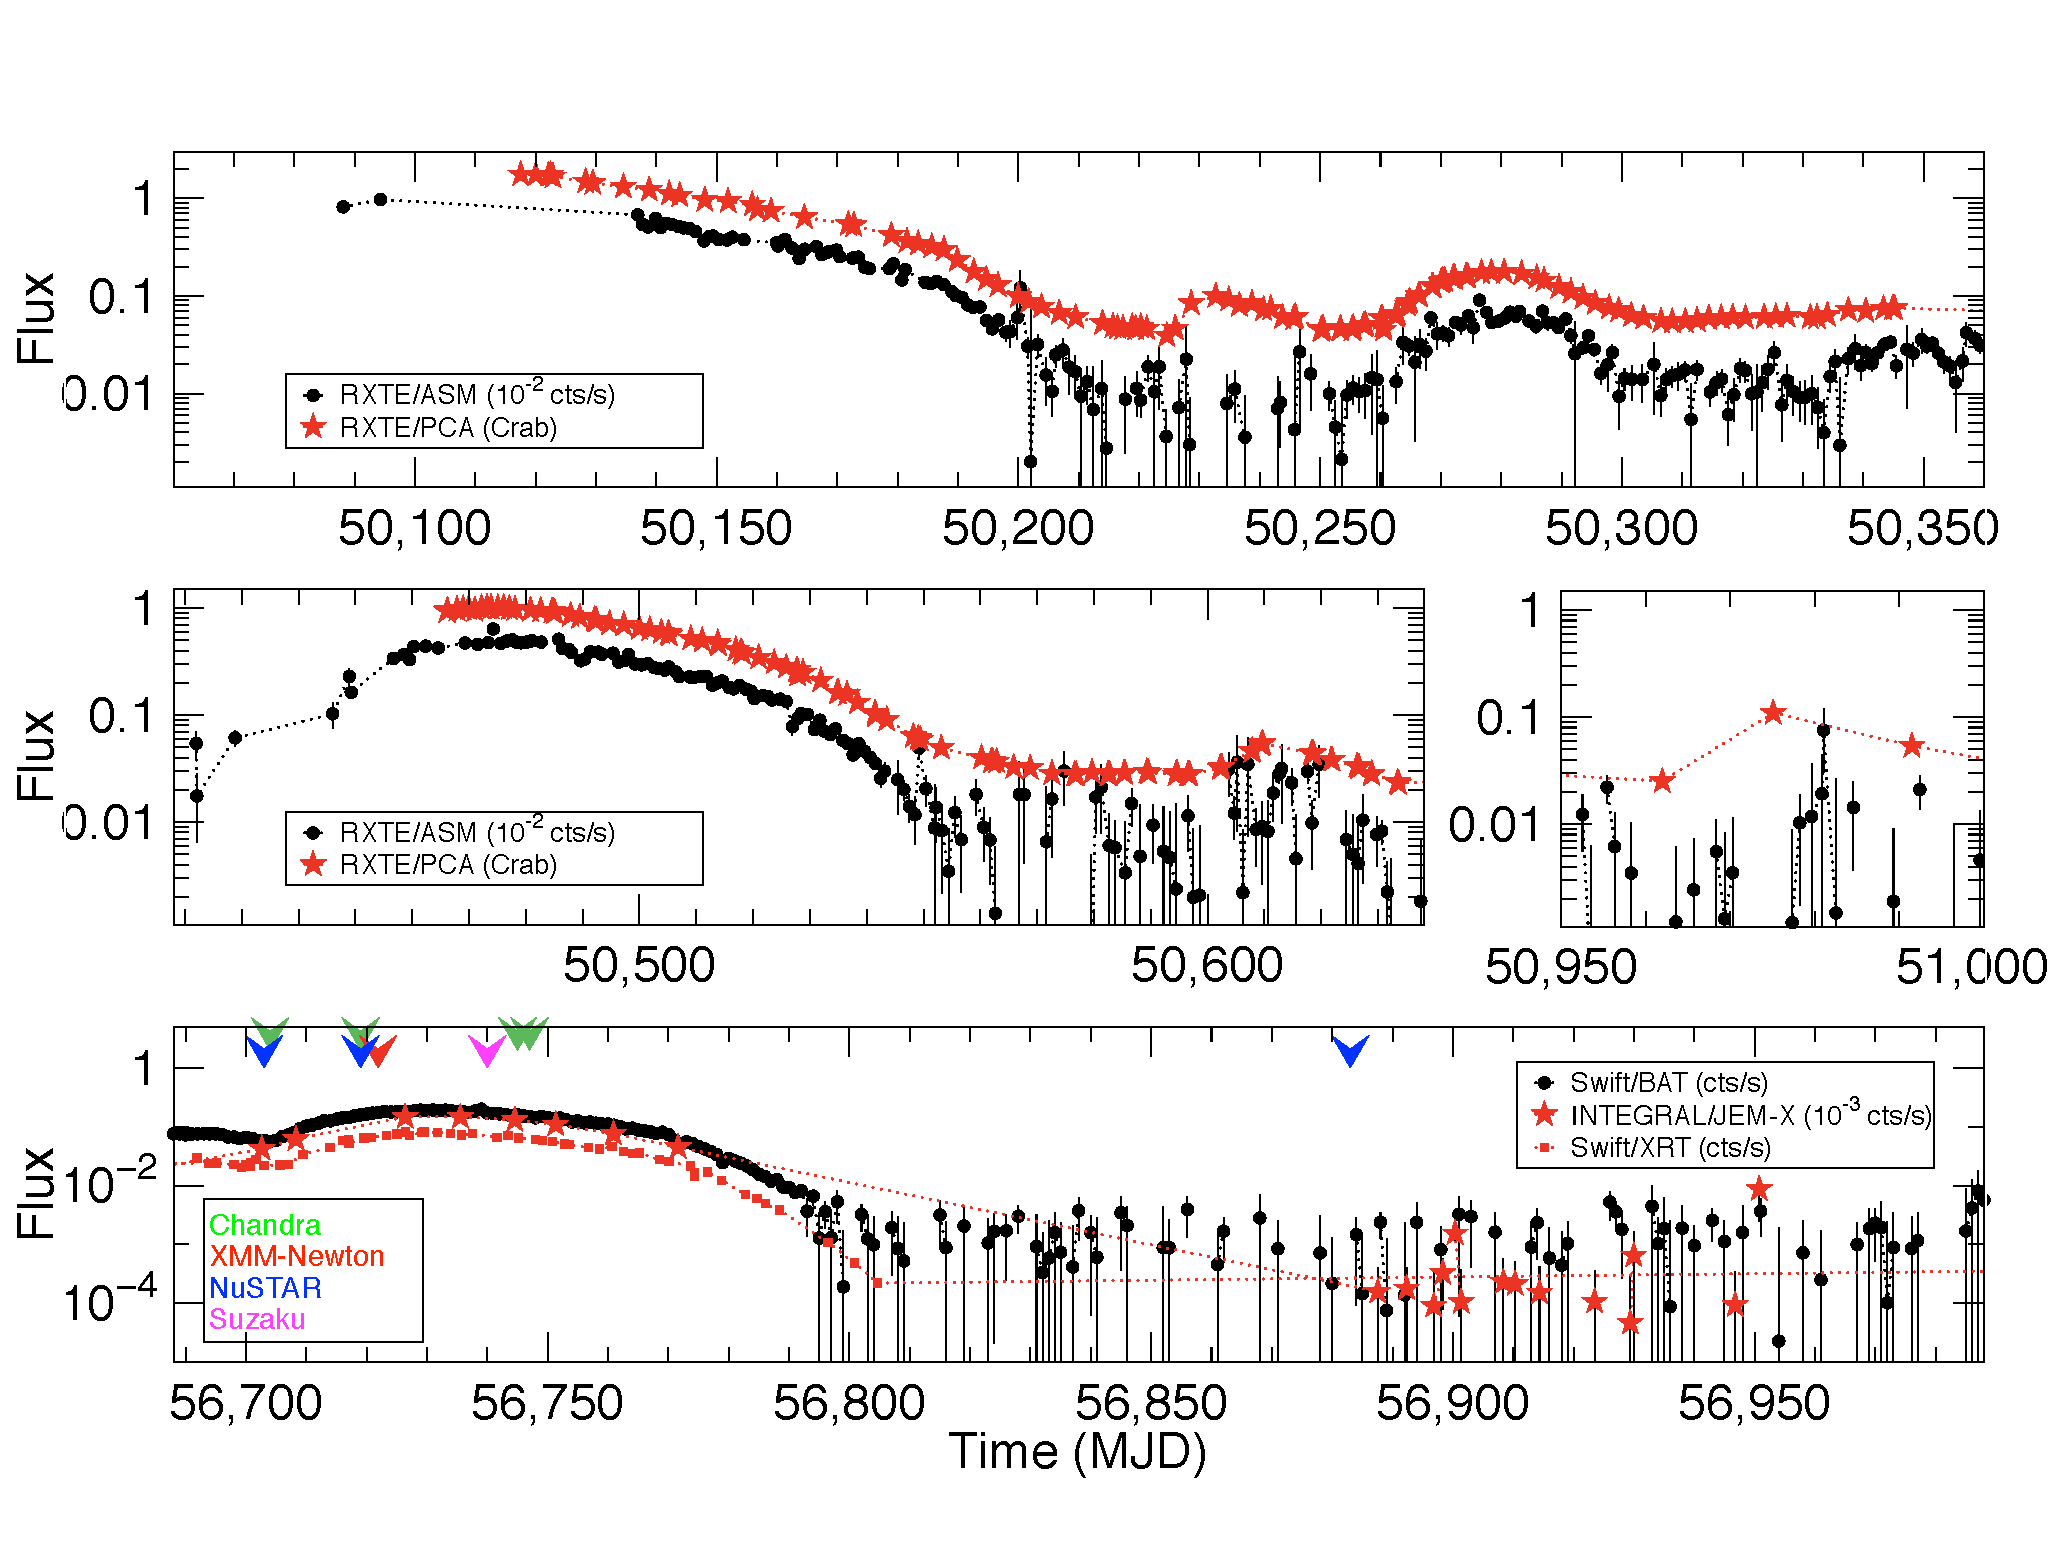
\includegraphics[width=.9\linewidth, trim={0cm 0 0cm 0},clip]{images/lc_comp.pdf}
  \caption[Comparisons of three outbursts of the Bursting Pulsar.]{\small \indexbat\indexxrt\indexrxte\indexasm\indexpca\indexintegral\indexjemx Comparisons of the three outbursts\index{Outburst} of the Bursting Pulsar\index{Bursting Pulsar} reported on in this chapter.  Times corresponding to pointed observations with \indexchandra\textit{Chandra}, \indexnustar\textit{NuSTAR}, \indexsuzaku\textit{Suzaku}, \indexswift\textit{Swift} and \indexxmm\textit{XMM-Newton} are marked.}
  \label{fig:global_ob}
\end{figure}

\par The Bursting Pulsar\index{Bursting Pulsar} was discovered already in outburst\index{Outburst} on December 12 1995 \citep{Fishman_Discovery}; \index{CGRO@\textit{CGRO}!BATSE}\index{CGRO@\textit{CGRO}}\textit{CGRO}/BATSE data suggest that this outburst began several days earlier on December 3 \citep{Paciesas_BPDiscovery,Bildsten_Rev}.  The main outburst ended around May 10 1996 \citep{Woods_PulseBursts}.  I show the global lightcurve\index{Lightcurve} of this outburst in Figure \ref{fig:global_ob}, Panel 1.  As \indexrxte\textit{RXTE} did not observe the object before or during the peak of Outburst, I can only obtain a lower limit of $\sim1.75$\,Crab for the peak 2--16\,keV flux.
\par There are at least two major rebrightening\index{Re-flare}\index{Rebrightening event|see {Re-flare}} events in the tail of Outburst\index{Outburst} 1, which can be seen clearly  in Figure \ref{fig:global_ob} centred at MJDs of $\sim50235$ and $\sim50280$.  During these rebrightening events, the 2--16\,keV flux peaked at $\sim0.10$ and $\sim0.18$\,Crab respectively.

\par Outburst\index{Outburst} 2 began on December 1 1996 and ended around April 7 1997 \citep{Woods_OB2}.  The 2--16\,keV flux peaked at 1.02\,Crab on MJD 50473; I show the global lightcurve\index{Lightcurve} of this outburst in Figure \ref{fig:global_ob}, Panel 2.  Type II-like\index{X-ray burst!Type II} bursts are seen in \indexpca\textit{RXTE}/PCA lightcurves from Outburst 2 between MJDs 50466 and 50544.  One rebrightening\index{Re-flare} event occurred during the tail of Outburst 2, centred at an MJD of $\sim50615$ with a peak 2--16\,keV flux of $\sim54$\,mCrab.  A second possible rebrightening event occurs at MJD 50975, with a peak 2--16\,keV flux of 11\,mCrab, but the cadence of \textit{RXTE}/PCA observations was too low to unambiguously confirm the existence of a re-flare at this time.

\par Outburst 3\index{Outburst} began on January 31, 2014 \citep{Negoro_OB3,Kennea_BPOutburst} and ended around April 23 (e.g. \citealp{Dai_OB3}).  The daily 0.3--10\,keV Swift/XRT rate peaked at 81\,cts\,s$^{-1}$ on MJD 56729, corresponding to 0.4\,Crab.  I show the global lightcurve\index{Lightcurve} of this outburst in Figure \ref{fig:global_ob}, Panel 3.
\par During the main part of Outburst 3, \indexswift\textit{Swift}, \indexxmm\textit{XMM-Newton} and \indexsuzaku\textit{Suzaku} made one pointed observation each, \indexchandra\textit{Chandra} made four observations, and \indexnustar\textit{NuSTAR} made three observations.  The \textit{Chandra} observation on March 3 2014 was made simultaneously with one of the \textit{NuSTAR} observations (see \citealp{Younes_Expo}).  After the main part of the outburst, the source was not well-monitored, although it remained detectable by \indexbat\textit{Swift}/BAT, and it is unclear whether any rebrightening events occured.  A single \textit{NuSTAR} observation was made during the outburst tail on August 14 2014.

\par As can be seen in Figure \ref{fig:global_ob}, the main section of all three outbursts\index{Outburst} follow a common profile, over a timescale of $\sim150$ days.  A notable difference between outbursts 1 \& 2 is the number of rebrightening\index{Re-flare} events; while I find two re-flares associated with Outburst 1, I only find one associated with Outburst 2 unless I assume the event at MJD 50975 is associated with the outburst.  Additionally, Outburst 2 was at least a factor $\sim1.7$ fainter at its peak than Outburst 1 (see also \citealp{Woods_OB2}), while Outburst 3 was a factor of $\gtrsim4$ fainter at peak than Outburst 1.

\subsubsection{Pulsations}

\par \textsf{A.S.} found pulsations in PCA\indexpca\ data throughout the entirety of Outbursts\index{Outburst} 1 \& 2.  This confirms that the Bursting Pulsar\index{Bursting Pulsar} was active as an X-ray pulsar\index{Pulsar} in all of my observations, leading us to conclude that all the types of X-ray burst\index{X-ray burst!Type II} that we see are from the Bursting Pulsar.  In Figure \ref{fig:pulsovertime}, I show that the amplitude of these pulsations approximately followed the intensity of the source in both outbursts, but there were significant deviations from this trend.  These deviations will require further investigation, and a comparison with other accreting\index{Accretion} pulsar systems.  Previous studies have shown that pulsations were also present during Outburst 3 (e.g. \citealp{Sanna_BP}).

\begin{figure}
  \centering
  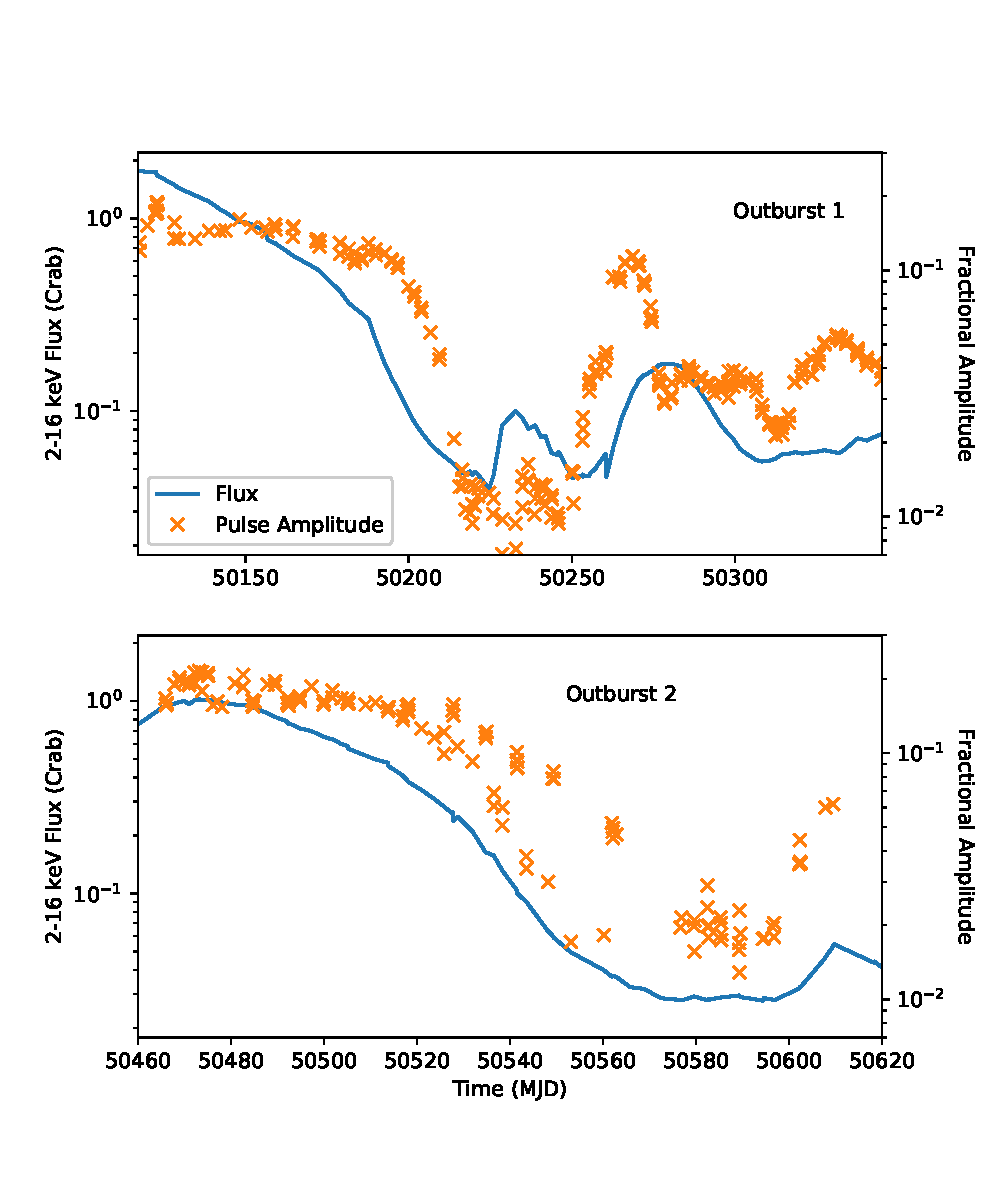
\includegraphics[width=.9\linewidth, trim={0.4cm 1cm 0cm 1cm},clip]{images/PulseAmp.eps}
  \caption[\textit{RXTE}/PCA lightcurves of Outbursts 1 \& 2 of the Bursting Pulsar, overlaid with plots showing how the fractional RMS of the 2.4\,Hz pulsation changes as a function of time.]{\small 2--16\,keV \indexpca\textit{RXTE}/PCA lightcurves\index{Lightcurve} of Outbursts\index{Outburst} 1 \& 2 of the Bursting Pulsar\index{Bursting Pulsar} (solid blue), overlaid with plots showing how the fractional RMS\index{RMS} of the 2.4\,Hz pulsation associated with the pulsar\index{Pulsar} changes as a function of time during these outbursts (orange crosses).}
  \label{fig:pulsovertime}
\end{figure}

\subsubsection{Bursting Behaviour}

\label{sec:bburstevo}

\par Bursts\index{X-ray burst} are seen in \indexpca\textit{RXTE}/PCA lightcurves\index{Lightcurve} from the start of the Outburst\index{Outburst} 1 (e.g. \citealp{Kouveliotou_BP}).  These bursts occur until around MJD 50200, as the source flux falls below $\sim0.1$\,Crab in the 2--16\,keV band.  
\par During the latter part of the first rebrightening\index{Re-flare} after Outburst 1\index{Outburst}, between MJDs 50238 and 50246, \textsf{A.A.} found Type II\index{X-ray burst!Type II}-like bursts\index{X-ray burst} with amplitudes $\sim2$ orders of magnitude smaller than those found during the main outburst event.  These gradually increased in frequency throughout this period of time until evolving into a period of highly structured variability\index{Variability} which persisted until MJD 50261.
\par In Outburst\index{Outburst} 2, Type II\index{X-ray burst!Type II} bursts occured between MJDs $\sim50466$ and $50542$.  Low-amplitude Type II-like bursts\index{X-ray burst} were seen during the latter stages of the main outburst, between MJDs 50562 and 50577.  These again evolved into a period of highly structured variability\index{Variability}; this persisted until MJD 50618, just after the peak of the rebrightening\index{Re-flare} event.
\par High-amplitude Type II\index{X-ray burst!Type II} bursts were also seen in Outburst\index{Outburst} 3 (e.g. \citealp{Linares_NewBurst}).  As no soft ($\lesssim10\,$keV) X-ray instrument was monitoring the Bursting Pulsar\index{Bursting Pulsar} during the latter part of Outburst 3, it is unknown whether this Outburst showed the lower-amplitude bursting behaviour seen at the end of Outbursts 1 \& 2.  Low amplitude bursting behaviour is not seen in the pointed \textit{NuSTAR} observation which was made during this time.

\subsection{Categorizing Bursts}

\label{sec:classes}

\par \textsf{A.A.} and I found that bursts\index{X-ray burst} in the Bursting Pulsar\index{Bursting Pulsar} fall into a number of discrete classes, lightcurves\index{Lightcurve} from which I show in Figure \ref{fig:classes}.  These classes are as follows:

\begin{figure}
  \centering
  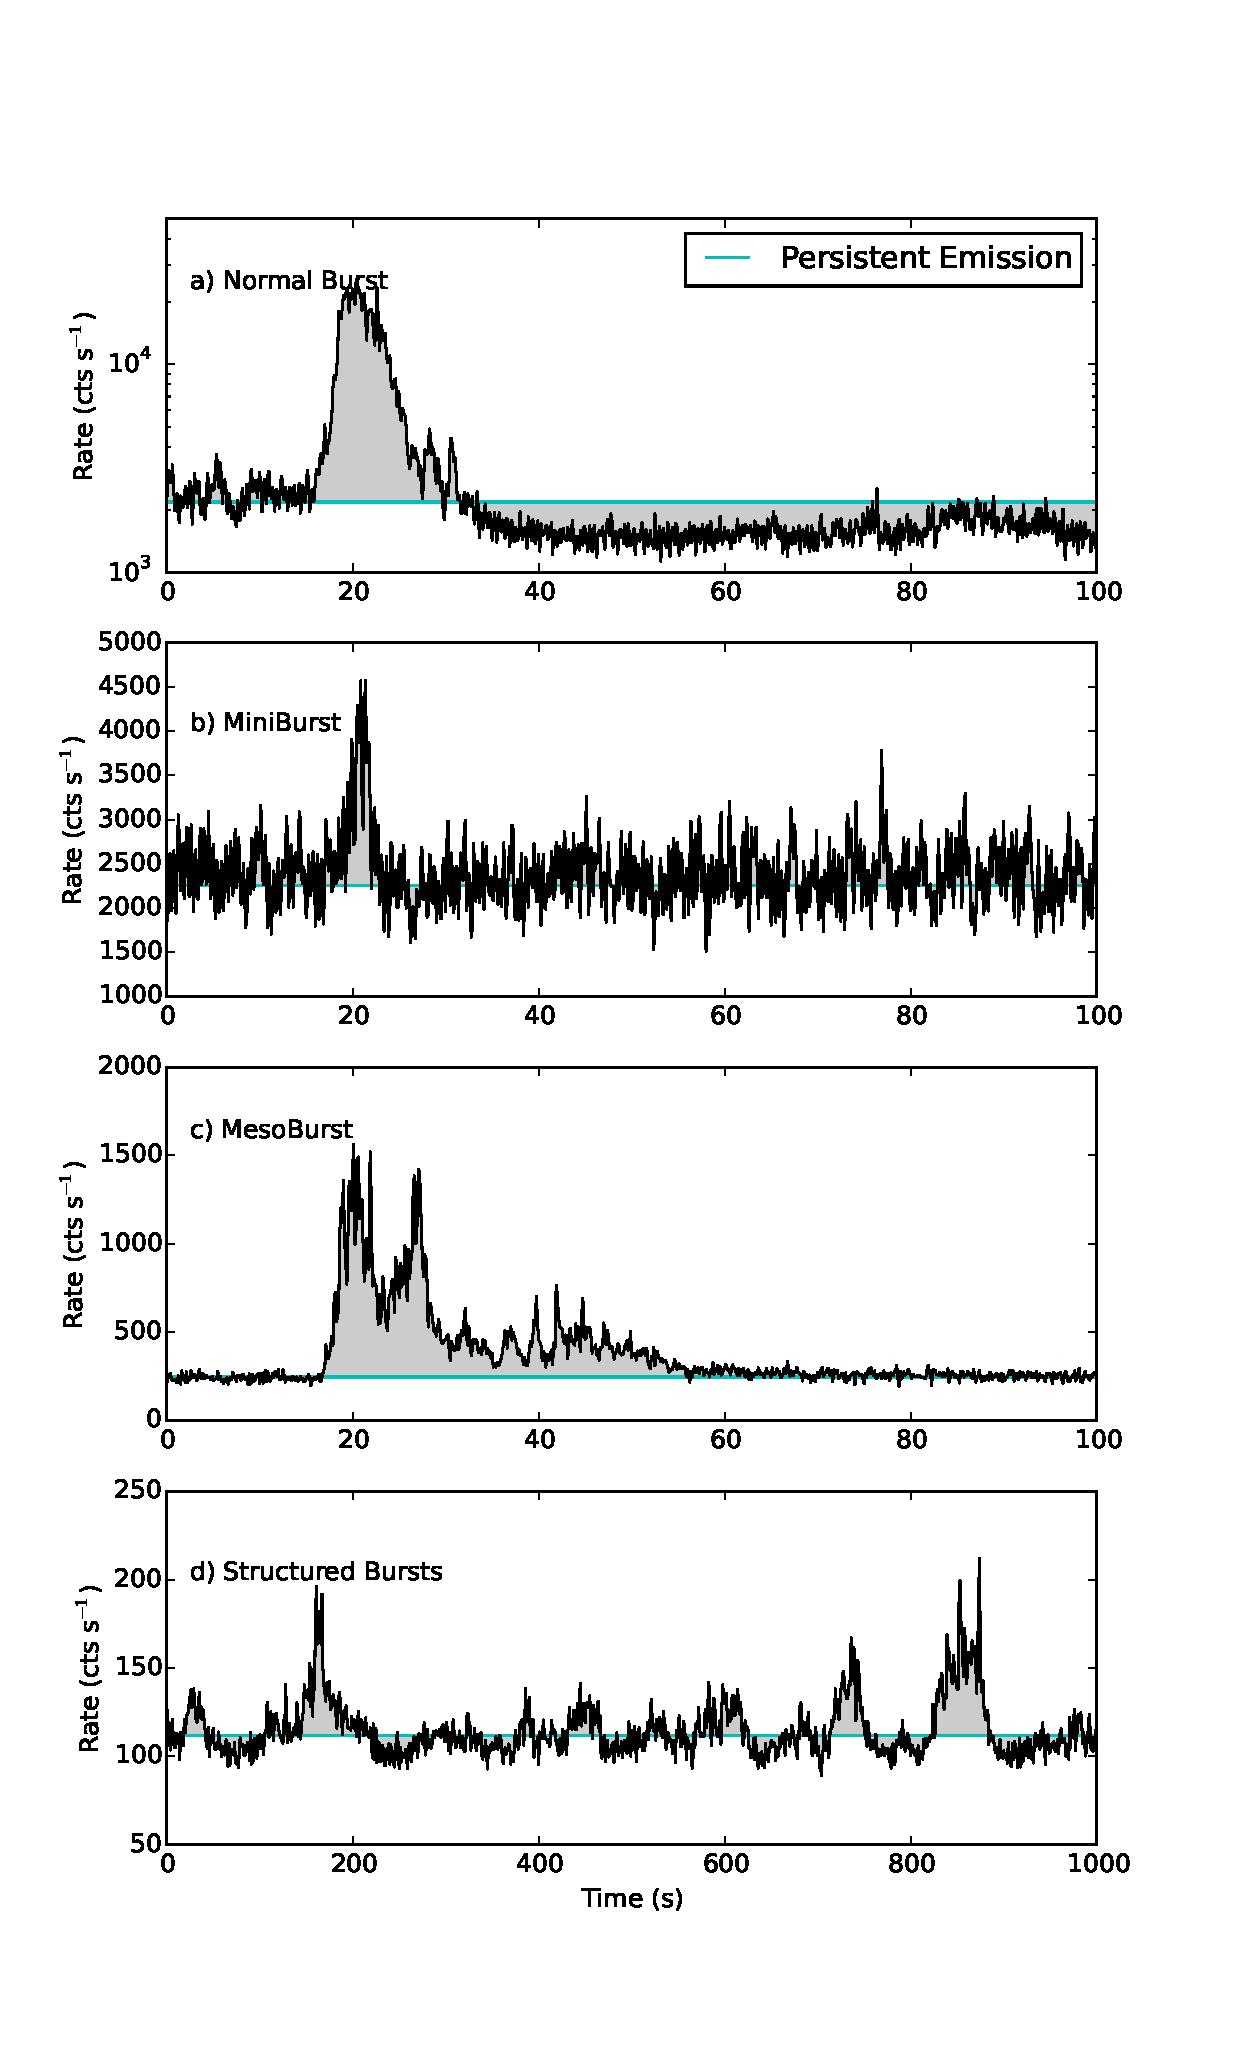
\includegraphics[width=.9\linewidth, trim={0.7cm 2.1cm 1.5cm 3.4cm},clip]{images/comp_bursts.eps}
  \caption[Lightcurves for the four classes of bursting behaviour identified in the Bursting Pulsar.]{\small 2--49\,keV lightcurves\index{Lightcurve} for the four classes of bursting\index{X-ray burst} behaviour identified in this chapter: \textbf{a)} Normal Burst\index{Normal burst}, \textbf{b)} Miniburst\index{Miniburst}, \textbf{c)} Mesoburst\index{Mesoburst}, \textbf{d)} Structured Bursts\index{Structured bursting}.  Note that Panel \textbf{d} is plotted with a different time scaling to the other panels so as to better show the behaviour of Structured Bursting.  On all figures the median count rate, which I use as a proxy for the persistent emission\index{Persistent emission}, is plotted in cyan.  Lightcurves \textbf{a}-\textbf{c} are binned to 0.125\,s, while lightcurve \textbf{d} is binned to 1\,s.}
  \label{fig:classes}
\end{figure}

\begin{itemize}
\item Normal Bursts\index{Normal burst} (Figure \ref{fig:classes}, Panel a): the brightest bursts\index{X-ray burst} seen from this source, with peak count 1\,s binned rates of $\sim10000$\,cts\,s$^{-1}$\,PCU$^{-1}$, and recurrence\index{Recurrence time} timescales of order $\sim1000$\,s.  These bursts are roughly Gaussian\index{Gaussian profile} in shape with durations of $\sim10$\,s, and are followed by a `dip'\index{Dip} in the persistent emission count rate with a duration of order 100\,s (see also e.g. \citealp{Giles_BP}).
\item Minibursts\index{Miniburst} (Figure \ref{fig:classes}, Panel b): faint bursts\index{X-ray burst} with 1\,s-binned peak count rates of $\sim2$ times the persistent emission\index{Persistent emission} count rate.  Minibursts are variable, with duration timescales between $\sim5$--50\,s.  These bursts are also sometimes followed by dips\index{Dip} similar to those seen after Normal Bursts.
\item Mesobursts\index{Mesoburst} (Figure \ref{fig:classes}, Panel c): Type II-like\index{X-ray burst}\index{X-ray burst!Type II} bursts.  These bursts differ from Normal\index{Normal burst} Bursts in that they do not show well-defined subsequent `dips'\index{Dip}.  They are also fainter than Normal Bursts, with peak count 1\,s binned count rates of $\sim1000$\,cts\,s$^{-1}$\,PCU$^{-1}$.  Their burst profiles show fast rises on timescales of seconds, with slower decays and overall durations of $\sim50$\,s.  The structure of the bursts is very non-Gaussian\index{Gaussian profile}, appearing as a small forest of peaks in lightcurves\index{Lightcurve}.
\item Structured Bursts\index{Structured bursting} (Figure \ref{fig:classes}, Panel d): the most complex class of bursting\index{X-ray burst} behaviour we observe from the Bursting Pulsar\index{Bursting Pulsar}, consisting of patterns of flares\index{Flare} and dips\index{Dip} in the X-ray lightcurve\index{Lightcurve}.  The amplitudes of individual flares are similar to those of the faintest Mesobursts\index{Mesoburst}.  The recurrence timescale\index{Recurrence time} is of the order of the timescale of an individual flare, meaning that is it difficult to fully separate individual flares of this class.
\end{itemize}

\par In the upper panel of Figure \ref{fig:jointhist} I show a histogram of persistent-emission\index{Persistent emission}-subtracted peak count rates for all Normal\index{Normal burst} and Mesobursts\index{Mesoburst} observed by \indexrxte\textit{RXTE}.  I split these two classes based on the bimodal distribution in peak count rate as well as the lack of dips\index{Dip} in Mesobursts.  In the lower panel of Figure \ref{fig:jointhist}, I show the histogram of peak count rates for all Normal\index{Normal burst} and Minibursts\index{Miniburst} observed by \indexrxte\textit{RXTE} as a fraction of the persistent emission at that time.  I split these two classes based on the strongly bimodal distribution in fractional amplitude.

\begin{figure}
  \centering
  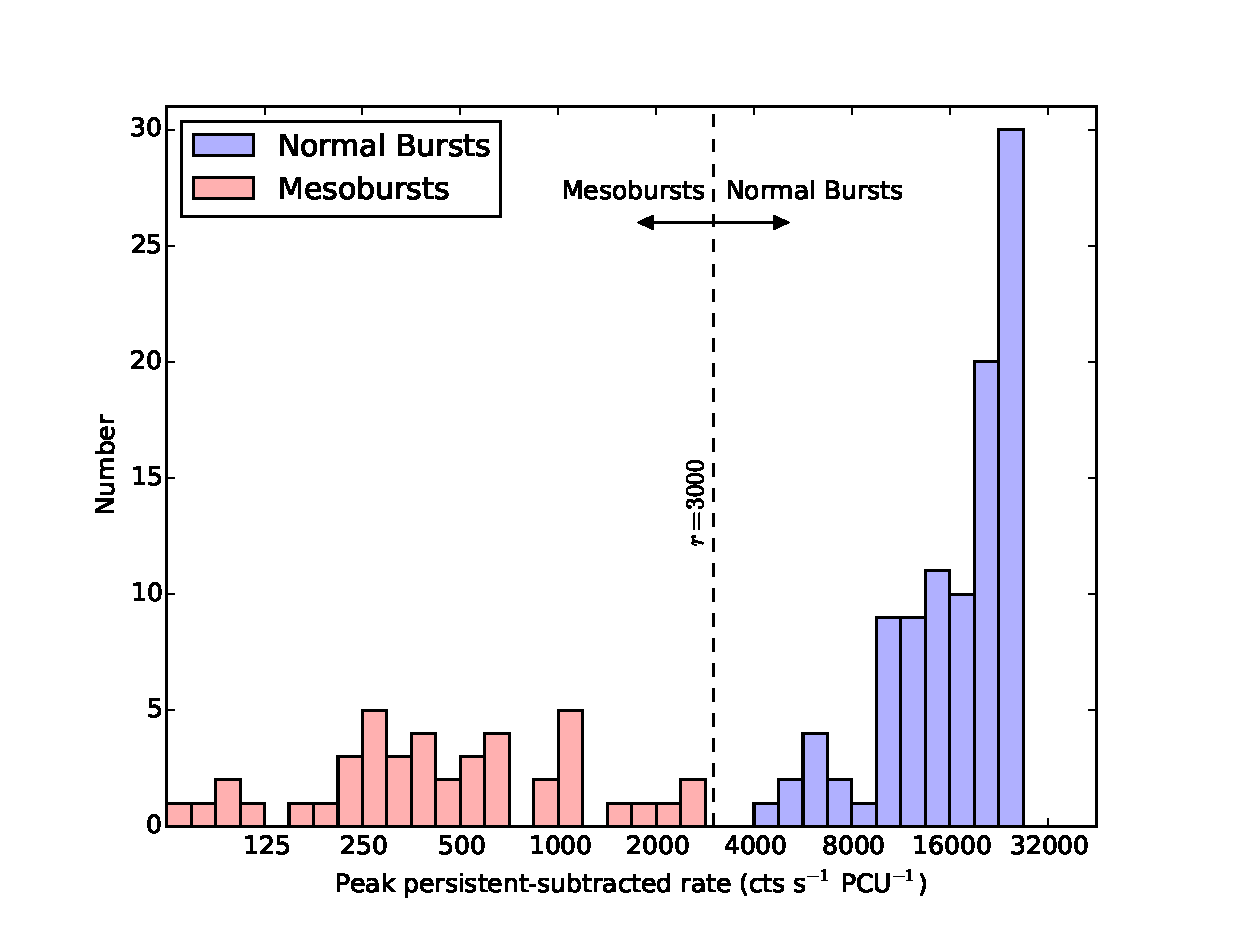
\includegraphics[width=.8\linewidth, trim={1.3cm 0.4cm 2.0cm 0.8cm},clip]{images/norm_meso_sep.eps}
  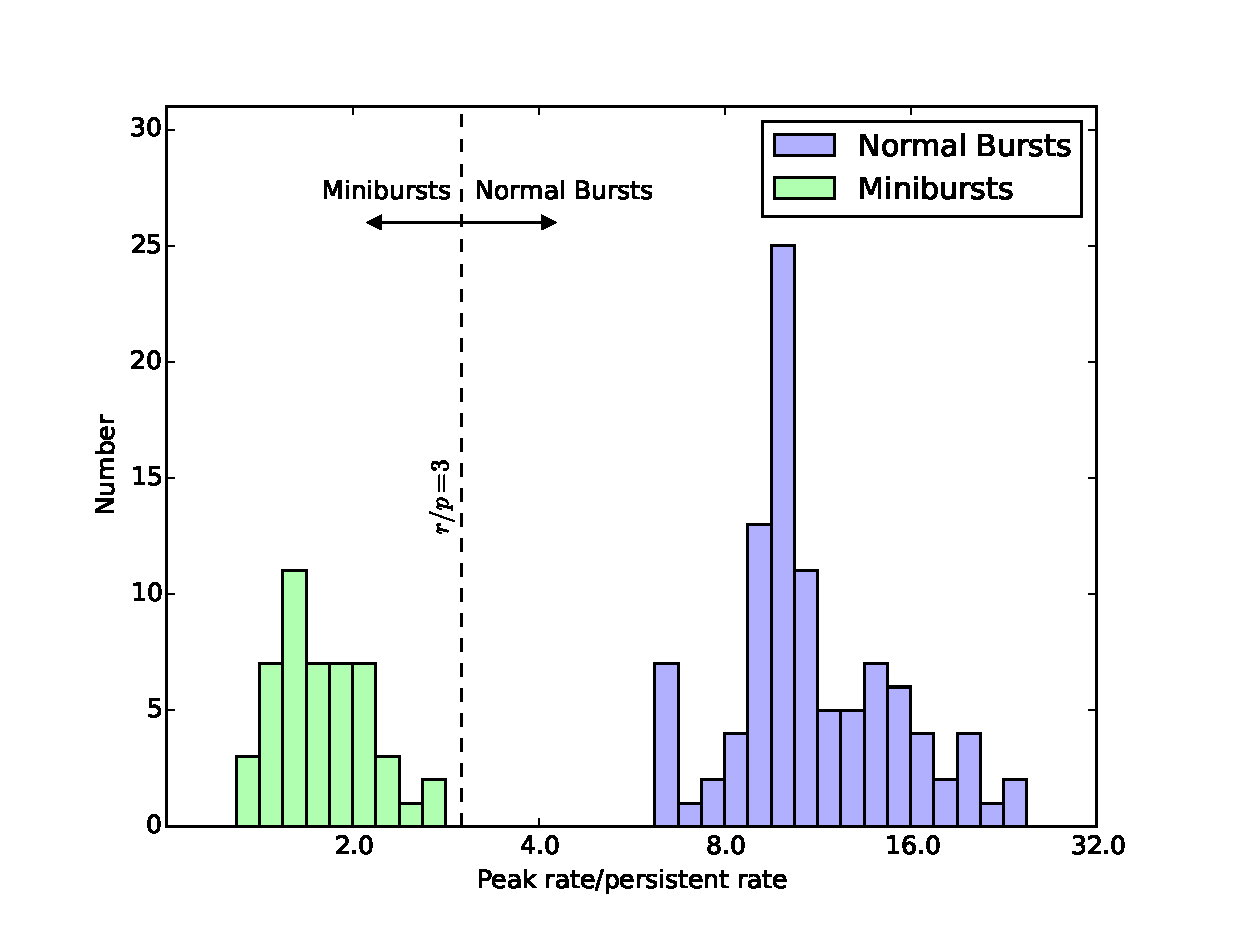
\includegraphics[width=.8\linewidth, trim={1.3cm 0.4cm 2.0cm 0.8cm},clip]{images/norm_mini_sep.eps}
  \caption[Histogram of the peak 1\,s binned peak count rates during Normal Bursts, Mesobursts and Minibursts as seen by \textit{RXTE}]{\small \textbf{Upper Panel:} A histogram of the peak 1\,s binned peak count rates of the joint population\index{Population study} of all Normal\index{Normal burst} and Mesobursts\index{Mesoburst} seen by \indexrxte\textit{RXTE}.  The dashed line indicates the position of the threshold above which I consider a Type II\index{X-ray burst!Type II}-like burst\index{X-ray burst} to be a Normal Burst.  The resultant split of the population into Normal and Mesobursts is indicated by blue and red shading respectively.  The skewed shape of the distribution of Normal Bursts is due to the effects of dead-time\index{Dead-time} putting an effective cap on their maximum observed intensity.
 \textbf{Lower Panel:} A histogram of the peak 1\,s binned peak count rates of the joint population of all Normal and Minibursts\index{Miniburst} seen by \textit{RXTE}, divided by the persistent emission count rate at that time.  The dashed line indicates the position of the threshold below which I consider a burst to be a Miniburst.  The resultant split of the population into Normal and Minibursts is indicated by blue and green shading respectively.
  Note that the $x$-axis of both plots is logarithmic, and so number density is not preserved.}
  \label{fig:jointhist}
\end{figure}

\par I also find 6 bursts\index{X-ray burst} with fast ($\sim1$\,s) rises and exponential decays that occur during the lowest flux regions of the outburst\index{Outburst} ($\lesssim50$\,mCrab).  \citet{Strohmayer_BPFieldTypeI} and \citet{Galloway_TypeI} have previously identified these bursts as being Type I X-ray\index{X-ray burst!Type I} bursts from another source in the \indexrxte\textit{RXTE} field of view.  To show that these unrelated Type I bursts would not be confused with Minibursts\index{Miniburst}, I add examples of the Type I bursts to lightcurves from observations containing Minibursts.  I find that the peak count rates in Type I bursts are roughly equal to the amplitude of the noise in the persistent\index{Persistent emission} flux in these observations, hence they would not be detected by my algorithms.
\par I show when in Outbursts\index{Outburst} 1 \& 2 each type of burst was observed in Figures \ref{fig:ob_evo1} and \ref{fig:ob_evo2} respectively.  Normal Bursts\index{Normal burst} and Minibursts\index{Miniburst} (red) occur during the same periods of time from around the peak of an outburst until the persistent emission\index{Persistent emission} falls beneath $\sim0.1$\,Crab; assuming an Eddington Limit\index{Eddington limit} of $\sim1$\,Crab (e.g \citealp{Sazonov_BPGranat}), this corresponds to an Eddington ratio of $\sim0.1$.  After this point, bursting\index{X-ray burst} is not observed for a few tens of days.  Mesobursts\index{Mesoburst} (blue) begin at the end of a rebrightening\index{Re-flare} event in Outburst 1 and during the final days of the main part of the outburst in Outburst 2.  Structured Bursts\index{Structured bursting} (yellow) occur during the first part of a rebrightening event in both outbursts.  Although there was a second rebrightening event after Outburst 1, neither Mesobursts nor Structured Bursts were observed at this time.  Based on this separation, as well as differences in structure, I treat each class of burst separately below.

\begin{figure}
  \centering
  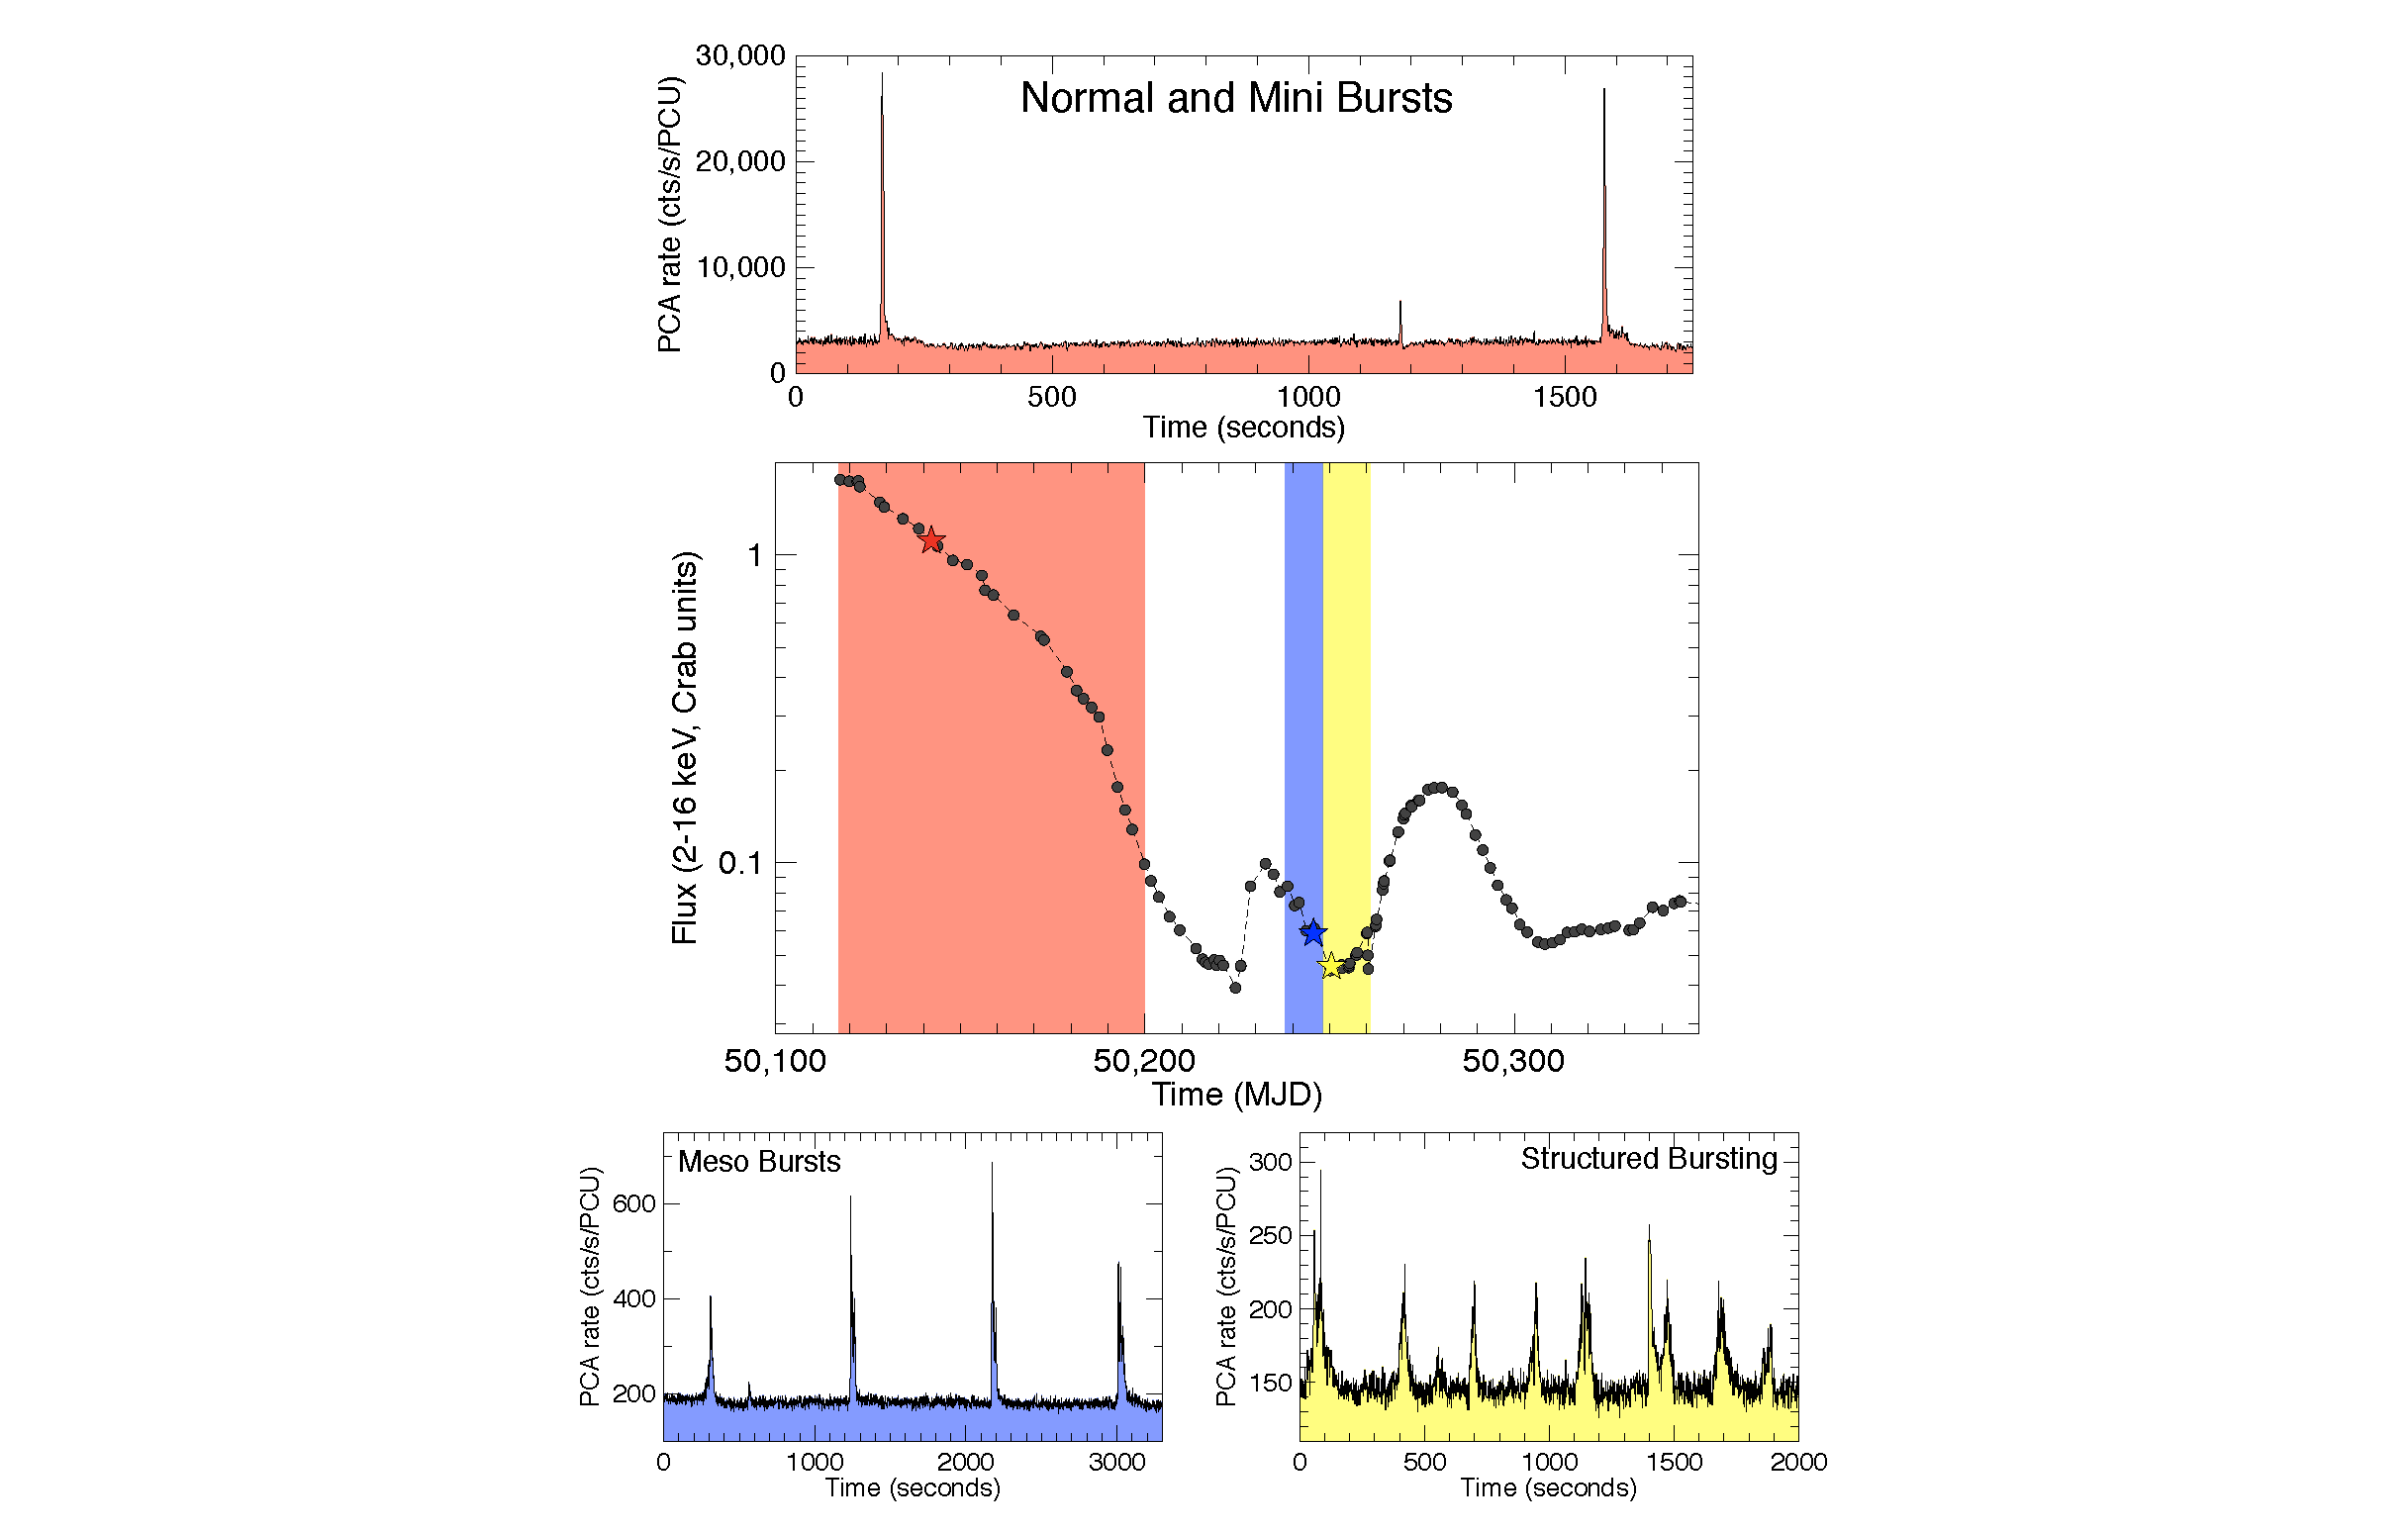
\includegraphics[width=.9\linewidth, trim={9.5cm 0cm 10cm 0cm},clip]{images/obevo1.pdf}
  \caption[Lightcurve of the 1995--1996 outburst of the Bursting Pulsar, highlighting periods of time during which Mesobursts, Structured Bursts or Normal and Mini bursts are observed.]{\small Central panel shows the global 2--16\,keV \indexpca\textit{RXTE}/PCA lightcurve\index{Lightcurve} of the 1995--1996 outburst\index{Outburst} of the Bursting Pulsar\index{Bursting Pulsar}, highlighting periods of time during which Mesobursts\index{Mesoburst} (blue) Structured Bursts\index{Structured bursting} (yellow) or Normal\index{Normal burst} and Mini\index{Miniburst} bursts (red) are observed.  A single Mesoburst was also observed on MJD 50253, during the period of the outburst highlighted in yellow (see Figure \ref{fig:meso_in_struc}).  Other panels show example lightcurves which contain the aforementioned types of bursting\index{X-ray burst} behaviour.  See section \ref{sec:classes} for a detailed treatment of burst classification.  Fluxes reported in units of Crab.}
  \label{fig:ob_evo1}
\end{figure}

\begin{figure}
  \centering
  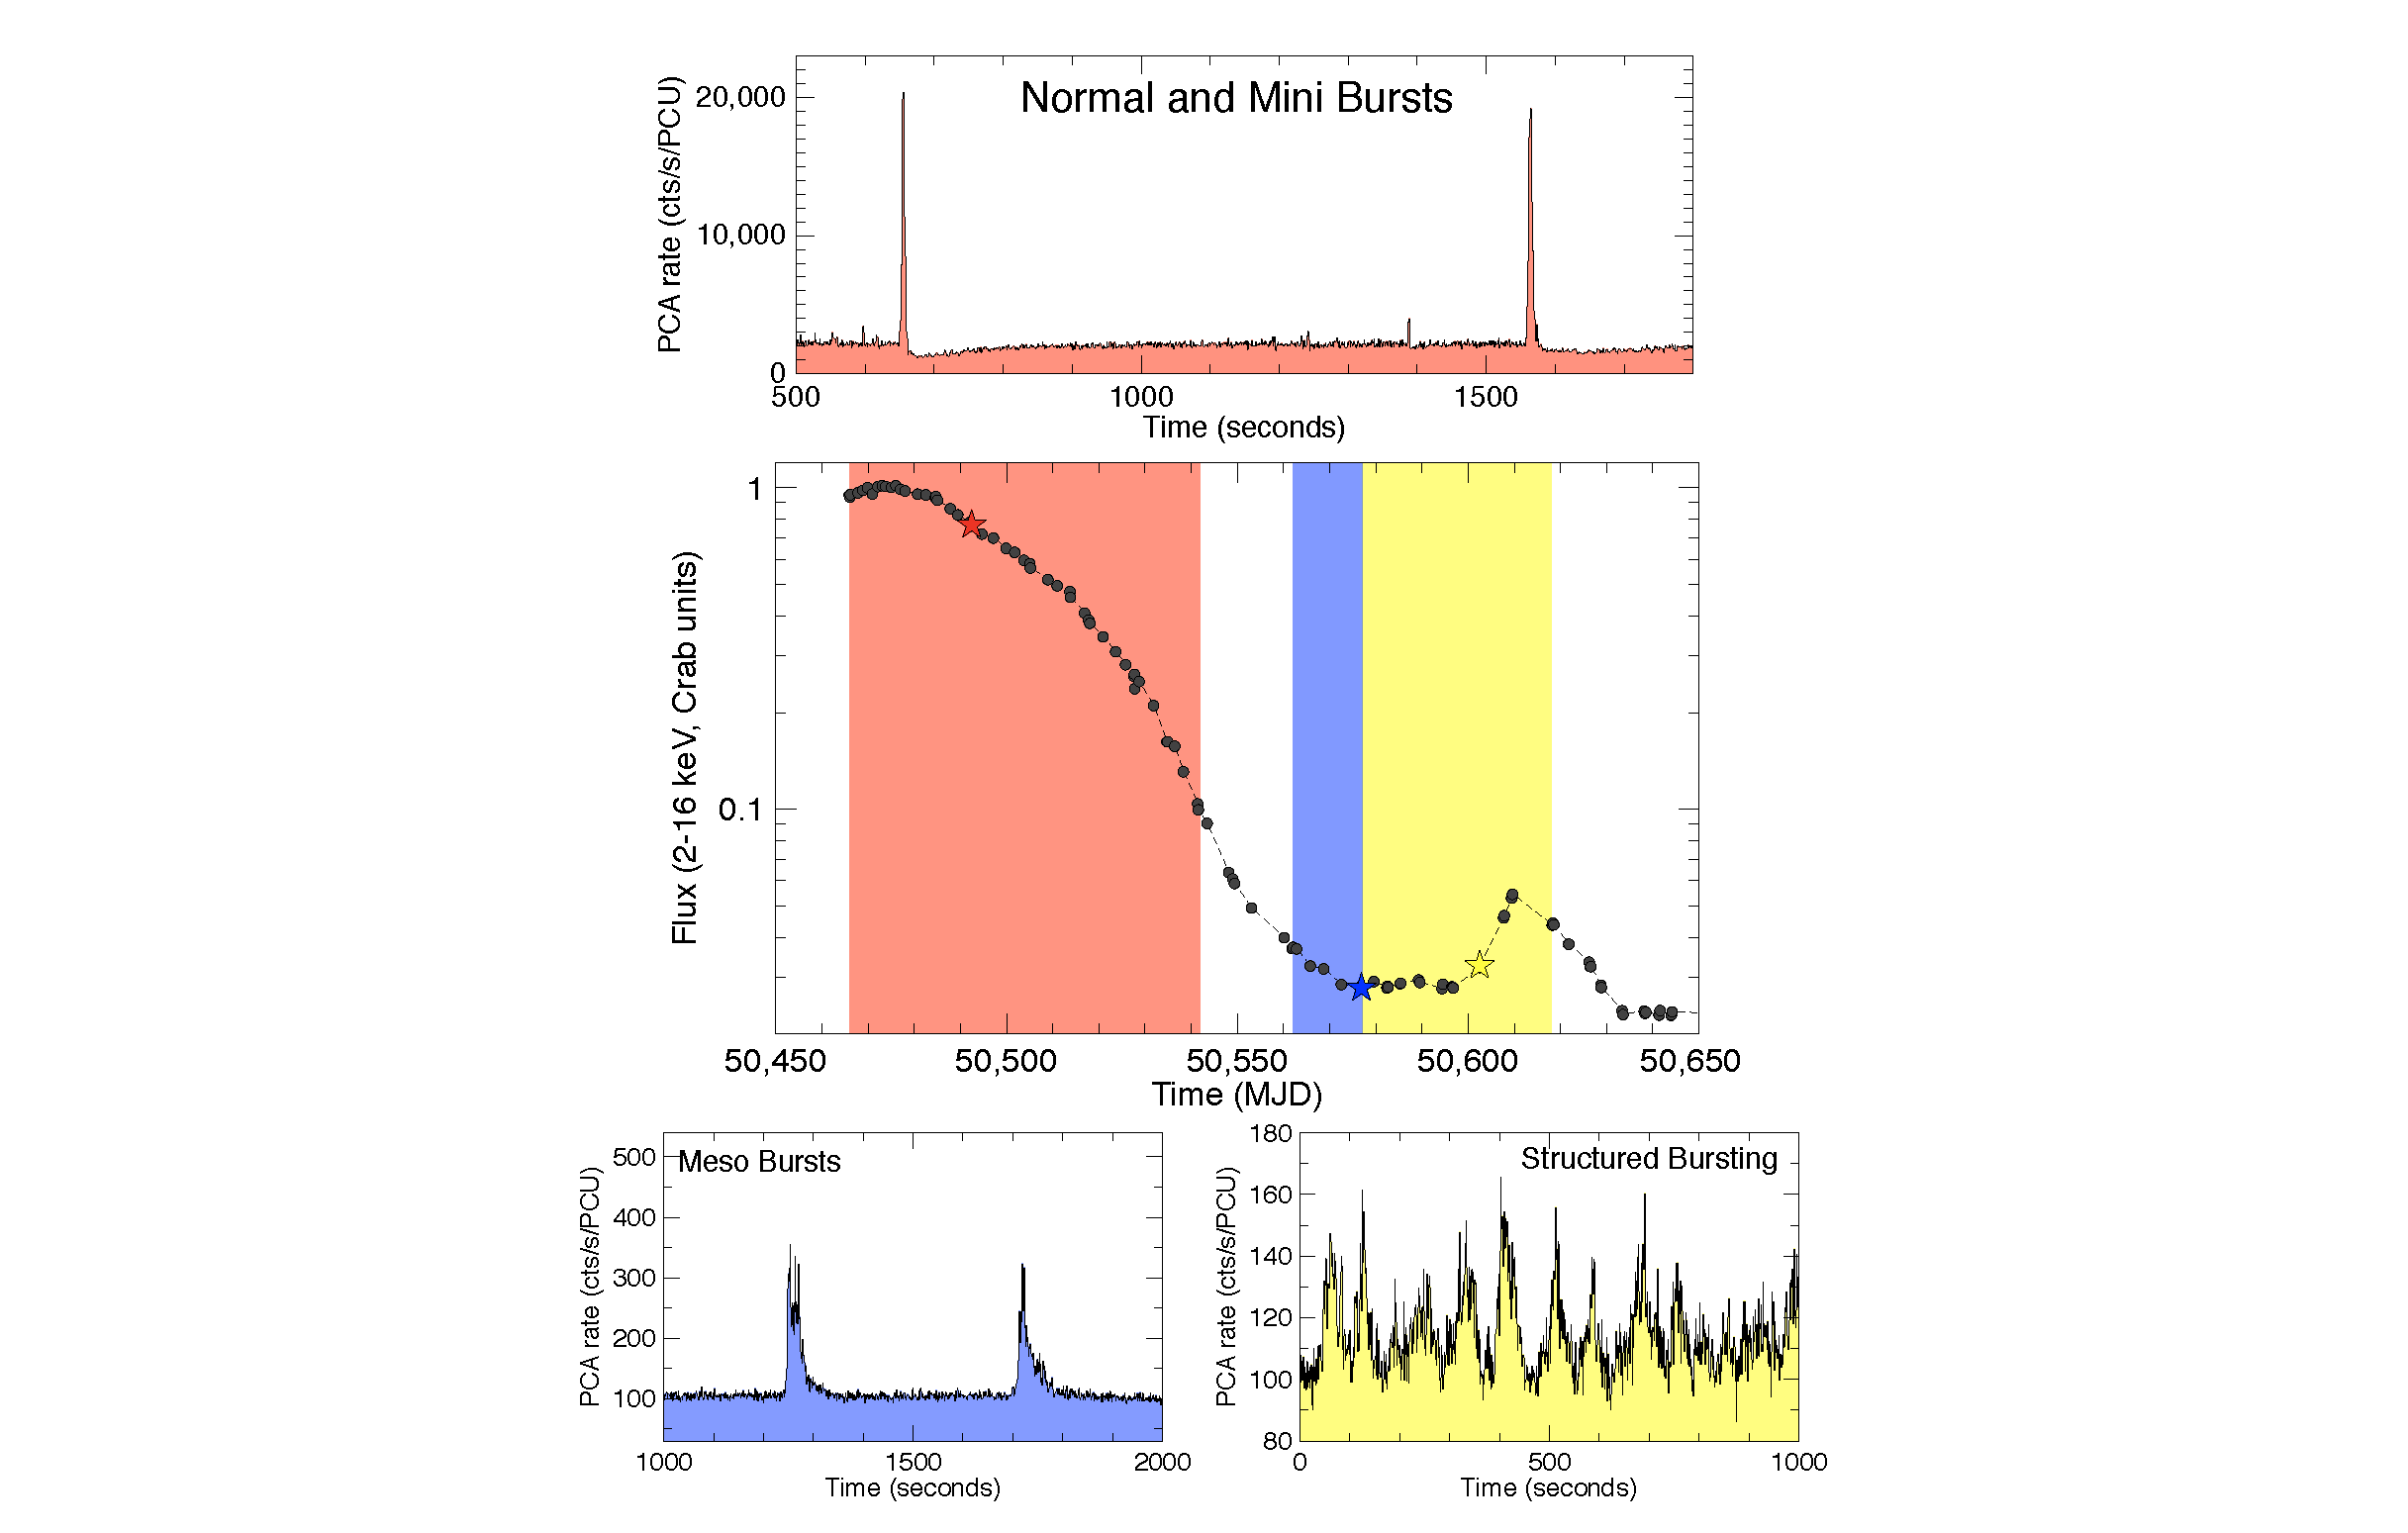
\includegraphics[width=.9\linewidth, trim={9.5cm 0cm 10cm 0cm},clip]{images/obevo2.pdf}
  \caption[Lightcurve of the 1997--1999 outburst of the Bursting Pulsar, highlighting periods of time during which Mesobursts, Structured Bursts or Normal and Mini bursts are observed.]{\small Central panel shows the global 2--16\,keV \indexpca\textit{RXTE}/PCA lightcurve\index{Lightcurve} of the 1997--1999 outburst\index{Outburst} of the Bursting Pulsar\index{Bursting Pulsar}, highlighting periods of time during which Mesobursts\index{Mesoburst} (blue) Structured Bursts\index{Structured bursting} (yellow) or Normal\index{Normal burst} and Mini\index{Miniburst} bursts (red) are observed.  Other panels show example lightcurves which contain the aforementioned types of bursting behaviour\index{X-ray burst}.}
  \label{fig:ob_evo2}
\end{figure}

\subsection{Normal Bursts}

\label{sec:Normal_Bursts}

\par I define Normal Bursts\index{Normal burst} as the set of all bursts\index{X-ray burst} with a persistent-emission\index{Persistent emission}-subtracted peak 1\,s binned \indexpca\textit{RXTE}/PCA-equivalent count rate above 3000\,cts\,s$^{-1}$\,PCU$^{-1}$.  Normal Bursts account for 99 out of the 190\footnote{This number does not include Structured Bursts\index{Structured bursting} as their complex structure makes them difficult to separate.} bursts identified for this study.  They are observed during all three outbursts\index{Outburst} covered in this study.  They occurred between MJDs 50117 and 50200 in Outburst 1, and between 50466 and 50542 in Outburst 2; during these intervals, \indexrxte\textit{RXTE} observed the source for a total of 192\,ks.  See Table \ref{tab:staretimes} to compare these with numbers for the other classes of burst identified in this study.  Normal Bursts occur during the same time intervals in which Minibursts\index{Miniburst} are present.  In both of these outbursts, the period of Normal and Minibursts correspond to the time between the peak of the outburst and and the time that the persistent intensity falls below $\sim0.1$\,Crab.

\begin{table}
\centering
\begin{tabular}{llll}
\hline
\hline
\scriptsize  Bursting Mode &\scriptsize Bursts &\scriptsize Total Exposure (ks) &\scriptsize Duration (d) \\
\hline
Normal Bursts\index{Normal burst} & 99  & 192 & 76\\
Minibursts\index{Miniburst} & 48 & 192  & 76\\
Mesobursts\index{Mesoburst} & 43 &44 &25\\
Structured Bursts\index{Structured bursting} & - &80 &54 \\
\hline
\hline
\end{tabular}
\caption[Statistics on the population of bursts in the 1996 and 1997 outbursts of the Bursting Pulsar.]{Statistics on the population\index{Population study} of bursts\index{X-ray burst} I use for this study, as well as the duration and integrated \indexpca\textit{RXTE}/PCA exposure time of each mode of bursting.  All numbers are the sum of values for Outbursts\index{Outburst} 1 and 2.  As Normal\index{Normal burst} and Minibursts\index{Miniburst} happen during the same period of time in each outburst, the exposure time and mode duration for these classes of bursting are equal.}
\label{tab:staretimes}
\end{table}

\subsubsection{Recurrence Time}

\par Using Outburst\index{Outburst} 3 data from \indexchandra\textit{Chandra}, \indexxmm\textit{XMM-Newton}, \indexnustar\textit{NuSTAR} and \indexsuzaku\textit{Suzaku}, I find minimum and maximum Normal Burst\index{Normal burst} recurrence times\index{Recurrence time} of $\sim345$ and $\sim5660$\,s respectively\footnote{To avoid double-counting peak pairs, I do not use \textit{NuSTAR} observation 80002017004, which was taken simultaneously with \textit{Chandra} observation 16596.}.  I show the histogram of recurrence times from Outburst 3 in Figure \ref{fig:sep}, showing which parts of the distribution were observed with which observatory.  Compared to data from \textit{Chandra} and \textit{XMM-Newton}, data from \textit{Suzaku} generally suggests shorter recurrence times.  This is likely due to \textit{Suzaku} observations consisting of a number of $\sim2$\,ks windows; as this number is of the same order of magnitude as the recurrence time between bursts, there is a strong selection effect against high recurrence times in the \textit{Suzaku} dataset.
\par From the \indexrxte\textit{RXTE} data I find minimum and maximum Normal Burst\index{Normal burst} recurrence times\index{Recurrence time} of $\sim250$ and $\sim2510$\,s during Outburst\index{Outburst} 1, and minimum and maximum recurrence times of $\sim250$ and $\sim2340$\,s during Outburst 2.  As the length of an \textit{RXTE} pointing ($\lesssim3$\,ks) is also of the same order of magnitude as the recurrence time between bursts, selection effects bias us against sampling pairs of bursts with longer recurrence times, and hence this upper value is likely an underestimate.

\begin{figure}
  \centering
  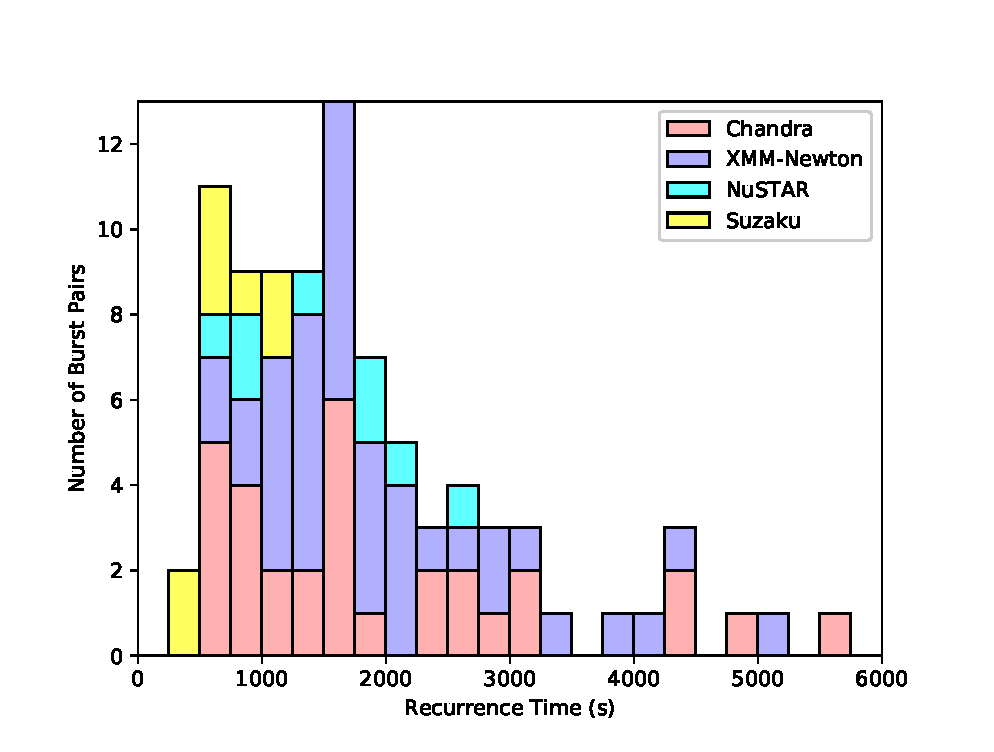
\includegraphics[width=.9\linewidth, trim={0.4cm 0 1.1cm 0},clip]{images/manyinst_stdist.eps}
  \caption[The distribution of recurrence times between consecutive Normal Bursts in Outburst 3.]{\small The distribution of recurrence times\index{Recurrence time} between consecutive Normal Bursts\index{Normal burst} seen in pointed \indexchandra\textit{Chandra}, \indexxmm\textit{XMM-Newton}, \indexnustar\textit{NuSTAR} and \indexsuzaku\textit{Suzaku} observations of Outburst\index{Outburst} 3 of the Bursting Pulsar\index{Bursting Pulsar}.  Distributions of bursts observed by different instruments are stacked on top of each other and colour coded.}
  \label{fig:sep}
\end{figure}

\par To test whether consecutive Normal Bursts\index{Normal burst} are independent events, I tested the hypothesis that bursts are randomly distributed in time in a Poisson distribution\index{Poisson distribution} \citep{Poisson_Distribution}.  Assuming my hypothesis, as well as assuming that the frequency of Normal Bursts does not change during an outburst\index{Outburst} (e.g. \citealp{Aptekar_Recur}), I could concatenate different observations and the resultant distribution of burst times should still be Poissonian.  For each of Outbursts 1 \& 2, I concatenated all \indexrxte\textit{RXTE} data during the Normal Bursting part of the outburst into a single lightcurve\index{Lightcurve}.  I split this concatenated lightcurve into windows of length $w$ and counted how many bursts were in each, forming a histogram of number of bursts per window for the combined set of all bursts.  I fit this histogram with a Poisson probability density function, obtaining the value $\lambda$ which is the mean number of bursts in a time $w$.  $\lambda/w$ is therefore an expression of the true burst frequency per unit time, and should be independent of my choice of $w$.  I tried values of $w$ between 100 and 10000\,s for both outbursts, and found that in all cases $\lambda/w$ depends strongly on $w$.  Therefore my assumptions cannot both be valid, and I rejected the hypothesis that these bursts are from a Poisson distribution with constant $\lambda$.  This in turn suggests at least one of the following must be correct:
\begin{enumerate}
\item The average recurrence time\index{Recurrence time} of bursts was not constant throughout the outburst.  Or:
\item The arrival time of a given burst depends on the arrival time of the preceding burst, and therefore bursts are not independent events.
\end{enumerate}

\subsubsection{Burst Structure}

\label{sec:struc}

\par In the top panel of Figure \ref{fig:norm_overlay} I show a plot of all Normal Bursts\index{Normal burst} observed with \indexrxte\textit{RXTE} overlayed on top of one another.  I find that all Normal Bursts follow a similar burst profile with similar rise and decay timescales but varying peak intensities.  In the lower panel of Figure \ref{fig:norm_overlay} I show a plot of Normal Bursts overlaid on top of each other after being normalised by the persistent emission\index{Persistent emission} count rate in their respective observation.  The bursts are even closer to following a single profile in this figure, suggesting a correlation between persistent emission level in an outburst and the individual fluence of its bursts.

\begin{figure}
  \centering
  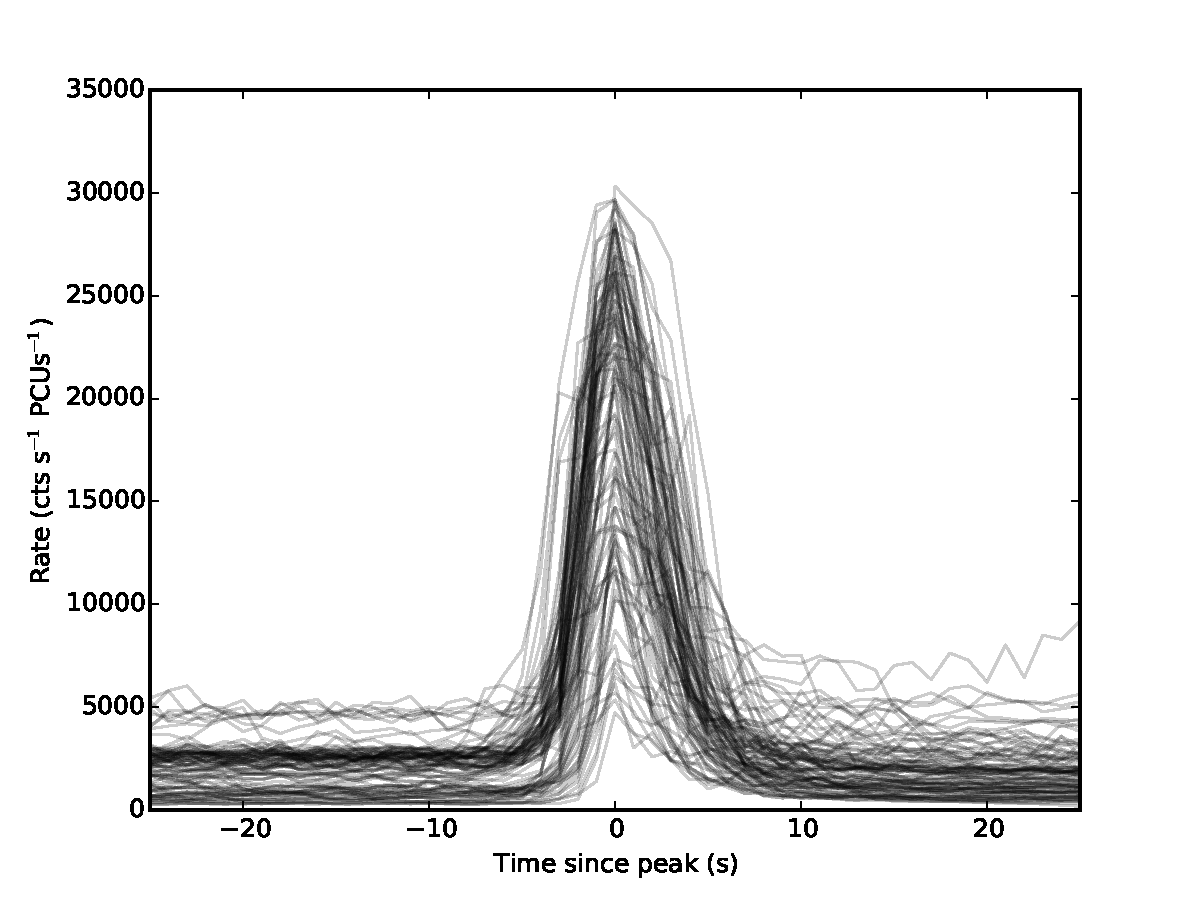
\includegraphics[width=.9\linewidth, trim={0.4cm 0 1.1cm 0},clip]{images/1000norm.pdf}
  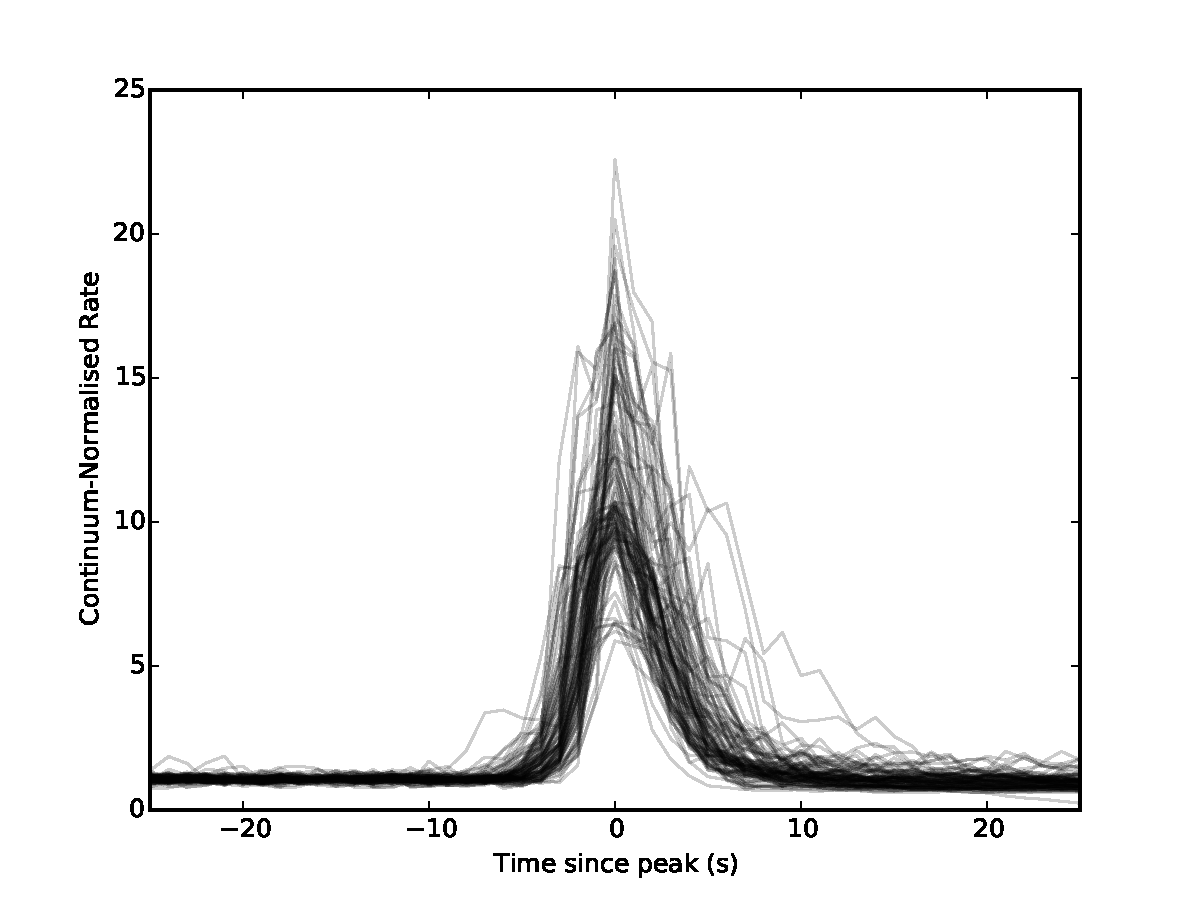
\includegraphics[width=.9\linewidth, trim={0.4cm 0 1.1cm 0},clip]{images/1000norm_renormed.pdf}
  \caption[A plot of every Normal Burst, centred by the time of its peak, overlaid on top of each other to show the existence of a common pulse profile.]{\small \textbf{Top:} a lightcurve\index{Lightcurve} of every Normal Burst\index{Normal burst}, centred by the time of its peak, overlaid on top of each other to show the existence of a common pulse profile.  \textbf{Bottom:} a lightcurve of every Normal Burst in which count rates have been normalised by the persistent emission\index{Persistent emission} count rate during the observation from which each burst was observed.  As the bursts are on average closer to the average pulse profile in this metric, this suggests that the intensity of a burst is roughly dependent on the persistent emission rate.  Some persistent emission-normalised count rates may be artificially low due to dead-time\index{Dead-time} effects.}
  \label{fig:norm_overlay}
\end{figure}

\par The structure of the lightcurve\index{Lightcurve} of a Normal Burst\index{Normal burst} can be described in three well-defined parts:

\begin{enumerate}
\item The main burst: roughly approximated by a skewed Gaussian\index{Gaussian profile} (see e.g. \citealp{Azzalini_Dist}).
\item A `plateau'\index{Plateau}: a period of time after the main burst during which count rate remains relatively stable at a level above the pre-burst rate.
\item A `dip'\index{Dip}: a period during which the count rate falls below the persistent level, before exponentially decaying back up towards the pre-burst level (e.g. \citealp{Younes_Expo}).
\end{enumerate}

\par The dip\index{Dip} is present after every Normal Burst\index{Normal burst} in my \indexrxte\textit{RXTE} sample from Outbursts\index{Outburst} 1 \& 2, whereas the plateau\index{Plateau} is only seen in 39 out of 99.  I show example lightcurves\index{Lightcurve} of bursts with and without plateaus in Figure \ref{fig:w_wo}, which also show that the dip is present in both cases.

\begin{figure}
  \centering
  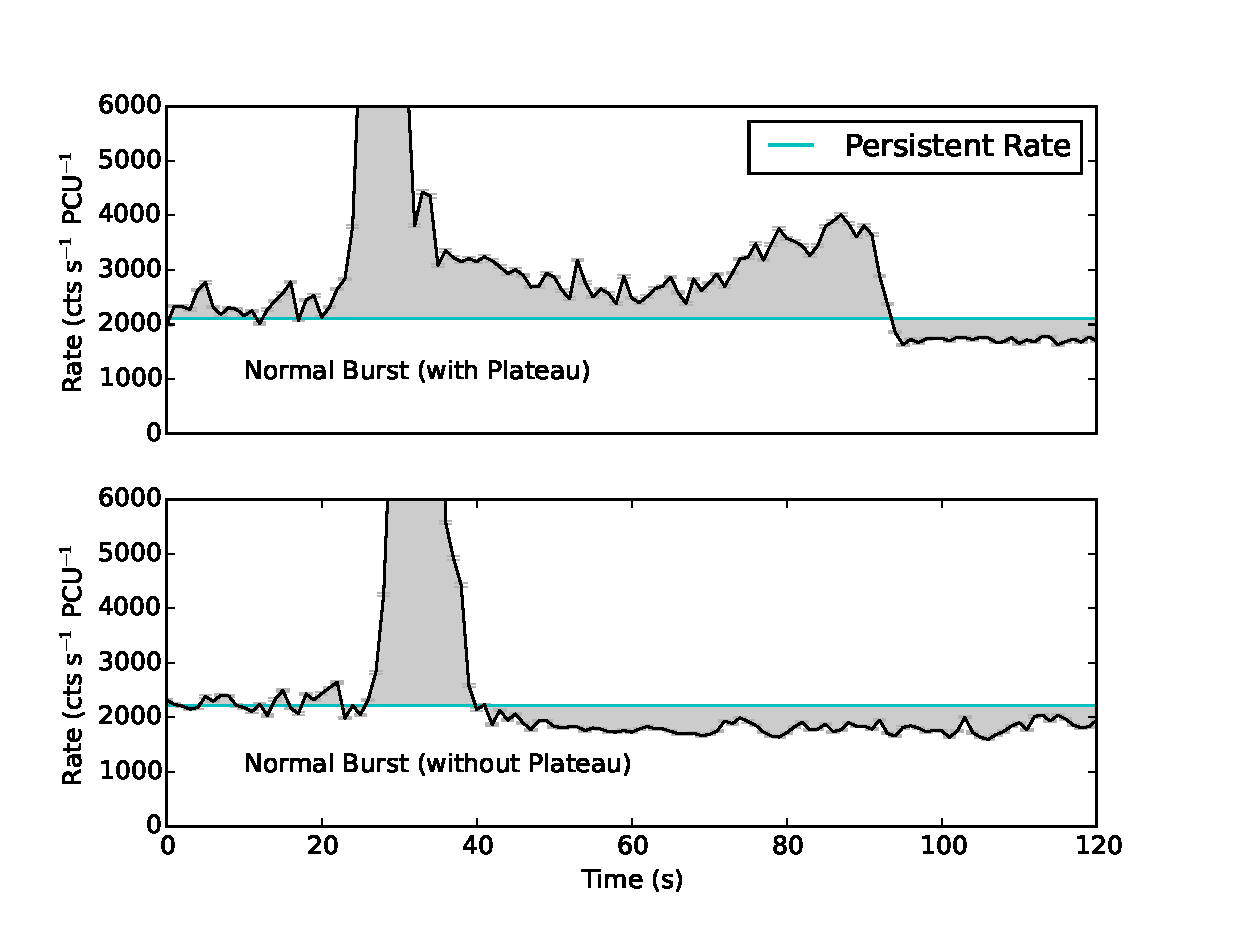
\includegraphics[width=.9\linewidth, trim={0.8cm 0 1.6cm 0},clip]{images/w_woburst.eps}
  \caption[\textit{RXTE} lightcurves of Normal Bursts with (top) and without (bottom) `plateau' features, showing the burst structure in each case.]{\small \indexrxte\textit{RXTE} lightcurves\index{Lightcurve} of Normal Bursts\index{Normal burst} with (top) and without (bottom) `plateau'\index{Plateau} features, showing the burst structure in each case.  The median count rate, which I use as a proxy for the persistent emission\index{Persistent emission}, is plotted in cyan to highlight the presence of the count rate `dip'\index{Dip} after each burst.}
  \label{fig:w_wo}
\end{figure}

\par In order to study Normal Bursts\index{Normal burst}, I fit the burst profiles with phenomenologically-motivated mathematical functions.  In Figure \ref{fig:explain} I show a schematic plot of my model, as well as annotations explaining the identities of the various parameters I use.  I fit the main burst with a skewed Gaussian\index{Gaussian profile}, centred at $t=x_0$ with amplitude $a_b$, standard deviation $\sigma_B$ and skewness\footnote{A measure of how far the peak of the Gaussian is displaced from its centre.} $c$, added to the persistent emission\index{Persistent emission} rate $k$.  I fit the `dip'\index{Dip} with the continuous piecewise function `Dipper function'\index{Dipper function} $f(t)$:

\begin{equation}
f(t)=
\begin{dcases}
k-\frac{a_d(t-t_0)}{d-t_0}, & \text{if } t\leq d\\
k-a_d\exp\left(\frac{d-t}{\lambda}\right), & \text{otherwise}
\end{dcases}
\label{eq:dipper}
\end{equation}

Where $t$ is time, $t_0$ is the start time of the dip\index{Dip}, $a_d$ is the amplitude of the dip, $d$ is the time at the local dip minimum and $\lambda$ is the dip recovery timescale.  This function is based on the finding by \citet{Younes_Expo} that dip count rates recover exponentially, but has the added advantage that the start of the recovery phase can also be fit as an independent parameter.  Using this fit, I can estimate values for burst fluence $\phi_B$, burst scale-length $\sigma_B$, `missing' dip fluence $\phi_D$ and dip scale-length $\lambda$ and compare these with other burst parameters.  When present, I also calculate the fluence of the plateau\index{Plateau} $\phi_p$ by summing the persistent emission\index{Persistent emission}-subtracted counts during the region between the end of the burst (as defined in Section \ref{sec:burst_diff}) and the start of the dip.  For each pair of parameters, I do not consider datapoints when the magnitude of the error on a parameter is greater than the value of the parameter.

\begin{figure}
  \centering
  \includegraphics[width=.9\linewidth, trim={1.9cm 0 2.0cm 0},clip]{images/explainer.eps}
  \caption[A schematic explaining the origin of the 12 Normal Burst parameters used in this study.]{\small A schematic explaining the origin of the 12 Normal Burst\index{Normal burst} parameters used in this study, as well as showing the functional forms of both the skewed Gaussian\index{Gaussian profile} fit to a burst and the `dipper function'\index{Dipper function} (Equation \ref{eq:dipper}) fit to a dip\index{Dip}.  Note that I do not fit a function to the plateau\index{Plateau}, and I calculate its fluence by summing the persistent rate\index{Persistent emission}-subtracted counts.  Diagram is for explanation only and the burst pictured is neither based on real data nor to scale.}
  \label{fig:explain}
\end{figure}

\par I only extract these parameters from Normal Bursts\index{Normal burst} observed by \indexrxte\textit{RXTE} during Outbursts\index{Outburst} 1 \& 2.  This ensures that the resultant parameter distributions I extracted are not affected by differences between instruments.

\subsubsection{Parameter Distributions}

\label{sec:hists}

\par I extracted a total of ten parameters from my fit to each burst\index{Normal burst}: the parameters $a_d$, $d$ and $\lambda$ of the fit to the dip\index{Dip}, the missing fluence $\phi_D$ of the dip, the parameters $a_b$, $\sigma_B$ and $c$ of the skewed Gaussian\index{Gaussian profile} fit to the main burst, the main burst fluence $\phi_B$, the maximum persistent emission-subtracted\index{Persistent emission} rate in the plateau\index{Plateau} $a_p$ and the plateau fluence $\phi_P$.
\par Using my \indexrxte\textit{RXTE} sample of Normal Bursts\index{Normal burst}, I can construct distributions for all of the burst parameters described in Section \ref{sec:struc} for bursts in Outbursts\index{Outburst} 1 \& 2.  I give the mean and standard deviation for each parameter in each outburst in Table \ref{tab:params_perob}, and histograms for each can be found in Appendix \ref{app:hists}.

\begin{table}
\centering
\begin{tabular}{r c c c c c c}
\hline
\hline
 & \multicolumn{2}{c}{\scriptsize Outburst 1} & \multicolumn{2}{c}{\scriptsize Outburst 2} & \multicolumn{2}{c}{\scriptsize Outbursts 1\&2}  \\
 &Mean&S.D.&Mean&S.D.&Mean&S.D.\\
\hline
$\phi_B$&2.74e6&7.8e5&2.25e6&7.6e5&$2.43\mathrm{e}6$&$8.0\mathrm{e}5$\\
$a_B$&3.18e5&8.4e4&2.72e5&9.9e4&$2.90\mathrm{e}5$&$9.6\mathrm{e}4$\\
$\sigma_B$&3.39&0.35&3.42&0.59&3.41&0.52\\
$c$&2.68&1.9&2.79&2.0&2.75&2.0\\
$\phi_d$&1.74e6&1.3e6&1.17e6&3.6e5&$1.38\mathrm{e}6$&$8.7\mathrm{e}5$\\
$a_d$&550&335&536&307&541&318\\
$d$&49&46&20&22&31&36\\
$\lambda$&294&176&229&124&254&150\\
$\phi_p$&1.89e5&2.3e5&7577&5707&1.4e5&1.8e5\\
$a_p$&1289&1113&767&463&1063&928\\
\hline
\hline
\end{tabular}
\caption[A table showing the mean and standard deviation of 10 Normal Burst parameters of \textit{RXTE}-sampled bursts.]{A table showing the mean and standard deviation of 10 Normal Burst\index{Normal burst} parameters of \indexrxte\textit{RXTE}-sampled bursts.  In each case, I give the values for populations from only Outburst\index{Outburst} 1, from only Outburst 2 and from the combined population from both outbursts.  Histograms for each parameter can be found in Appendix \ref{app:hists}.}
\label{tab:params_perob}
\end{table}

\par The mean value of most parameters differs by no more than $\sim50$\% between outbursts\index{Outburst}.  Notable exceptions are $d$, $\phi_p$, $\phi_d$ and $a_p$, which are $\sim2.5$, $\sim2.5$ $\sim1.5$ and $\sim1.7$ times greater in Outburst 1 than in Outburst 2 respectively.  The less significant differences between values of $\phi_B$ and $a_B$ in Outbursts 1 \& 2 are expected, as the amplitude of a burst correlates with persistent rate\index{Persistent emission} $k$ which was generally higher in Outburst 1 than in Outburst 2.

\subsubsection{Correlations}

\label{sec:NormCorr}

\par In total, I extracted 12 parameters for each Normal Burst\index{Normal burst} in my \textit{RXTE} sample: the 10 burst parameters listed in Section \ref{sec:hists}, the recurrence time\index{Recurrence time} $s_t$ until the next burst and the persistent emission\index{Persistent emission} rate $k$ at the time of the burst.
\par As the amplitude of all 3 components in a burst scale with the persistent emission\index{Persistent emission} level, I rescaled my values of $a_b$, $a_d$, $\phi_B$, $\phi_D$ and $\phi_P$ by a factor $\frac{1}{k}$.  I show the covariance matrix with all 66 possible pairings of these normalised parameters in Figure \ref{fig:corr_n} (we present the covariance matrix of these parameters before being rescaled in Appendix \ref{app:corr}).  Using the Spearman's Rank Correlation Coefficient\index{Spearman's rank correlation coefficient}, I find the following $\geq5\,\sigma$ correlations which are highlighted in Figure \ref{fig:corr_n}:

\begin{itemize}
\item Persistent emission\index{Persistent emission} $k$ anticorrelates with normalised burst fluence $\phi_B/k$ ($>10\,\sigma$) and normalised burst amplitude $a_b/k$ ($>10\,\sigma$).
\item Normalised burst fluence $\phi_B/k$ correlates with normalised burst amplitude $a_B/k$ ($8.0\,\sigma$).
\item Normalised dip fluence\index{Dip} $\phi_d/k$ correlates with dip recovery timescale $\lambda$ ($6.3\,\sigma$).
\item Normalised dip amplitude $a_d/k$ anticorrelates with dip falltime $d$ ($5.7\,\sigma$) and dip recovery timescale $\lambda$ ($7.1\,\sigma$).
\item Normalised plateau\index{Plateau} fluence $\phi_p/k$ correlates with normalised plateau amplitude $a_p$ ($6.4\,\sigma$).
\end{itemize}

As $\phi_B$ can be approximated to first order as a product of $a_B$ and $\sigma$, the correlation between $\phi_B$ and $a_B$ is expected as they are not independent parameters.  Similarly, the correlations between $\phi_d$ \& $\lambda$ and $\phi_p$ and $a_p$ are likely due to these pairs of parameters not being independent.

\begin{figure}
  \centering
  \includegraphics[width=\linewidth, trim={2.1cm 2cm 3.5cm 3cm},clip]{images/corrplot_normed.eps}
  \caption[Covariance Matrix with a scatter plot of each pairing of the 12 normalised Normal Burst parameters listed in section \ref{sec:NormCorr}.]{\small Covariance Matrix with a scatter plot of each of the 66 pairings of the 12 Normal Burst\index{Normal burst} parameters listed in section \ref{sec:NormCorr}.  Amplitudes and fluences have been normalised by dividing by the persistent emission\index{Persistent emission} rate $k$.  Pairings which show a correlation using the Spearman Rank\index{Spearman's rank correlation coefficient} metric with a significance $\geq5\,\sigma$ are highlighted in red.}
  \label{fig:corr_n}
\end{figure}

\subsubsection{Colour Evolution}

\par To explore the spectral\index{Spectroscopy} behaviour of Normal Bursts\index{Normal burst}, Toyah Overton (\textsf{T.O.}) and I studied the evolution of the hardness\index{Colour} (the ratio between count rate in the energy bands $\sim2$--$7$ and $\sim8$--$60$\,keV energy bands) as a function of count rate during the individual bursts.  Plotting hardness-intensity diagrams\index{Hardness-intensity diagram} allow us to check for spectral evolution in a model-independent way.  We do not correct them for background\index{Background subtraction} as the count rates in both bands are very high.
\par \textsf{T.O.} and I find evidence of hysteretic\index{Hysteresis} loops in hardness-intensity\index{Hardness-intensity diagram} space in some, but not all, of the Normal Bursts\index{Normal burst} in my sample; see Figure \ref{fig:loop} for an example of such a loop.  The existence of such a loop suggests significant spectral\index{Spectroscopy} evolution throughout the burst.  This finding can be contrasted with results from previous studies in different energy bands (e.g. \citealp{Woods_OB2} from $\sim25$--100\,keV) which suggested no spectral evolution during Type II bursts\index{X-ray burst!Type II} in this source.

\begin{figure}
  \centering
  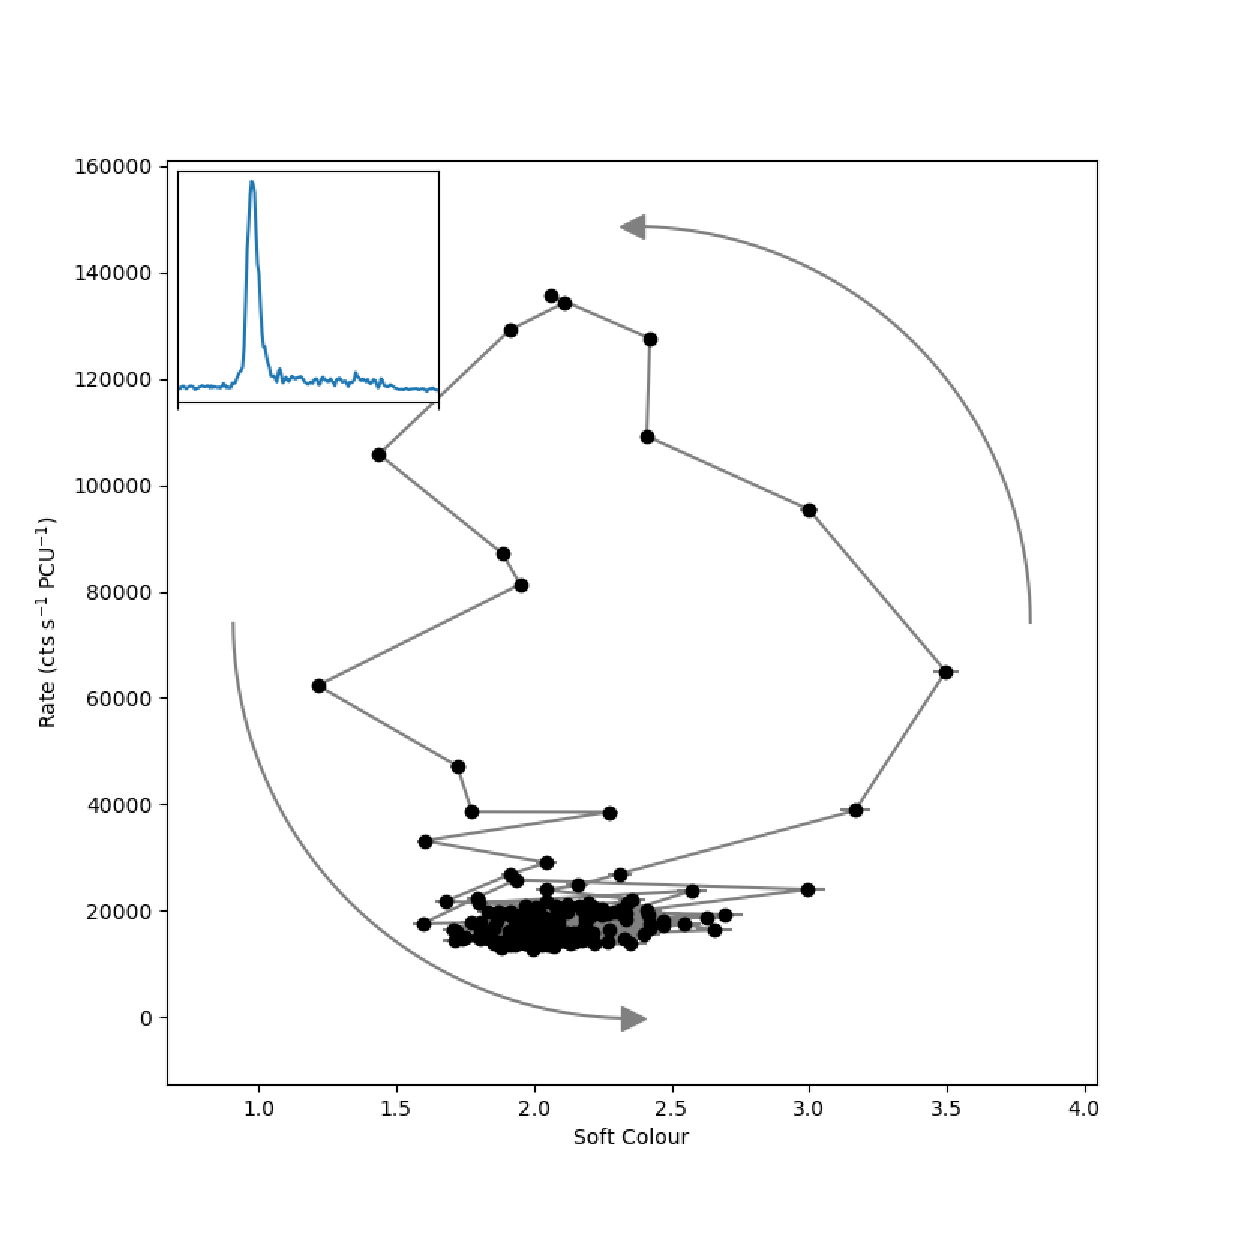
\includegraphics[width=.9\linewidth, trim={0.4cm 1cm 1.1cm 1cm},clip]{images/Loop1.eps}
  \caption[A hardness-intensity diagram of a typical Normal Burst.]{\small A 1\,s-binned hardness-intensity diagram\index{Hardness-intensity diagram} of a Normal Burst\index{Normal burst} from \indexpca\textit{RXTE}/PCA observation 10401-01-08-00, with an inset 2--60\,keV lightcurve\index{Lightcurve}.  Significant colour\index{Colour} evolution can be seen during the burst, taking the form of a loop\index{Hysteresis}.}
  \label{fig:loop}
\end{figure}

\subsection{Minibursts}

\label{sec:Minibursts}

\par I define Minibursts\index{Miniburst} as the set of all bursts\index{X-ray burst} with a peak 1\,s binned \indexpca\textit{RXTE}/PCA-equivalent count rate of $<300\%$ of the persistent rate\index{Persistent emission}.  Minibursts account for 48 out of the 190 bursts identified for this study.  They are observed during all 3 Outbursts\index{Outburst}, and occur during the same times that Normal Bursts\index{Normal burst} are present.  Minibursts occurred between MJDs 50117 and 50200 in Outburst 1, and between 50466 and 50542 in Outburst 2; during these intervals, \indexrxte\textit{RXTE} observed the source for a total of 192\,ks.  These intervals correspond to the times between the peak of each outburst and and the time that the persistent intensity falls below $\sim0.1$\,Crab.

\subsubsection{Recurrence Time}

\par There are only 10 observations with \indexrxte\textit{RXTE} which contain multiple Minibursts\index{Miniburst}.  Using these, I find minimum and maximum Miniburst recurrence\index{Recurrence time} times of 116 and 1230\,s.
\par I find 17 \indexrxte\textit{RXTE} observations which contain both a Miniburst\index{Miniburst} and a preceding Normal Burst\index{Normal burst}, and find minimum and maximum Normal Burst $\rightarrow$ Miniburst recurrence times\index{Recurrence time} of 461 and 1801\,s.

\subsubsection{Structure}

\par In Figure \ref{fig:a_mini}, I show the lightcurve\index{Lightcurve} of a representative Miniburst\index{Miniburst}, and I show all Minibursts overplotted on each other in Figure \ref{fig:mini_over}.  These bursts are roughly Gaussian\index{Gaussian profile} in shape with a large variation in peak count rate; as can be seen in Figure \ref{fig:mini_over}, however, the persistent\index{Persistent emission}-normalised peak count rates of Minibursts are all roughly consistent with 2.

\begin{figure}
  \centering
  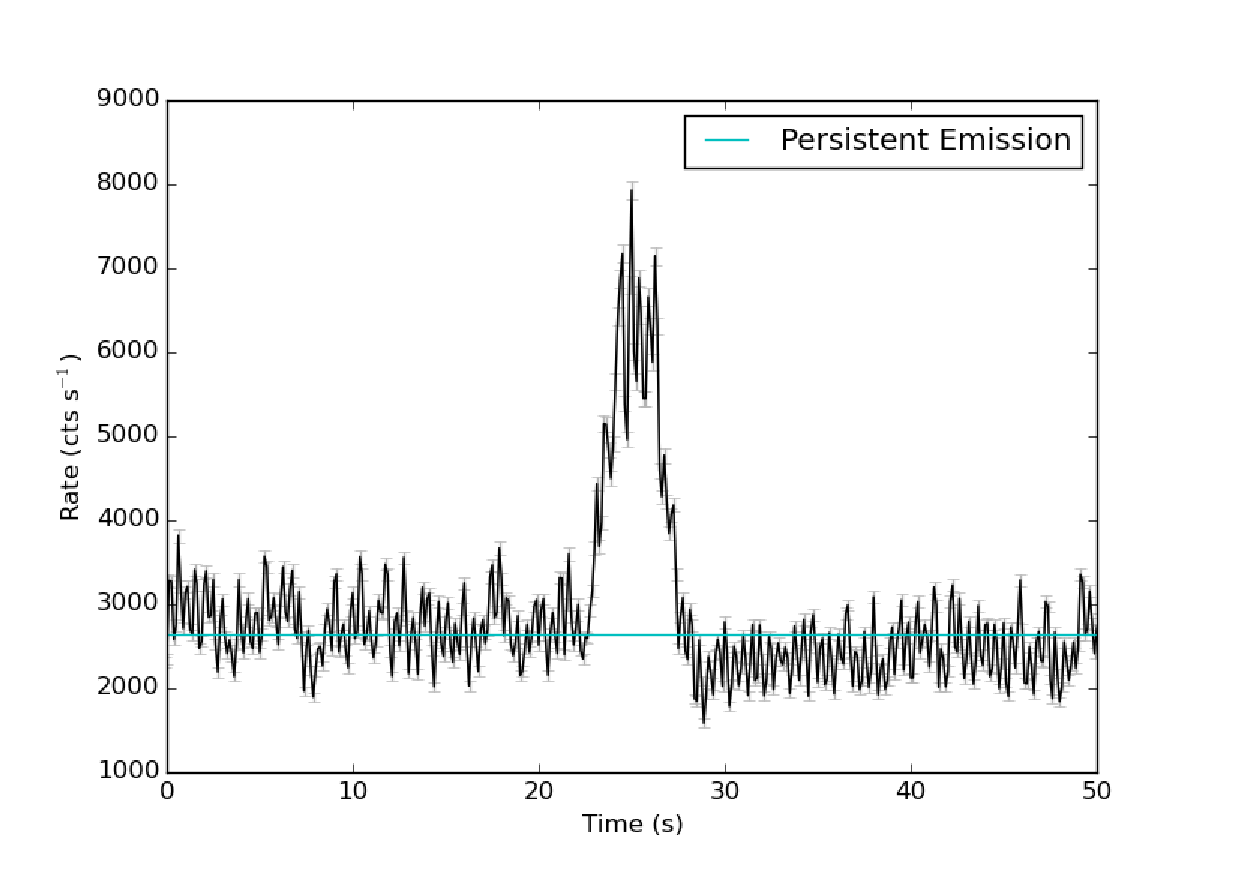
\includegraphics[width=.9\linewidth, trim={0cm 0 0cm 0},clip]{images/mini.eps}
  \caption[A representative \textit{RXTE} lightcurve of a Miniburst.]{\small  A representative \indexpca\textit{RXTE}/PCA lightcurve\index{Lightcurve} of a Miniburst\index{Miniburst} from OBSID 20077-01-03-00 in Outburst\index{Outburst} 2.}
  \label{fig:a_mini}
\end{figure}
\begin{figure}
  \centering
  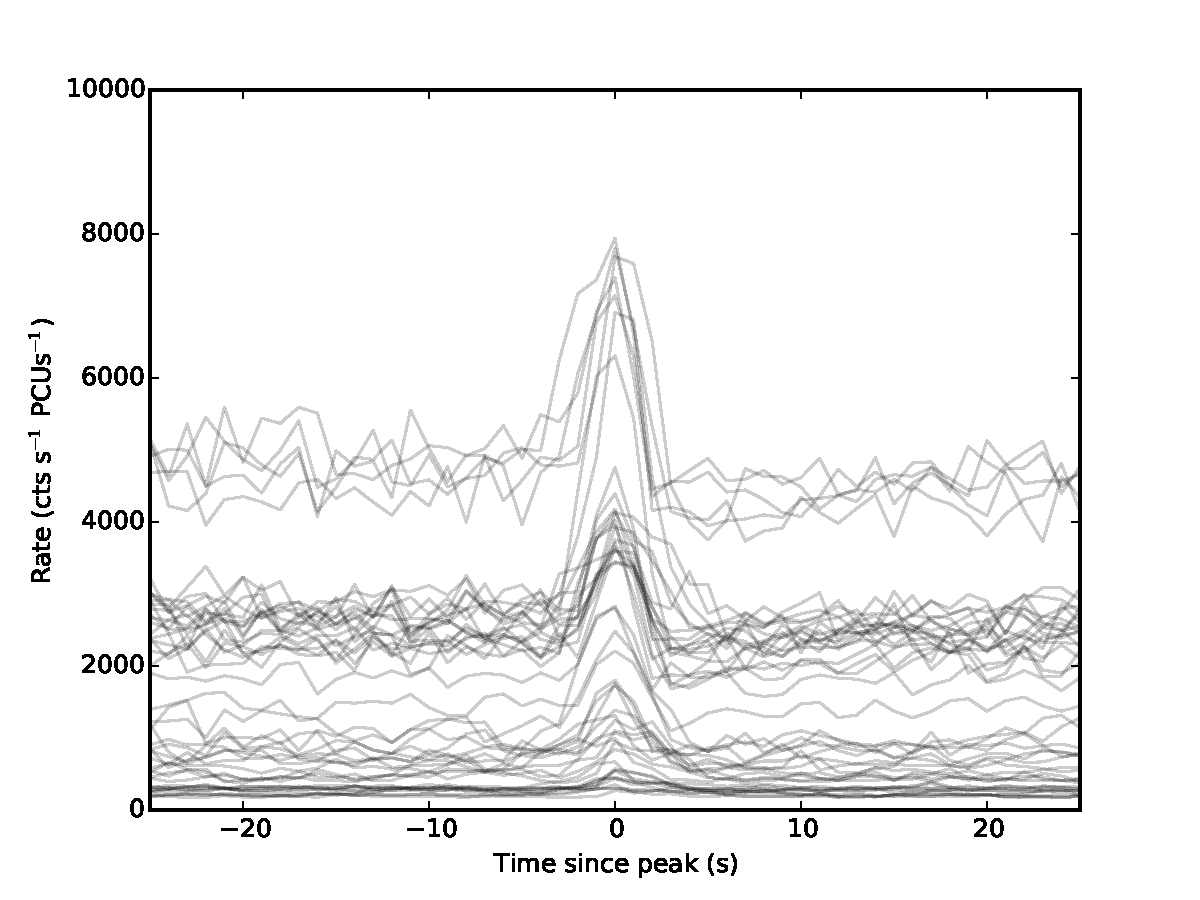
\includegraphics[width=.9\linewidth, trim={0.4cm 0 1.1cm 0},clip]{images/1000mini.pdf}
  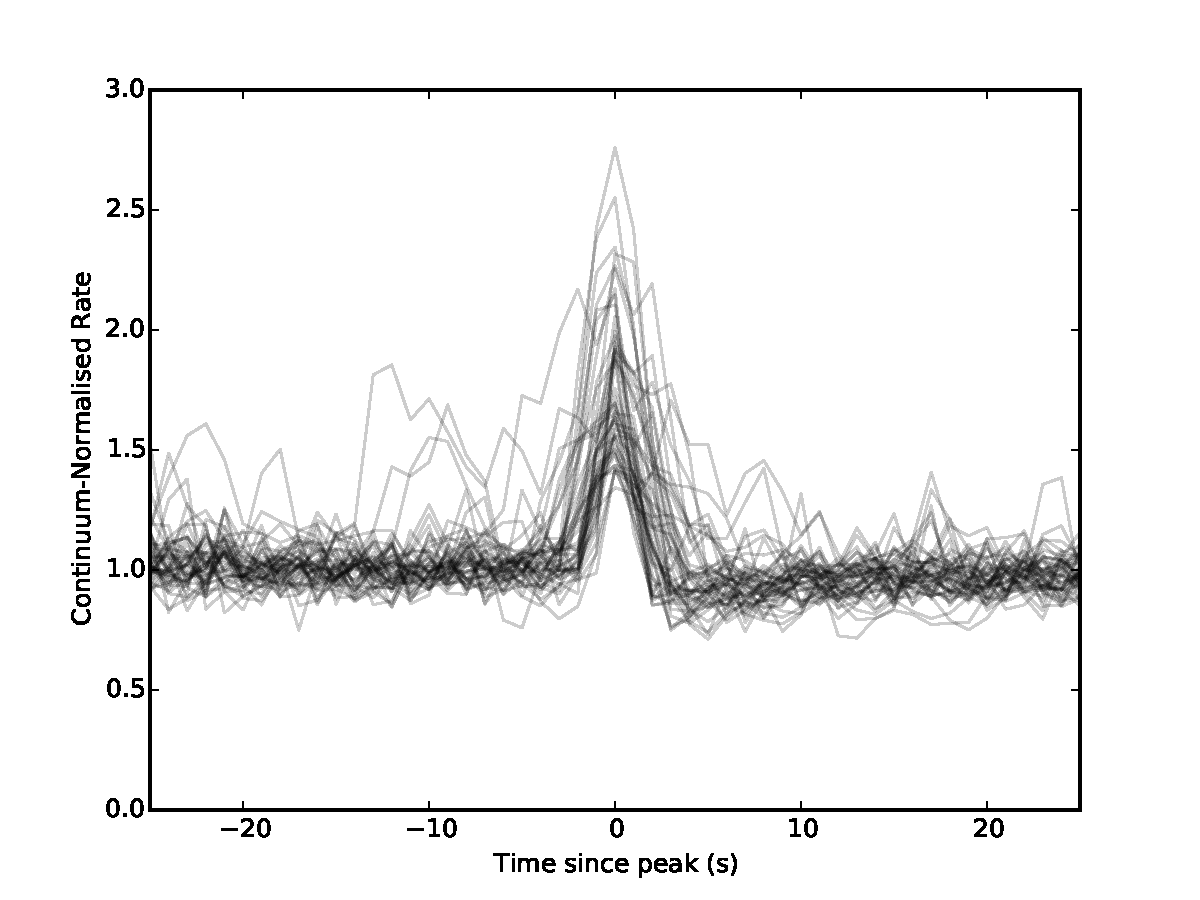
\includegraphics[width=.9\linewidth, trim={0.4cm 0 1.1cm 0},clip]{images/1000mini_renormed.pdf}
  \caption[A plot of every Miniburst, centred by the time of its peak, overlaid on top of each other.]{\small  \textbf{Top:} a plot of every Miniburst\index{Miniburst}, centred by the time of its peak, overlaid on top of each other.  \textbf{Bottom:} a plot of every Miniburst in which count rates have been normalised by the persistent emission\index{Persistent emission} count rate during the observation from which each burst was observed.}
  \label{fig:mini_over}
\end{figure}

\par Minibursts\index{Miniburst} are all $\sim5$\,s in duration, and some show signs of a `dip'\index{Dip} feature similar to those seen in Normal Bursts\index{Normal burst}.  I find that the timescales of these dips are all $\lesssim10$\,s.  I estimate `missing' fluence in each dip by integrating the total persistent-rate\index{Persistent emission}-subtracted counts between the end of the burst and a point 10\,s later.  If this `missing fluence' is less than half of the standard deviation in count rate multiplied by 5\,s, which represents the smallest $<10$\,s triangle-shaped dip which would be detectable above noise in a given dataset, I treat the dip in that outburst as not being detected.
\par Due to the relatively short duration and low amplitudes of Minibursts\index{Miniburst}, I am unable to reliably discern whether they contain a single peak or multiple peaks.  For this reason I do not fit them mathematically.

\subsubsection{Parameters \& Correlations}

\label{sec:ministruc}

\par For each Miniburst\index{Miniburst}, I extract the following parameters:

\begin{itemize}
\item Total burst fluence and burst fluence divided by persistent emission\index{Persistent emission}.
\item Peak 1\,s binned rate and peak rate divided by persistent emission.
\item Rise time, fall time and total time.
\end{itemize}
The mean and standard deviation of each of these parameters, calculated from \indexrxte\textit{RXTE} data, is presented in Table \ref{tab:mini_param} for Outburst\index{Outburst} 1, Outburst 2 and the combined population of Minibursts from Outbursts 1 \& 2.  The standard deviations on the fluence and peak rates of Minibursts are very large, suggesting that these parameters are distributed broadly.

\begin{table}
\centering
\begin{tabular}{r c c c c c c}
\hline
\hline
 & \multicolumn{2}{c}{\scriptsize Outburst 1} & \multicolumn{2}{c}{\scriptsize Outburst 2} & \multicolumn{2}{c}{\scriptsize Outbursts 1\&2}  \\
 &Mean&S.D.&Mean&S.D.&Mean&S.D.\\
\hline
\scriptsize Fluence&6792&5776&4474&3307&5422&4627\\
\scriptsize Peak Rate&3501&2851&2473&1664&2902&2293\\
\scriptsize Fluence/$k$&3.67&1.13&3.58&1.47&3.61&1.34\\
\scriptsize Peak Rate/$k$&1.90&0.37&1.76&0.28&1.82&0.32\\
\scriptsize Rise Time&2.33&0.8&2.03&1.1&2.15&1.0\\
\scriptsize Fall Time&2.32&0.9&2.35&1.0&2.32&0.9\\
\scriptsize Tot. Time&4.61&1.0&4.38&01.0&4.47&1.0\\
\hline
\hline
\end{tabular}
\caption[A table showing the mean and standard deviation of 7 parameters of \textit{RXTE}-sampled Minibursts from the 1996 outburst, the 1997 outburst and both outbursts combined.]{A table showing the mean and standard deviation of 7 parameters of \indexrxte\textit{RXTE}-sampled Minibursts\index{Miniburst} from Outburst\index{Outburst} 1, Outburst 2 and both outbursts combined.  Fluence is given in cts\,PCU$^{-1}$, peak rate is given in cts\,s$^{-1}$\,PCU$^{-1}$ and rise, fall and total time are given in s.  $k$ is the persistent emission\index{Persistent emission} rate during the observation in which a given burst was detected.}
\label{tab:mini_param}
\end{table}

\par Using the Spearman's Rank\index{Spearman's rank correlation coefficient} metric, I find only two correlations above the 5$\,\sigma$ level:
\begin{itemize}
\item Fluence is correlated with peak rate ($7.3\,\sigma$).
\item Fluence divided by persistent rate\index{Persistent emission} is correlated with peak rate divided by persistent rate ($7.1\,\sigma$).
\end{itemize}
As in Normal Bursts\index{Normal burst}, a correlation between peak rate and fluence is to be expected.  However, due to the poor statstics associated with Miniburst\index{Miniburst} parameters, it is likely that other parameter pairs are also correlated.

\subsubsection{Colour Evolution}

\par Minibursts\index{Miniburst} show the greatest magnitude of evolution in colour\index{Colour} of all the classes of burst\index{X-ray burst}.  In Figure \ref{fig:minihard}, I show how the hardness ratio between the 4--10 and 2--4\,keV energy bands changes during an observation containing both a Miniburst and a Normal Burst\index{Normal burst}.  I find that the hardness ratio increases by $\sim50\%$ in a Miniburst, significantly more than the change in hardness during Normal or Mesobursts\index{Mesoburst}.  The statistics in minibursts were too poor to check for the presence of hysteresis\index{Hysteresis}.

\begin{figure}
  \centering
  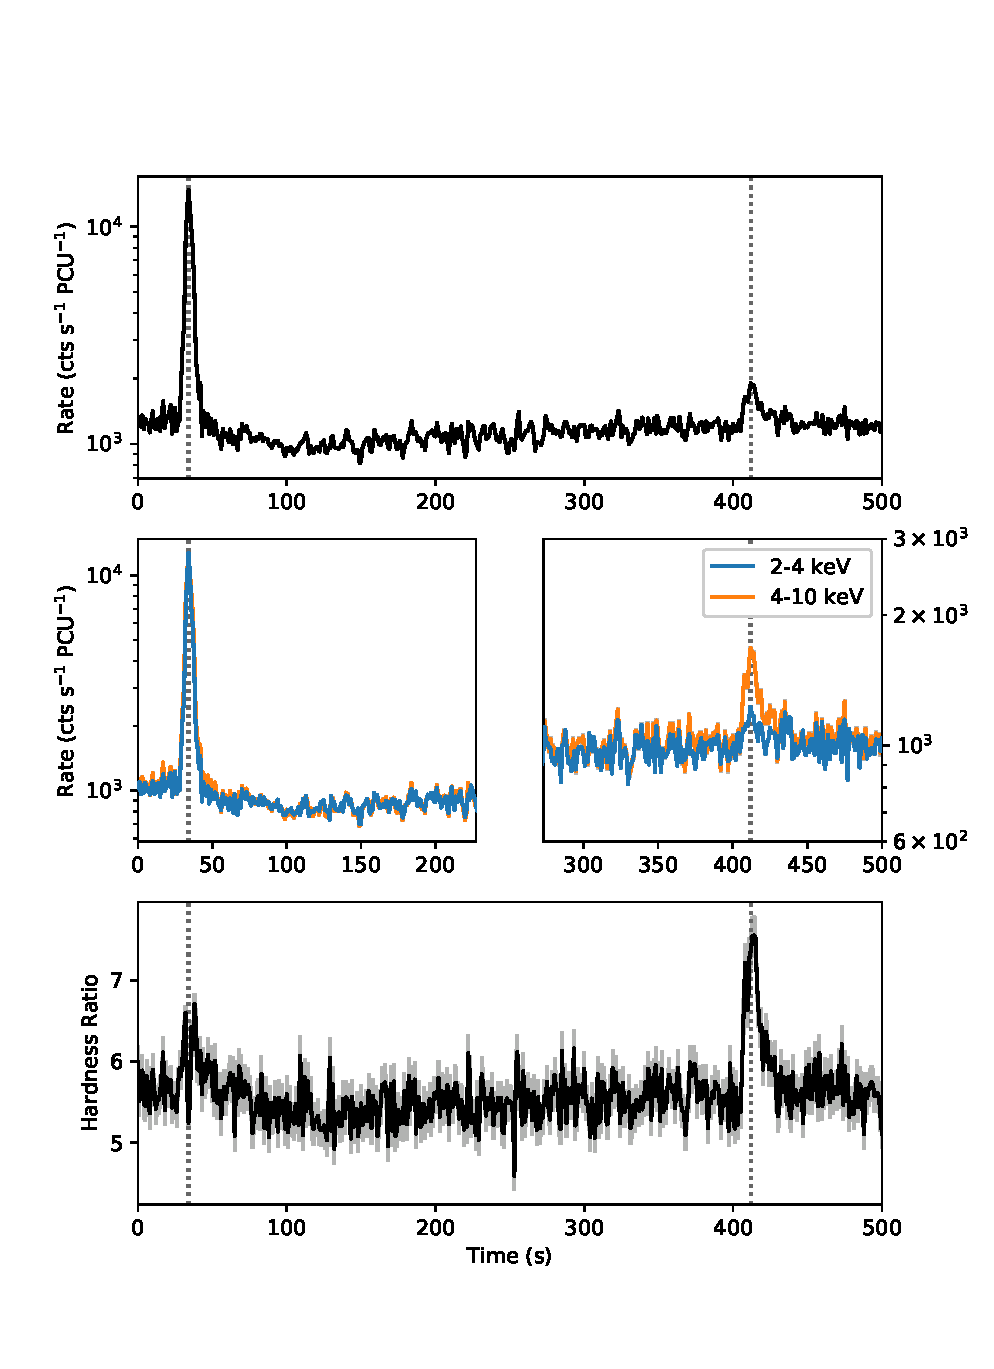
\includegraphics[width=.9\linewidth, trim={0.7cm 1.4cm 0.2cm 1.4cm},clip]{images/hardness_mini.eps}
  \caption[A portion of observation 10401-01-16-00, featuring a fNormal Burst and a Miniburst.]{\small A portion of observation 10401-01-16-00, featuring a Normal Burst\index{Normal burst} ($\sim30$\,s) and a Miniburst\index{Miniburst} ($\sim410$\,s).  The top panel shows the total 2--10\,keV lightcurve\index{Lightcurve}.  The middle panel shows lightcurves from two different energy bands; the count rates from the soft energy band have been multiplied by 5.4 so they can more easily be compared with the hard energy band.  The bottom panel shows the evolution over time of the ratio\index{Colour} between the rates in the two bands.   As can be seen in panels 2 and 3, the Miniburst has a significantly higher fractional amplitude in the 4--10\,keV energy band than in the 2--4\,keV band.}
  \label{fig:minihard}
\end{figure}

\subsection{Mesobursts}

\par I define Mesobursts\index{Mesoburst} as the set of all bursts\index{X-ray burst} with a persistent-emission\index{Persistent emission}-subtracted peak 1\,s binned \indexpca\textit{RXTE}/PCA-equivalent count rate below 3000\,cts\,s$^{-1}$\,PCU$^{-1}$ in which the peak of the burst reaches at least $300\%$ of the persistent rate.  Mesobursts account for 43 out of the 190 bursts identified for this study.  They are observed in \indexrxte\textit{RXTE} data from both Outbursts\index{Outburst} 1 \& 2; in both cases they occur after the main outburst and before or during a rebrightening\index{Re-flare} event.  Mesobursts occurred between MJDs 50238 and 50248 in Outburst 1, and between 50562 and 50577 in Outburst 2; during these intervals, \textit{RXTE} observed the source for a total of 44\,ks.  As no soft X-ray instrument monitored the Bursting Pulsar during the latter stages of Outburst 3, it is unclear whether Mesobursts occurred during this outburst.  The one pointed observation of \indexnustar\textit{NuSTAR} made during this time did not detect any Mesobursts.

\subsubsection{Recurrence Time}

\par Only 6 \indexrxte\textit{RXTE} observations in Outburst\index{Outburst} 1, and 4 in Outburst 2, contain multiple Mesobursts\index{Mesoburst}.  From my limited sample I find minimum and maximum recurrence\index{Recurrence time} times of $\sim230$ and $\sim1550$\,s in Outburst 1 and minimum and maximum recurrence times of $\sim310$ and $\sim2280$\,s in Outburst 2.

\subsubsection{Structure}

\par The structure of the main part of a Mesoburst\index{Mesoburst} is significantly more complex than in Normal Bursts\index{Normal burst}, consisting of a large number of secondary peaks near the main peak of the burst.  Mesobursts never show the post-burst `dip'\index{Dip} feature that we see in Normal Bursts or Minibursts\index{Miniburst}, but they can show `plateaus'\index{Plateau}.  In Figure \ref{fig:mesoplateau} I show an example of a Mesoburst with a plateau similar to those seen after Normal Bursts, suggesting a connection between the two classes.

\begin{figure}
  \centering
  \includegraphics[width=.9\linewidth, trim={0.4cm 0 1.1cm 0},clip]{images/mesoplat.eps}
  \caption[A lightcurve from \textit{RXTE} observation 20078-01-17-00 from Outburst 2, showing an apparent `plateau' feature after a Mesoburst.]{\small A \index{Lightcurve}lightcurve from \indexpca\textit{RXTE}/PCA observation 20078-01-17-00 from Outburst\index{Outburst} 2, showing an apparent `plateau'\index{Plateau} feature after a Mesoburst\index{Mesoburst}.}
  \label{fig:mesoplateau}
\end{figure}

\par In Figure \ref{fig:meso_over} I show the lightcurves\index{Lightcurve} of all Mesobursts\index{Mesoburst} observed by \indexrxte\textit{RXTE} overlayed on top of each other before (top panel) and after (bottom panel) being renormalised by persistent emission\index{Persistent emission} rate.  It can be seen that the intensity and structure of these bursts is much more variable than in Normal Bursts\index{Normal burst} (see Figure \ref{fig:norm_overlay}).  However, each Mesoburst has a fast rise followed by a slow decay, and they occur over similar timescales of $\sim10$--$30$\,s.

\begin{figure}
  \centering
  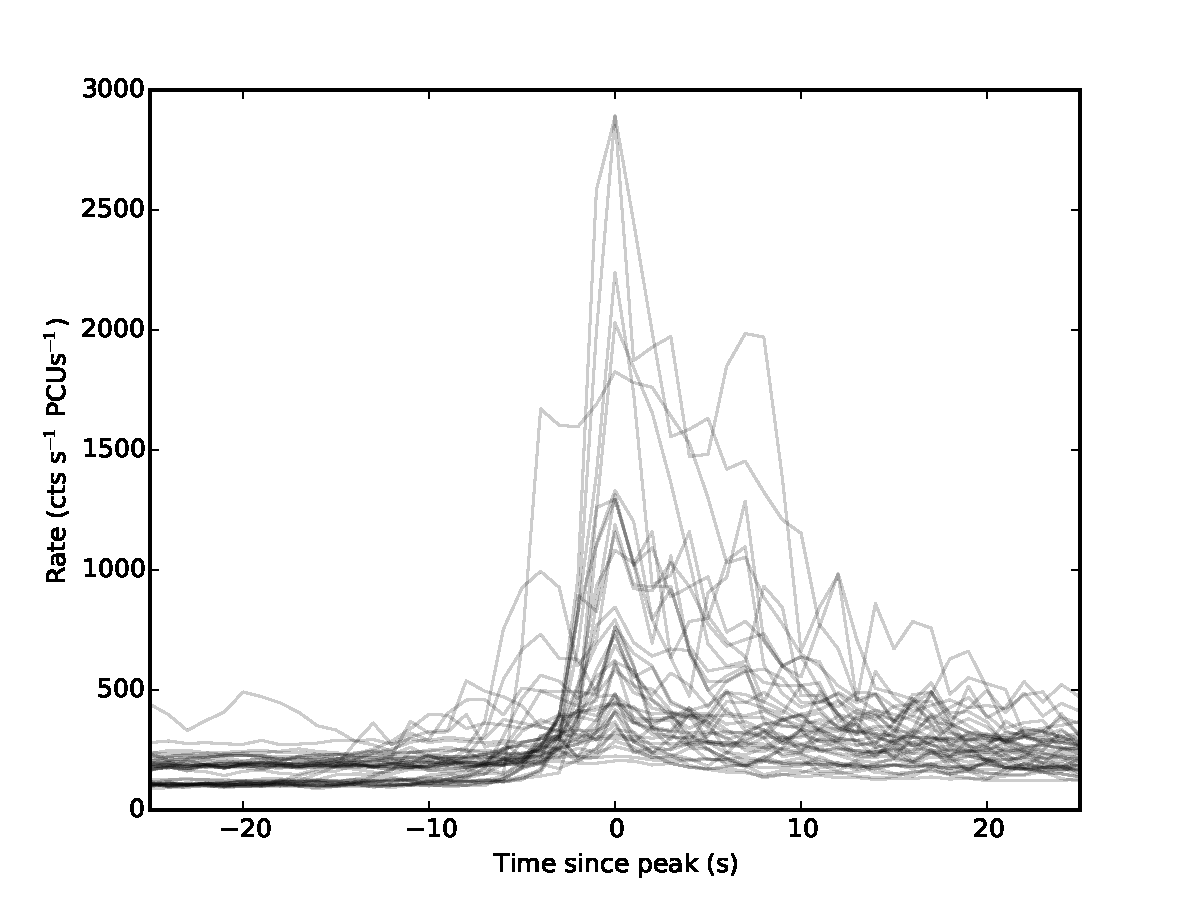
\includegraphics[width=.9\linewidth, trim={0.4cm 0 1.1cm 0},clip]{images/1000meso.pdf}
  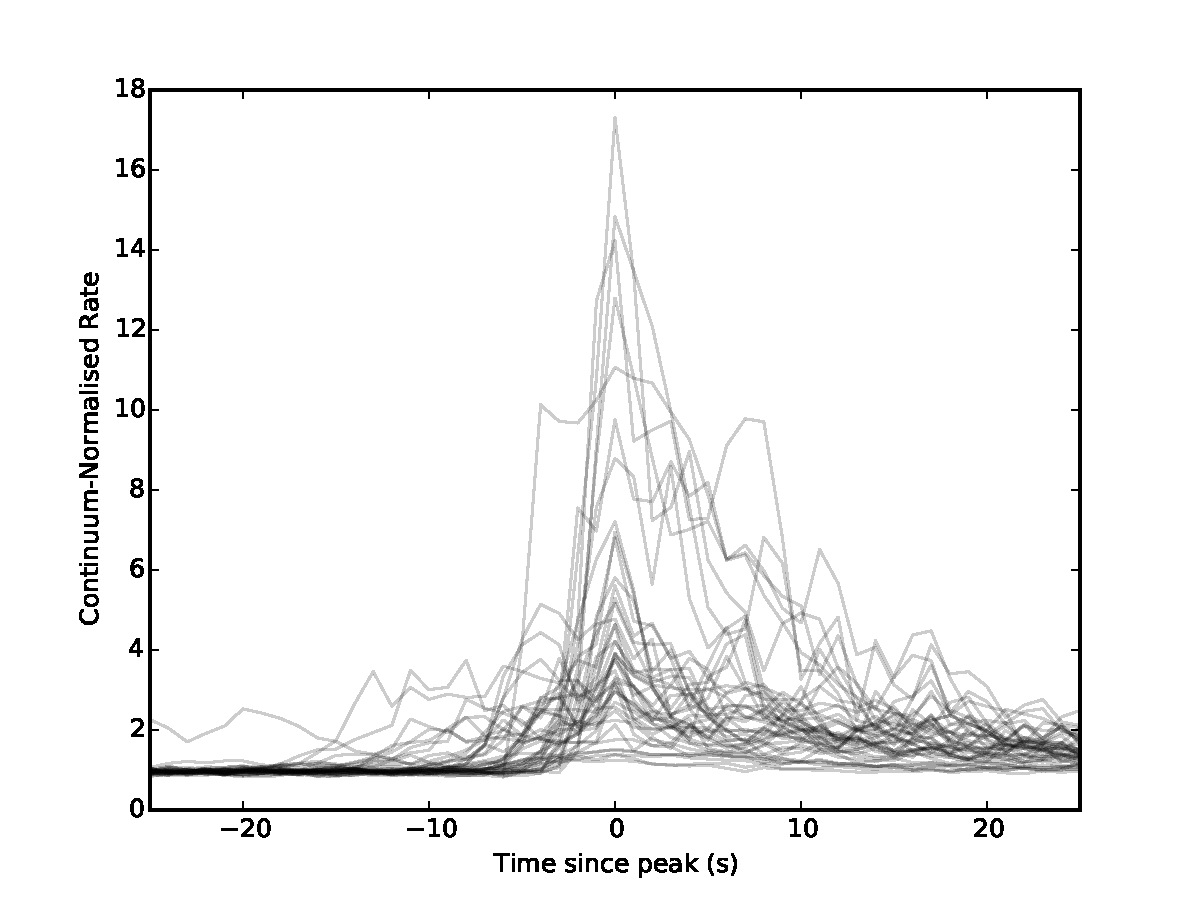
\includegraphics[width=.9\linewidth, trim={0.4cm 0 1.1cm 0},clip]{images/1000meso_renormed.pdf}
  \caption[A plot of every Mesoburst, centred by the time of its peak, overlaid on top of each other.]{\small  \textbf{Top:} a lightcurve\index{Lightcurve} of every Mesoburst\index{Mesoburst}, centred by the time of its peak, overlaid on top of each other.  \textbf{Bottom:} a plot of every Mesoburst in which count rates have been normalised by the persistent emission\index{Persistent emission} count rate during the observation from which each burst was observed.}
  \label{fig:meso_over}
\end{figure}

\subsubsection{Parameters \& Correlations}

\label{sec:mesostruc}

\par Due to the complexity structure of Mesobursts\index{Mesoburst}, I do not fit them mathematically as I did for Normal Bursts\index{Normal burst}.  Instead I extract the same parameters as for Minibursts\index{Miniburst} (see the list in Section \ref{sec:ministruc}).  The mean and standard deviation of each of these parameters, calculated from \indexpca\textit{RXTE}/PCA data, is presented in Table \ref{tab:meso_param}.  Due to the relative low number of Mesobursts compared to Normal Bursts, I only present the results from the combined set of bursts in both Outbursts\index{Outburst} 1 \& 2.  In general, Mesobursts are longer in duration than Normal Bursts, and have significantly smaller amplitudes and fluences (compare e.g. Table \ref{tab:params_perob}).

\begin{table}
\centering
\begin{tabular}{l c c}
\hline
\hline
&Mean&Standard Deviation\\
\hline
Fluence \scriptsize(cts\,PCU$^{-1}$)&6067&6707\\
Peak Rate \scriptsize(cts\,s$^{-1}$\,PCU$^{-1}$)&665.4&658.4\\
Fluence/$k$&48.6&32.8\\
Peak Rate/$k$&5.32&4.0\\
Rise Time \scriptsize(s)&6.95&4.9\\
Fall Time \scriptsize(s)&18.28&10.8\\
Total Time \scriptsize(s)&25.88&13.3\\
\hline
\hline
\end{tabular}
\caption[A table showing the mean and standard deviation of 7 burst parameters of \textit{RXTE}-sampled Mesobursts from the 1996 \& 1997 outbursts.]{A table showing the mean and standard deviation of 7 burst parameters of \indexrxte\textit{RXTE}-sampled Mesobursts\index{Mesoburst} from Outbursts\index{Outburst} 1 \& 2.  $k$ is the persistent emission\index{Persistent emission} rate during the observation in which a given burst was detected.}
\label{tab:meso_param}
\end{table}

\par Using the Spearman's Rank metric\index{Spearman's rank correlation coefficient}, I find a number correlations above the 5$\,\sigma$ level:
\begin{itemize}
\item Fluence is correlated with peak rate ($>10\,\sigma$), peak rate divided by persistent rate\index{Persistent emission} ($6.7\,\sigma$), fall time ($6.8\,\sigma$) and total time ($6.0\,\sigma$).
\item Fluence divided by persistent rate is correlated with peak rate divided by persistent rate ($7.3\,\sigma$).
\item Peak rate is also correlated with peak rate divided by persistent rate ($7.4\,\sigma$), fall time ($5.8\,\sigma$) and persistent level ($6.2\,\sigma$).
\item Rise time correlates with total time ($5.4\,\sigma$).
\item Fall time correlates with total time ($>10\,\sigma$).
\end{itemize}

Again, the correlation between fluence and peak rate is expected, as is the correlation between peak rate and peak rate divided by persistent rate.

\subsubsection{Colour Evolution}

\par The hardness ratio\index{Colour} of the emission from the source decreases significantly during Mesobursts\index{Mesoburst}, with the PCA\indexpca\ 8--60/2--7\,keV colour decreases from $\sim0.6$ between bursts to $\sim0.2$ at the peak of a burst.  Due to the poor statistics of these features compared with Normal Bursts\index{Normal burst}, I was unable to check for evidence of hardness-intensity hysteresis\index{Hardness-intensity diagram}.

\subsection{Structured `Bursts'}

\par I define Structured Burst\index{Structured bursting} observations as observations in which the recurrence time\index{Recurrence time} between bursts\index{X-ray burst} is less than, or approximately the same as, the duration of a single burst.  Structured Bursts constitute the most complex behaviour I find in my dataset.  Unlike the other classes of burst \textsf{A.A.} and I identify, Structured Bursts are not easily described as discrete phenomena.  I find Structured Bursts in 54 observations which are listed in Appendix \ref{app:obs}.
\par In both outbursts\index{Outburst} covered by \indexrxte\textit{RXTE}, Structured Bursts occur\index{Structured bursting} in the time between the end of the main outburst and the start of a rebrightening\index{Re-flare} event.  In both cases these periods of Structured Bursts are preceded by a period populated by Mesobursts\index{Mesoburst}.  Mesobursts occurred between MJDs 50248 and 50261 in Outburst 1, and between 50577 and 50618 in Outburst 2; during these intervals, \textit{RXTE} observed the source for a total of 81\,ks.  Notably, as I show in Figure \ref{fig:meso_in_struc}, one Outburst 1 \textit{RXTE} lightcurve containing Structured Bursting also contains a bright Mesoburst.

\begin{figure}
  \centering
  \includegraphics[width=.9\linewidth, trim={0.4cm 0 1.1cm 0},clip]{images/meso_in_struc.eps}
  \caption[A lightcurve from \textit{RXTE}/PCA observation 10401-01-57-03, showing a Mesoburst occuring during a period of Structured Bursting.]{\small A lightcurve\index{Lightcurve} from \indexpca\textit{RXTE}/PCA observation 10401-01-57-03, showing a Mesoburst\index{Mesoburst} occuring during a period of Structured Bursting\index{Structured bursting}.}
  \label{fig:meso_in_struc}
\end{figure}

\par In both outbursts\index{Outburst}, the amplitude of Structured Bursting\index{Structured bursting} behaviour decreases as the outburst\index{Outburst} approaches the peak of the rebrightening\index{Re-flare} event.  This amplitude continues to decrease as the Structured Burst behaviour evolves into the low-amplitude noisy variability\index{Variability} associated with the source's evolution towards the low/hard state\index{Low/Hard state}.

\subsubsection{Colour Evolution}

\par I produce hardness-intensity diagrams\index{Hardness-intensity diagram} for a number of Structured Bursting\index{Structured bursting} observations; I show a representative example in Figure \ref{fig:struc_hard}.  I find that hardness\index{Colour} is strongly correlated with count rate during this class of bursting, but that the magnitude of the change in hardness is no greater than $\sim30\%$.  This is less than the change in hardness that I find during Normal\index{Normal burst} or Minibursts\index{Miniburst}.  I also find no evidence of hysteretic\index{Hysteresis} hardness-intensity loops from Structured Bursts.

\begin{figure}
  \centering
  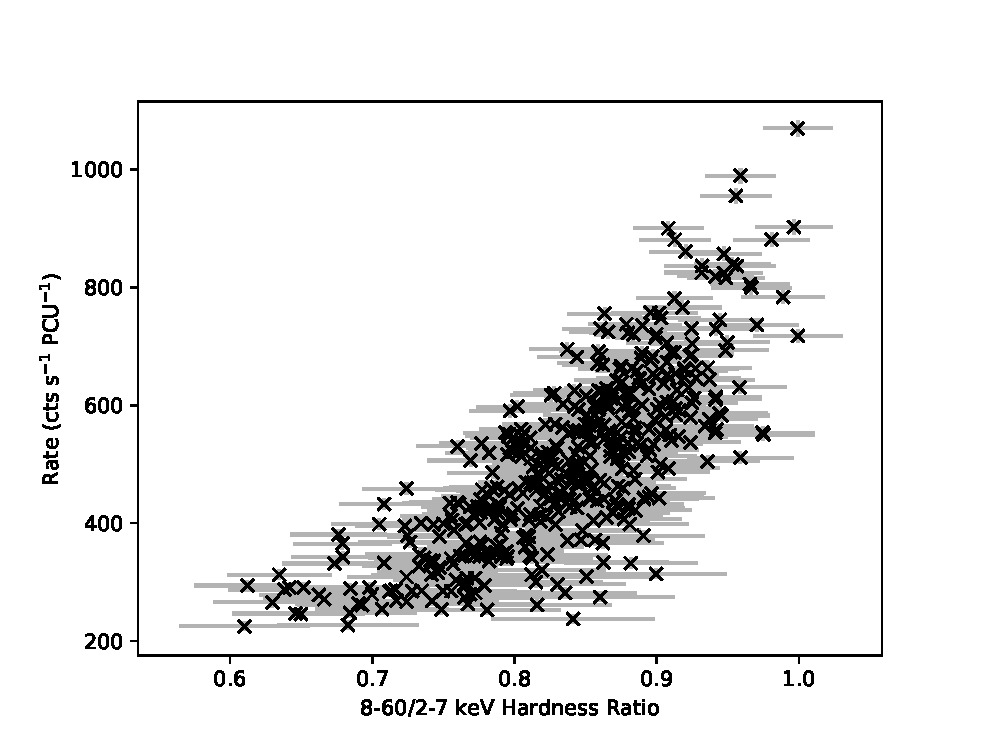
\includegraphics[width=.9\linewidth, trim={0.4cm 0 1.cm 0},clip]{images/struc_hard.eps}
  \caption[A hardness-intensity diagram from \textit{RXTE} observation 20078-01-23-00, showing that hardness tends to correlate with intensity during Structured Bursting.]{\small A 1\,s-binned hardness-intensity diagram\index{Hardness-intensity diagram} from \indexrxte\textit{RXTE} observation 20078-01-23-00, showing that hardness\index{Colour} tends to correlate with intensity during Structured Bursting\index{Structured bursting}.  Data are binned to 8\,s, and background\index{Background subtraction} has been estimated by subtracting mean count rates in the relevant energy bands from \textit{RXTE} OBSID 30075-01-26-00.}
  \label{fig:struc_hard}
\end{figure}

\subsubsection{Types of Structured Bursting}
\label{sec:struc_var}

\par In Figure \ref{fig:Types_Struc}, I present a selection of lightcurves\index{Lightcurve} which show the different types of variability\index{Variability} that can be seen during periods of Structured Bursting\index{Structured bursting}.  These consist of a variety of patterns of flares\index{Flare} and flat-bottomed dips\index{Dip}, and both \indexrxte\textit{RXTE}-observed outbursts\index{Outburst} show several of these different patterns of Structured Bursting.  As all types of Structured Bursting have similar amplitudes and occur in the same part of each outburst, I consider them to be generated by the same physical process.  I do not seperate these patterns into separate subclasses in this thesis.

\begin{figure}
  \centering
  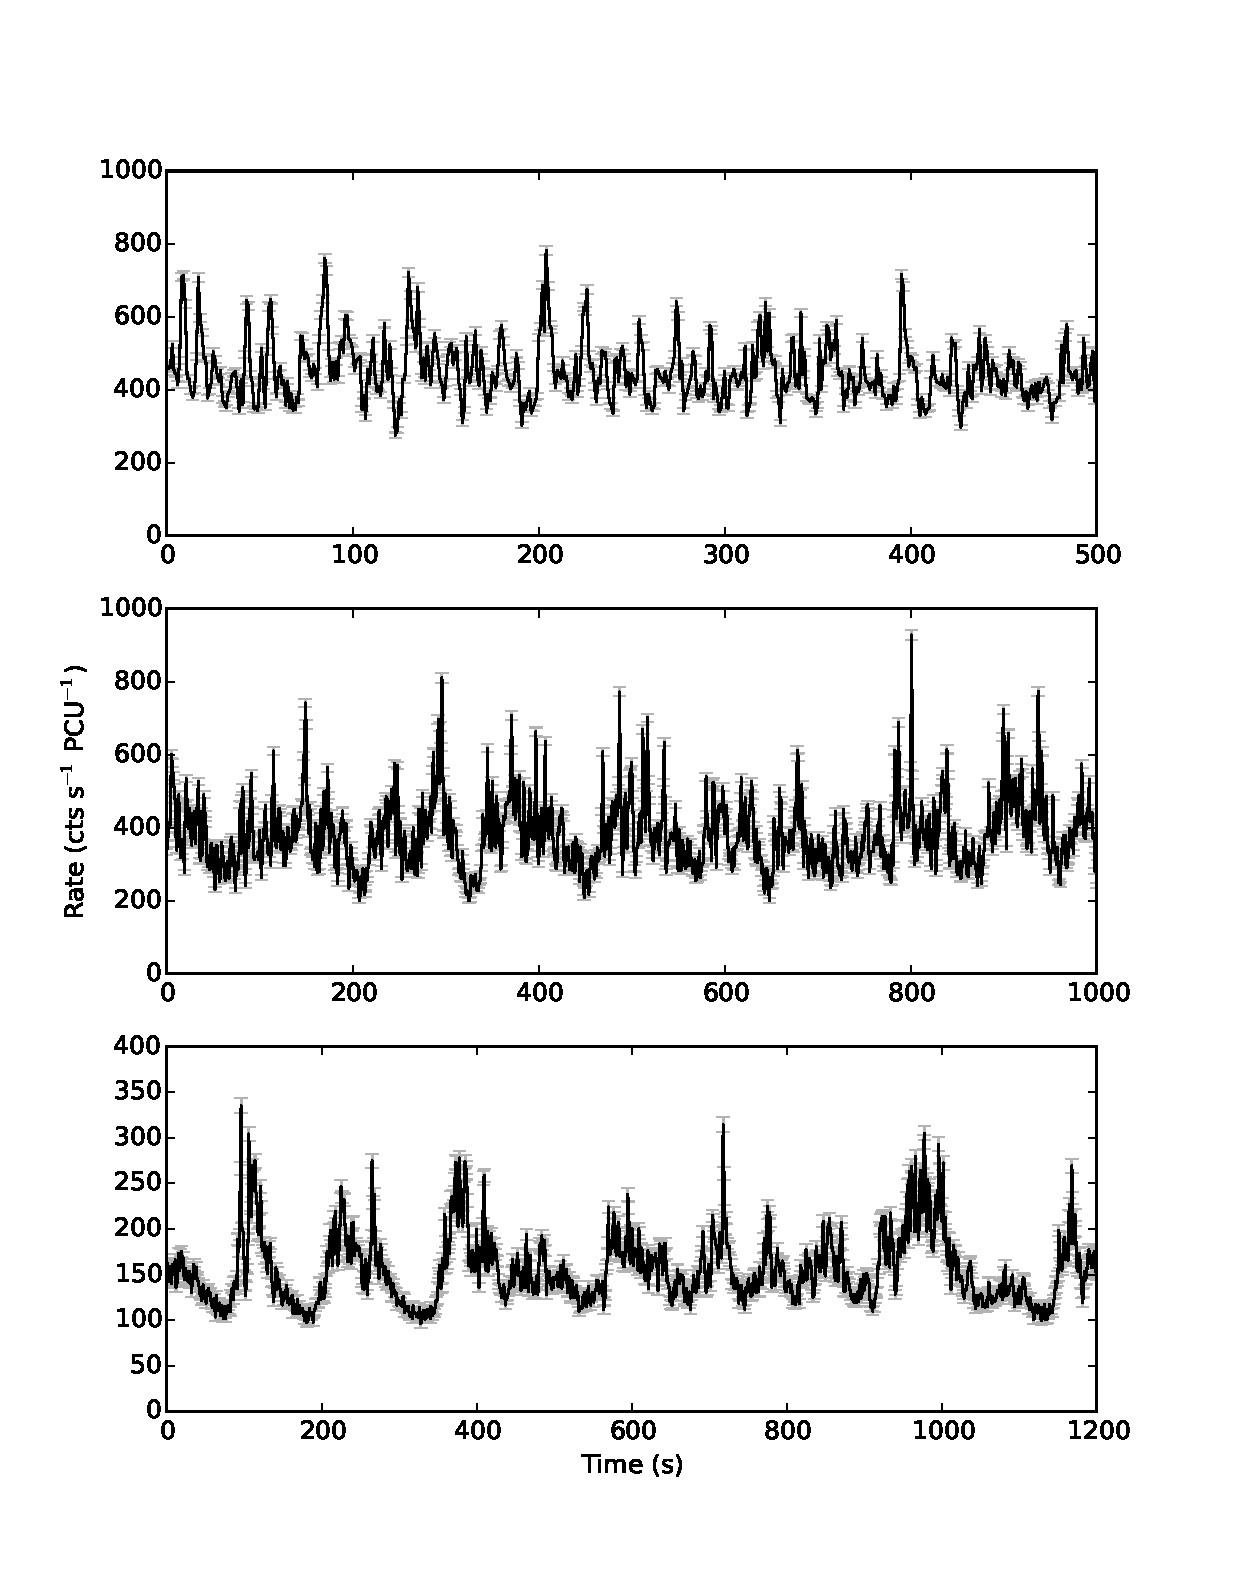
\includegraphics[width=.9\linewidth, trim={0.8cm 0 1.5cm 0},clip]{images/many_struc.eps}
  \caption[A selection of \textit{RXTE} lightcurves from Structured Bursting observations of the Bursting Pulsar.]{\small A selection of \indexrxte\textit{RXTE} lightcurves\index{Lightcurve} from Structured Bursting\index{Structured bursting} observations of the Bursting Pulsar\index{Bursting Pulsar}.  \textbf{Top:} a lightcurve from Outburst\index{Outburst} 1 showing flaring\index{Flare} on timescales of $\sim10$\,s.  \textbf{Middle:} a lightcurve from Outburst 1 showing the same flaring behaviour with an additional slower modulation over $\sim50$\,s.  \textbf{Bottom:} a lightcurve from Outburst 2 showing a regular sequence of flat-bottomed dips\index{Dip} and multi-peaked flaring.  These show the wide variety of variability\index{Variability} patterns that I classify as `Structured Bursting'.}
  \label{fig:Types_Struc}
\end{figure}

\section{Discussion}

\par I analyse all available X-ray data from the first 3 outbursts\index{Outburst} of the Bursting Pulsar\index{Bursting Pulsar}.  The bursting\index{X-ray burst} behaviour evolves in a similar way during these outbursts, strongly associating them with the Bursting Pulsar and suggesting an underlying connection between the classes of burst.  I also find that both Outbursts 1 \& 2 showed `rebrightening events'\index{Re-flare} similar to those seen in a number of other LMXBs\index{X-ray binary!Low mass} (e.g. \citealp{Wijnands_1808,Patruno_Reflares2}), including IGR J17091\index{IGR J17091-3624}.
\par I find that the X-ray\index{X-ray burst} bursts from these data can be best described as belonging to four phenomenological classes: Normal Bursts\index{Normal burst}, Minibursts\index{Miniburst}, Mesobursts\index{Mesoburst} and Structured Bursts\index{Structured bursting}.  For each of these four classes, I collect a number of statistics to shed light on the physical mechanisms that generate these lightcurve\index{Lightcurve} features.
\par Normal Bursts\index{Normal burst} and Minibursts\index{Miniburst} both represent the `Type II'\index{X-ray burst!Type II} bursting behaviour which is observed most commonly from this source.   Mesobursts\index{Mesoburst} occur much later on in the outburst and show fast-rise slow-decay profiles; they are generally much fainter and more structured than Normal Bursts.  Finally, Structured Bursts\index{Structured bursting} form continuous highly structured regions of variability\index{Variability} over timescales of days.  All Normal Bursts and some Minibursts show count rate `dips'\index{Dip} after the main burst, while Mesobursts and Structured Bursts do not.  In addition to this, some Normal and Mesobursts show count rate `plateaus'\index{Plateau}; regions of roughly stable count rate above the persistent level\index{Persistent emission} which last for $\sim10$s of seconds.  These features are also sometimes seen in Mesobursts, while Minibursts and Structured Bursts never show these structures.
\par Here I discuss these results in the context of models proposed to explain Type II\index{X-ray burst!Type II} bursting.  I also compare my results with those of previous studies on bursting in both the Bursting Pulsar\index{Bursting Pulsar} and the Rapid Burster\index{Rapid Burster}.

\subsection{Evolution of Outburst and Bursting Behaviour}

\par In general, Outburst\index{Outburst} 1 was brighter than Outburst\index{Outburst} 2, with the former having a peak 2--60\,keV intensity a factor of $\sim1.7$ greater than the latter.  However, in Figure \ref{fig:global_ob} I show that both outbursts evolve in a similar way.  In both outbursts, the intensity of the Bursting Pulsar reaches a peak of order $\sim1$\,Crab before decreasing over the next $\sim100$ days to a level of a few tens of mCrab.  A few 10s of days after reaching this level, the lightcurves\index{Lightcurve} of both outbursts show a pronounced `rebrightening'\index{Re-flare} event, during which the intensity increases to $\sim100$\,mCrab for $\sim10$ days.  Outburst 1 shows a second rebrightening event $\sim50$ days after the first.  It is unclear whether any rebrightening events occurred in Outburst 3 due to a lack of late-time observations with soft X-ray telescopes.  X-ray `rebrightening' events have been seen after the outbursts of a number of other LMXBs\index{X-ray binary!Low mass} with both neutron star\index{Neutron star} and black hole\index{Black hole} primaries: including SAX J1808.4-3658\index{SAX J1808.4-3658} \citep{Wijnands_1808}, XTE J1650-500\index{XTE J1650-500} \citep{Tomsick_MiniOutbursts} and IGR J17091-3624\index{IGR J17091-3624} (see Section \ref{sec:igrobevo}).
\par As I have shown in Figures \ref{fig:ob_evo1} \& \ref{fig:ob_evo2}, the nature of bursts\index{X-ray burst} from the Bursting Pulsar\index{Bursting Pulsar} evolves in a similar way in both Outbursts\index{Outburst} 1 \& 2.  Starting from around the peak of each outburst, both Normal\index{Normal burst} and Minibursts\index{Miniburst} are observed.  The fluence of these bursts decrease over time as the X-ray intensity of the source decreases, before bursting shuts off entirely when the 2--16\,keV flux falls below $\sim0.1$\,Crab.  After a few 10s of days with no bursts, bursting switches back on in the form of Mesobursts\index{Mesoburst}; this occurs during the tail of a rebrightening\index{Re-flare} event in Outburst 1, but in the tail of the main outburst in Outburst 2.  Mesobursting continues until the 2--16\,keV source flux falls below $\sim0.03$\,Crab, at which point I observe the onset of Structured Bursting\index{Structured bursting}.  In both Outbursts, Structured Bursting stops being visible a few 10s of days later during the start of a rebrightening event.  Because this evolution is common to both of the outbursts observed by \indexrxte\textit{RXTE}, this strongly indicates that the nature of bursting in the Bursting Pulsar\index{Bursting Pulsar} is connected with the evolution of its outbursts.  Additionally, with the exceptions of Normal and Minibursts, I show that each class of burst is mostly found in a distinct part of the outburst corresponding to a different level of persistent emission\index{Persistent emission}.
\par In Figure \ref{fig:meso_to_struc}, I show lightcurves\index{Lightcurve} from Outburst\index{Outburst} 2 taken a few days before and after the transition from Mesobursts\index{Mesoburst} to Structured Bursting\index{Structured bursting}.  We can see that, as the system approaches this transition, Mesobursts become more frequent and decrease in amplitude.  Additionally in Figure \ref{fig:meso_in_struc} I show a lightcurve which contains both a Mesoburst and Structured Bursting.  I find that, instead of a well-defined transition between these bursting classes, there is a more gradual change as Mesobursting evolves into Structured Bursting.
\par The transition between Normal Bursts\index{Normal burst} and Mesobursts\index{Mesoburst}, however, is not smooth; in both outbursts\index{Outburst} these two classes of bursting\index{X-ray burst} are separated by $\sim10$ day gaps in which no bursts of any kind were observed at all.  If all my classes of burst are caused by the same or similar processes, any model to explain them will also have to explain these periods with no bursts.

\begin{figure}
  \centering
  \includegraphics[width=.9\linewidth, trim={3.7cm 0cm 4.2cm 0cm},clip]{images/meso_evo.eps}
  \caption[A series of lightcurves from \textit{RXTE}/PCA observations of Outburst 2, showing a gradual evolution from Mesobursts to Structured Bursting over a period of $\sim30$ days.]{\small A series of lightcurves\index{Lightcurve} from \indexpca\textit{RXTE}/PCA observations of Outburst\index{Outburst} 2, showing a gradual evolution from Mesobursts\index{Mesoburst} to Structured Bursting\index{Structured bursting} over a period of $\sim30$ days.  Each inset lightcurve is plotted with the same $y$-scaling, and each corresponds to 2\,ks of data.}
  \label{fig:meso_to_struc}
\end{figure}

\subsection{Parameter Correlations}

\par I extracted a number of phenomenological parameters from each Normal Burst\index{Normal burst}, Miniburst\index{Miniburst} and Mesoburst\index{Mesoburst}.  For Normal Bursts, I extracted a large number of parameters by fitting a phenomenological model described in Section \ref{sec:struc}.  For Minibursts and Mesobursts I extracted recurrence times\index{Recurrence time} and persistent emission\index{Persistent emission}-subtracted peak rates; I also calculated burst\index{X-ray burst} fluences by integrating the persistent emission\index{Persistent emission}-subtracted rate over the duration of the burst.  I do not extract similar parameters for Structured Bursts\index{Structured bursting} due to their complex nature.
\par  In all three of the classes of burst\index{X-ray burst} I consider, I found that fluence and peak rate correlate strongly with persistent emission\index{Persistent emission}.  For each type of burst, the slope of these correlations is consistent with being equal during Outbursts\index{Outburst} 1 \& 2.
\par I also compared the Normal Bursts\index{Normal burst} in Outburst\index{Outburst} 1 with the Normal Bursts in Outburst 2.  The only significant statistical differences I found between these two populations\index{Population study} were in the burst peak rate and the burst fluence; both of these parameters are generally higher for Normal Bursts in Outburst 1.  As both of these parameters strongly depend on the persistent emission\index{Persistent emission}, both of these differences can be attributed to the fact that Outburst 1 was significantly brighter at peak than Outburst 2.
\par For Normal Bursts\index{Normal burst}, I found additional correlations.  Of particular note, I found that both the fall time and the recovery timescale of a `dip'\index{Dip} is proportional to its amplitude, which has implications for the possible mechanism behind these features.  I discuss this further in Section \ref{sec:mod}.
\par My findings strongly suggest that the properties of Normal\index{Normal burst}, Mini\index{Miniburst} and Mesobursts\index{Mesoburst} all depend on the persistent luminosity\index{Persistent emission} of the Bursting Pulsar\index{Bursting Pulsar}.  Assuming that this persistent luminosity is proportional to $\dot{M}$\index{Accretion rate}\index{M dot@$\dot{M}$|see {Accretion rate}}, this suggests that all classes of bursting\index{X-ray burst} are sensitive to the accretion rate of the system.  Additionally, with the exceptions of Normal and Minibursts, I find that each class of burst is mostly found in a distinct part of the outburst \index{Outburst}corresponding to a different level of persistent emission\index{Outburst}.  I suggest that Normal, Meso and Structured Bursts may in fact be manifestations of the same physical disk\index{Accretion disk} instability\index{Instability} but at different accretion rates.  This is supported by the observation of a Mesoburst during a period of Structured Bursting, which I show in the lightcurve in Figure \ref{fig:meso_in_struc}.  This shows that the conditions for both Mesobursts and Structured Bursting can be met at the same time.

\subsection{Comparison with Previous Studies}

\par In their study of bursts\index{X-ray burst} in the Bursting Pulsar\index{Bursting Pulsar}, \citet{Giles_BP} found evidence for three distinct classes of Type II\index{X-ray burst!Type II} bursts in the Bursting Pulsar:

\begin{itemize}
\item `Bursts' (hereafter G$_1$ Bursts to avoid confusion), the common Type II\index{X-ray burst!Type II} bursts\index{X-ray burst} seen from the source.
\item `Minibursts' (hereafter G$_2$  Bursts), with smaller amplitudes up to $\sim2$ times the persistent emission\index{Persistent emission} level.
\item `Microbursts' (hereafter G$_3$  Bursts), second-scale bursts with amplitudes of $\sim50$--$100\%$ of the persistent level.
\end{itemize}

We find that \citeauthor{Giles_BP}'s G$_1$ category contains the bursts that I identify as Normal Bursts\index{Normal burst}, while my Miniburst\index{Miniburst} category contains the same bursts as \citeauthor{Giles_BP}'s G$_2$ category.  \citeauthor{Giles_BP} only consider bursts\index{X-ray burst} up to MJD 50204 in their classification, and they could not classify any bursts that I identify as Mesobursts\index{Mesoburst}; under their framework, I find that Mesobursts would also be categorised as G$_1$.  I present the full mapping between \citeauthor{Giles_BP}'s classes and my classes in a schematic way in Table \ref{tab:classcomp}.

\begin{table}
\centering
\begin{tabular}{c c}
\hline
\hline
 \scriptsize My Class & \scriptsize \citeauthor{Giles_BP} Class  \\
\hline
Normal Bursts\index{Normal burst} & G$_1$ \\
Mesobursts\index{Mesoburst} & G$_1$ \\
Minibursts\index{Miniburst} & G$_2$ \\
Structured Bursts\index{Structured bursting} & - \\
 - & G$_3$ \\
\hline
\hline
\end{tabular}
\caption[A table showing how my burst classes for the Bursting Pulsar map to those described in \citet{Giles_BP}.]{A table showing how my burst\index{X-ray burst} classes map to those described in \citet{Giles_BP}.  \citeauthor{Giles_BP} do not consider the times during the outburst\index{Outburst} when Structured Bursts appear, and I consider G$_3$ bursts described by \citeauthor{Giles_BP} to be consistent with flicker noise.}
\label{tab:classcomp}
\end{table}

\par \citet{Giles_BP} note the presence of both dips\index{Dip} and plateaus\index{Plateau} in Normal Bursts.  To calculate the fluence of each main burst\index{X-ray burst} and its associated dip, \citeauthor{Giles_BP} integrate the total persistent-emission\index{Persistent emission}-subtracted counts in each feature.  They calculate that ratio between burst fluence and `missing' dip fluence ($\phi_{B}/\phi_{d}$) is between 0.26 and 0.56 in Outburst 1\index{Outburst} before correcting for dead-time\index{Dead-time} effects.  Using bursts in which my mathematical fit gave well-constrained ($>5\,\sigma$) values for both burst and dip fluence, I find that $\phi_{B}/\phi_{d}$ is between 1.3 and 2.0 in Outburst 1 and between 1.3 and 2.9 in Outburst 2.  My values differ significantly from those reported from \citeauthor{Giles_BP}; this is likely due to differing definitions of the persistent emission level\index{Persistent emission} and the start and end times of each dip, as \citeauthor{Giles_BP} do not report how they define these features.
\par My values for the ratios between burst\index{X-ray burst} and dip\index{Dip} fluences, as well as those of \citeauthor{Giles_BP}, are affected by dead-time\index{Dead-time}.  These effects cause the fluence of bursts to be under-reported, as can be inferred from Figure \ref{fig:minidips}, but the integrated counts in dips are not significantly affected \citep{Giles_BP}.  Therefore correcting for dead-time can only increase the value of $\phi_{B}/\phi_{d}$, and my result shows that the fluence of a burst is always greater than the fluence `missing' from a dip.
\par \textsf{T.O.} and I find evidence of significant colour\index{Colour}\index{Hysteresis} evolution during both Normal Bursts\index{Normal burst} and Minibursts\index{Miniburst}, which is strongly indicative of a spectral\index{Spectroscopy} evolution (see also e.g. \citealp{Woods_OB2}).  Further work on the time-resolved spectra of this source will likely allow us to better understand the underlying physics of its behaviour.
\par Using data from the KONUS\index{KONUS} experiments aboard the \textit{GGS-Wind}\index{GGS-Wind@\textit{GGS-Wind}} and \textit{Kosmos-2326}\index{Kosmos-2326@\textit{Kosmos 2326}} satellites, \citet{Aptekar_Recur} have previously found that the recurrence times\index{Recurrence time} between consecutive bursts\index{X-ray burst} in Outburst\index{Outburst} 1 are distributed with a constant mean of $\sim1776$\,s.  This is substantially longer than the value of 1209\,s that I find for Outburst 1, but my value is likely an underestimate due to a selection bias caused by the relatively short pointings of \indexrxte\textit{RXTE}.
\par Using \indexchandra\textit{Chandra} and \indexxmm\textit{XMM-Newton} data, I find a mean recurrence time\index{Recurrence time} for Outburst\index{Outburst} 3 of 1986\,s; as pointings with these instruments are significantly longer than the burst recurrence timescale, windowing effects are negligible.  As this value is close to the value that \citet{Aptekar_Recur} find for mean recurrence time, my result is consistent with the burst\index{X-ray burst} rate in all three outbursts being approximately the same.
\par Previous studies with \index{CGRO@\textit{CGRO}!BATSE}\index{CGRO@\textit{CGRO}}\textit{CGRO}/BATSE have found that the burst\index{X-ray burst} rate during the first few days of Outbursts\index{Outburst} 1 \& 2 was significantly higher than during the rest of each outburst \citep{Kouveliotou_BP,Woods_OB2}.  As \indexrxte\textit{RXTE} did not observe either of these times, I am unable to test this result with my dataset.

\subsection{Comparison with other objects}

\par Another natural comparison to the Bursting Pulsar\index{Bursting Pulsar} is the Rapid Burster\index{Rapid Burster} \citep{Lewin_RBDiscovery}, a neutron star\index{Neutron star} LMXB\index{X-ray binary!Low mass} in the globular cluster Liller I\index{Liller 1}.  This object is the only LMXB other than the Bursting Pulsar known to unambiguously exhibit Type II\index{X-ray burst!Type II} bursting behaviour during outbursts\index{Outburst}.  \citet{Rappaport_BPHistory} have previously proposed that the Bursting Pulsar, the Rapid Burster and other neutron star LMXBs form a continuum of objects with different magnetic field\index{Magnetic field} strengths.
\par I compare my study of bursts\index{X-ray burst} in the Bursting Pulsar\index{Bursting Pulsar} with studies of Type II\index{X-ray burst!Type II} bursts in the Rapid Burster\index{Rapid Burster}, particularly the detailed population study\index{Population study} performed by \citet{Bagnoli_PopStudy}.  \citet{Bagnoli_PopStudy} found that Type II bursting begins during the decay of an outburst\index{Outburst} in the Rapid Burster.  This is the same as what we see in the Bursting Pulsar, where I find Normal Bursting\index{Normal burst} behaviour starts during the outburst decay.  \citet{Bagnoli_PopStudy} found that all bursting in the Rapid Burster shuts off above an Eddington Fraction\index{Eddington limit} of $\gtrsim0.05$, whereas I find that bursting in the Bursting Pulsar shuts off \textit{below} a 2--16\,keV flux of Eddington fraction of $\sim0.1$\,Crab: assuming that the peak persistent luminosity of the Bursting Pulsar was approximately Eddington Limited (e.g. \citealp{Sazonov_BPGranat}), this value corresponds to an Eddington fraction of order $\sim0.1$.  This suggests that Type II bursting in these two objects happen in very different accretion rate\index{Accretion rate} regimes.
\par \citet{Bagnoli_PopStudy} showed that bursting\index{X-ray burst!Type II} behaviour in the Rapid Burster\index{Rapid Burster} falls into a number of `bursting modes', defined by the morphology of individual Type II bursts.  In particular, they find that Type II bursts in the Rapid Burster fall into two classes (see also \citealp{Marshall_2types}), lightcurves\index{Lightcurve} of which I reproduce in Figure \ref{fig:bagnoli_lcs}:

\begin{figure}
  \centering
  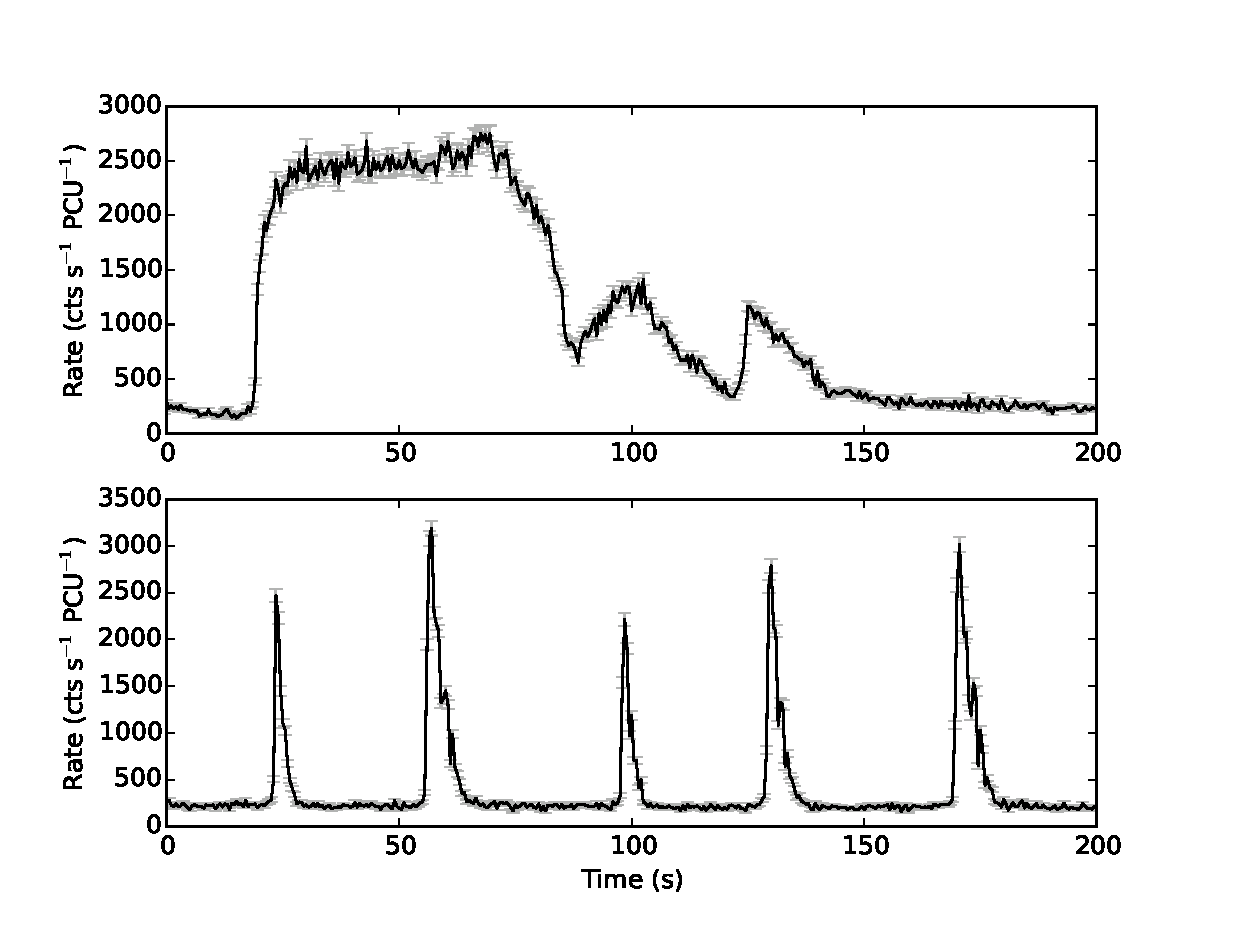
\includegraphics[width=.9\linewidth, trim={0.8cm 0 1.4cm 0},clip]{images/bagnoli_bursts.eps}
  \caption[\textit{RXTE} lightcurves of representative Long (top) and Short (bottom) Type II bursts from the Rapid Burster.]{\small \indexrxte\textit{RXTE} lightcurves\index{Lightcurve} of representative Long (top) and Short (bottom) Type II bursts\index{X-ray burst!Type II} from the Rapid Burster\index{Rapid Burster}.  These bursts were identified and classified by \citet{Bagnoli_PopStudy}.}
  \label{fig:bagnoli_lcs}
\end{figure}

\begin{itemize}
\item Short near-symmetric Bursts\index{X-ray burst!Type II} with timescales of $\sim10$s of seconds and peak rates near the Eddington Limit\index{Eddington limit}.
\item Long bursts with a fast rise, a long $\sim100$\,s plateau\index{Plateau} at peak rate followed by a fast decay.  The level of the plateau is generally at or near the Eddington Limit.
\end{itemize}

\par Short bursts\index{X-ray burst!Type II} are very similar in shape to Normal Bursts\index{Normal burst} in the Bursting Pulsar\index{Bursting Pulsar}, but I find no analogue of long bursts in my study.  \citet{Bagnoli_PopStudy} suggests that the `flat-top' profile of long bursts could be due to the effects of near-Eddington\index{Eddington limit} accretion\index{Accretion}, and they show that the intensity at the top of these bursts is close to Eddington limit.  Previous works have shown that the persistent emission\index{Persistent emission} of the Bursting Pulsar is Eddington-limited at peak, and therefore bursts\index{X-ray burst} from the Bursting Pulsar are significantly super-Eddington\index{Super-Eddington accretion} \citep{Sazonov_BPGranat}.   I suggest, therefore, that Long Bursts cannot occur in systems with a persistent rate approaching the Eddington Limit.  This could explain why Long Bursts are not seen during periods of Normal Bursting\index{Normal burst} in the Bursting Pulsar (during which the persistent emission is $\gtrsim{20}$\% of Eddington), but it remains unclear why these features are not seen later in each outburst\index{Outburst} when the Bursting Pulsar is fainter.  Alternatively, all the differences we see between bursts produced by the Rapid Burster\index{Rapid Burster} and the Bursting Pulsar could be explained if the physical mechanisms behind these bursts are indeed different between the objects.
\par \citet{Bagnoli_PopStudy} also find a number of correlations between burst\index{X-ray burst!Type II} parameters in the Rapid Burster\index{Rapid Burster}, which I can compare with my results for the Bursting Pulsar\index{Bursting Pulsar}.  I find a number of similarities between the two objects:

\begin{itemize}
\item The fluence of a burst correlates with its amplitude.
\item The duration of a burst does not correlate\footnote{We state two parameters do not correlate if their Spearman Rank score corresponds to a significance $<3\sigma$.} with the persistent emission\index{Persistent emission}.
\item The recurrence time\index{Recurrence time} between consecutive bursts does not depend on the persistent emission.
 \end{itemize}

\par There are also a number of differences between the set of correlations between burst\index{X-ray burst} parameters in these two systems:

\begin{itemize}
\item Burst duration is correlated with burst fluence in the Rapid Burster\index{Rapid Burster}, but these have not been seen to correlate in the Bursting Pulsar\index{Bursting Pulsar}.
\item Burst duration, peak rate and burst fluence are all correlated with burst recurrence time\index{Recurrence time} in the Rapid Burster.  I have not found any of these parameters to correlate with burst recurrence time in the Bursting Pulsar.
\item Peak rate and burst fluence correlate with persistent emission\index{Persistent emission} in the Bursting Pulsar, but this is not true for bursts of a given type in the Rapid Burster.
\end{itemize}

\par As the neither the fluence nor the class of a burst in the Rapid Burster\index{Rapid Burster} depend strongly on persistent emission\index{Persistent emission}, and hence $\dot{M}$\index{Accretion rate}, this suggests that the process that triggers Type-II\index{X-ray burst!Type II} bursts in this source is not strongly dependent on the global accretion rate.  However the strong correlations between persistent emission and burst peak and fluence I find in the Bursting Pulsar\index{Bursting Pulsar} show that the energetics of individual bursts\index{X-ray burst} strongly depend global accretion rate at that time.
\par It has previously been noted that consecutive Normal Bursts\index{Normal burst} in the Bursting Pulsar\index{Bursting Pulsar} do not show a strong correlation between recurrence time\index{Recurrence time} and fluence (\citealp{Taam_Evo,Lewin_BP}, however see \citealp{Aptekar_OscRel}).  This correlation would be expected if the instability\index{Instability} took the form of a relaxation oscillator\index{Relaxation oscillator}, as it does in the Rapid Burster\index{Rapid Burster} \citep{Lewin_TypeII}.  However, I also find that the arrival times of Normal Bursts from the Bursting Pulsar are not consistent with a Poisson distribution\index{Poisson distribution} with constant mean.  This implies either that bursts are also not independent events in the Bursting Pulsar, or that the frequency of these bursts is not constant throughout an outburst as reported by \citet{Aptekar_Recur}.
\par In Chapter \ref{ch:BPletter} I discuss the possibility that some of the behaviour in the Bursting Pulsar\index{Bursting Pulsar} could be due to fluctuations in the magnetospheric radius\index{Magnetospheric radius} of the system close to the co-rotation\index{Co-rotation radius} radius.  This behaviour, referred to in this thesis as `hiccup' accretion\index{Hiccup accretion}, (e.g. \citealp{Bogdanov_TMSPVar,Ferrigno_TMSPVar}) is also seen in `Transitional Millisecond Pulsars'\index{TMSP}\index{Transitional millisecond pulsar|see {TMSP}} (TMSPs): objects which alternate between appearing as X-ray pulsars\index{Pulsar} and radio pulsars (see e.g. \citealp{Archibald_Link,Papitto_Swings}).

\subsection{Comparison with Models of Type II Bursts}

\label{sec:mod}

\par All of the models of Type II\index{X-ray burst!Type II} bursting which we discuss in Section \ref{sec:TIImod} are able to reproduce some of the features we see from bursts\index{X-ray burst} in the Bursting Pulsar\index{Bursting Pulsar}.  In particular, the `dip'\index{Dip} we see after Normal Bursts\index{Normal burst} has previously been interpreted as being caused by the inner disk\index{Accretion disk}\index{Disk|see {Accretion disk}} refilling after a sudden accretion\index{Accretion} event (e.g. \citealp{Younes_Expo}).  \label{sec:Mini_Norm}As these dips are also seen after some Minibursts\index{Miniburst}, we could also interpret Minibursts as being caused by a similar cycle.  To test this idea, in Figure \ref{fig:minidips} I present a scatter plot of the burst and dip fluences for all Normal Bursts and Minibursts.  In both classes of burst, there is a strong correlation between these two parameters.  I find that a power law fit to the Normal Bursts in this parameter space also describes the Minibursts.  This suggests that the same relationship between burst fluence and missing dip fluence holds for both types of burst, although the two populations\index{Population study} are not continuous.  This suggests that Minibursts are energetically consistent with being significantly fainter versions of Normal Bursts.

\begin{figure}
  \centering
  \includegraphics[width=.9\linewidth, trim={0cm 0 0cm 0},clip]{images/minidips.eps}
  \caption[A scatter plot showing the relationship between burst fluence and `missing' dip fluence for Normal Bursts and Minibursts.]{\small A scatter plot showing the relationship between burst\index{X-ray burst} fluence and `missing' dip\index{Dip} fluence for Normal Bursts\index{Normal burst} (black) and Minibursts\index{Miniburst} (Red), with the best fit power law plotted in solid blue.  A power law fit to just the Normal Bursts (blue dashed line) also approaches the Minibursts.  Note that the Normal Bursts plotted in grey were not used to calculate this latter fit, as the effects of instrumental dead-time\index{Dead-time} cause high burst fluences to be under-reported.  Upper limits on Miniburst dip fluences are shown with arrows.}
  \label{fig:minidips}
\end{figure}

\par The models of \citet{Spruit_Type2Mod} and \citet{Walker_Type2Mod} have shortcomings when used to describe the Bursting Pulsar\index{Bursting Pulsar}.  \citet{Walker_Type2Mod} state that their model only produces Type II\index{X-ray burst!Type II} bursts for a very specific set of criteria on the system parameters.   One of these criteria is an essentially non-magnetic\index{Magnetic field} ($B=0$) neutron star\index{Neutron star}.  This is inconsistent with observations of cyclotron lines\index{Cyclotron lines} from the Bursting Pulsar and the presence of a persistent pulsar\index{Pulsar}, both of which suggest a surface field strength of order 10$^{11}$\,G \citep{Doroshenko_NBFlash}.
\par Unlike models based on viscous\index{Viscosity} instability\index{Instability}, the model of \citet{Spruit_Type2Mod} does not impose a correlation between burst\index{X-ray burst} fluence and burst recurrence time\index{Recurrence time} (see e.g. the evaluation of this model in the context of the Rapid Burster\index{Rapid Burster} performed by \citealp{Bagnoli_PopStudy}).  However, it does predict a strong correlation between burst recurrence time and mean accretion rate\index{Accretion rate}, which is not consistent with my results for the Bursting Pulsar\index{Bursting Pulsar}.
\par In general, I find that models established to explain bursting\index{X-ray burst} in the Rapid Burster\index{Rapid Burster} are poor at explaining bursting in the Bursting Pulsar\index{Bursting Pulsar}.  Any model which can produce Type II\index{X-ray burst!Type II} bursting in both systems fails to explain why other systems do not also show this behaviour.  My results suggest that Type II bursts in the Rapid Burster and the Bursting Pulsar may require two separate models to be explained.

\subsubsection{Evidence of Thermonuclear Burning}

\label{sec:nuc}

\par I also consider the possibility that some of my observations could be explained by thermonuclear burning\index{Thermonuclear burning} on the Bursting Pulsar\index{Bursting Pulsar}.  A thermonuclear origin for the main part of Normal Bursts\index{Normal burst} has been ruled out by previous authors (e.g. \citealp{Lewin_BP}), but it is less clear that associated features could not be explained by this process.
\par It has been shown that, above a certain accretion rate\index{Accretion rate}, thermonuclear burning\index{Thermonuclear burning} on the surface of a neutron star\index{Neutron star} should be stable; below this rate, thermonuclear burning takes place in the form of Type I\index{X-ray burst!Type I} bursts (e.g. \citealp{Fujimoto_Shellstab,Bildsten_Regimes}).  \citet{Bildsten_Nuclear} have previously studied which form thermonuclear burning on the Bursting Pulsar\index{Bursting Pulsar} would take.  They find that the presence and profile of a thermonuclear burning event on the Bursting Pulsar would be strongly dependent on both the accretion rate $\dot{M}$ and the magnetic field\index{Magnetic field} strength $B$.  They predict that, for $B\gtrsim3\times10^{10}$\,G, burning events would take the form of a slowly propagating burning front which would result in a low-amplitude X-ray burst\index{X-ray burst} with a timescale of several minutes.  Measurements of the Bursting Pulsar taken during Outburst\index{Outburst} 3 suggest a surface field strength of $>10^{11}$\,G, in turn suggesting that the Bursting Pulsar exists in the regime in which this burning behaviour is possible.
\par The `plateau'\index{Plateau} events after Normal Bursts\index{Normal burst} are consistent with the slow burning\index{Thermonuclear burning} predicted by \citet{Bildsten_Nuclear}.  This picture is consistent with models for Type II\index{X-ray burst!Type II} X-ray bursts involving spasmodic accretion\index{Accretion} events (e.g. \citealp{Spruit_Type2Mod,Walker_Type2Mod}), as plateaus\index{Plateau} always occur after a Type II-like burst\index{X-ray burst} has deposited a large amount of ignitable material onto the neutron star\index{Neutron star} surface.  However in this picture it would be unclear why many Normal Bursts\index{Normal burst} do not show this plateau feature.  Mesobursts\index{Mesoburst} can also exhibit plateaus, and are therefore may also be products of spasmodic accretion onto the neutron star.
\par However, the interpretation of Mesobursts\index{Mesoburst} as being caused by discrete accretion\index{Accretion} events is difficult to reconcile with the fact that these features never show dips\index{Dip}.  \citet{Bildsten_Nuclear} show that, at smaller values of $\dot{M}$\index{Accretion rate}, nuclear burning\index{Thermonuclear burning} on the Bursting Pulsar\index{Bursting Pulsar} could become unstable.  Mesobursts are only seen during the latter stages of Outbursts\index{Outburst} 1 \& 2, when the accretion rate is well below 0.1 Eddington\index{Eddington limit}.  An interesting alternative possibility is that Mesobursts are a hybrid event, consisting of a flash of unstable thermonuclear X-ray burning followed by a slower quasi-stable burning of residual material in the form of a propagating burning front.
\par This picture would also be able to explain why Mesobursts\index{Mesoburst} are only seen during the latter parts of each outburst\index{Outburst}.  As the accretion rate\index{Accretion rate} onto the Bursting Pulsar\index{Bursting Pulsar} approaches Eddington\index{Eddington limit} during the peak of its outbursts, it is likely that the accretion rate is high enough that only stable burning\index{Thermonuclear burning} is permitted.  During the smaller rebrightening\index{Re-flare} events after the main part of each outburst, the accretion rate is $\sim1$--2 orders of magnitude lower, and hence the system may then be back in the regime in which Type I\index{X-ray burst!Type I} burning is possible.  Additional studies of the spectral\index{Spectroscopy} evolution of Mesobursts will be required to further explore this possibility.
\par Previous authors have discussed the possibility of a marginally stable burning\index{Thermonuclear burning} regime on the surface of neutron stars\index{Neutron star} (not to be confused with the previously mentioned quasi-stable burning).  In this regime, which occurs close to the boundary between stable and unstable burning, \citet{Heger_MargStab} showed that an oscillatory mode of burning may occur.  They associated this mode of burning with the mHz QPOs\index{Quasi-periodic oscillation} which have been observed in a number of neutron star LMXBs\index{X-ray binary!Low mass} (e.g. \citealp{Revnivtsev_MargStab,Altamirano_MargStab}).  These QPOs only occur over a narrow range of source luminosities, show a strong decrease in amplitude at higher energies, and they disappear after a Type I\index{X-ray burst!Type I} burst (e.g. \citealp{Altamirano_MargStab}).
\par Lightcurves\index{Lightcurve} of objects undergoing marginally stable burning\index{Thermonuclear burning} qualitatively resemble those of Structured Bursting\index{Structured bursting} in the Bursting Pulsar\index{Bursting Pulsar}, raising the possibility of a thermonuclear explanation for Structured Bursting.  However, as I show in Figure \ref{fig:ob_evo1}, Structured Bursting during Outburst\index{Outburst} 1 occurred during a period of time in which the Bursting Pulsar's luminosity changed by $\sim1$ order of magnitude.  In addition to this, in Figure \ref{fig:meso_in_struc} I show an example of a Mesoburst\index{Mesoburst} during a period of Structured Bursting.  If Mesobursts can be associated with Type I\index{X-ray burst!Type I} bursts, any marginally stable burning on the surface of the Bursting Pulsar should have stopped after this event.  Due to these inconsistencies with observations of marginally stable burning on other sources, it is unlikely that Structured Bursting is a manifestation of marginally stable burning on the Bursting Pulsar.
\par \citet{Linares_MargStab} observed yet another mode of thermonuclear burning\index{Thermonuclear burning} during the 2010 outburst of the LMXB\index{X-ray binary!Low mass} Terzan 5 X-2\index{Terzan 5 X-2}.  They observed a smooth evolution from discrete Type I\index{X-ray burst!Type I} bursts into a period of quasi-periodic oscillations\index{Quasi-periodic oscillation} resembling Structured Bursting\index{Structured bursting}.  This behaviour resembles the evolution I observe between Mesobursts\index{Mesoburst} and Structured Bursting in Outbursts\index{Outburst} 1 \& 2 of the Bursting Pulsar\index{Bursting Pulsar} (as shown in Figure \ref{fig:meso_to_struc}; compare with Figure 1 in \citealp{Linares_MargStab}).  However there are a number of differences between the evolutions seen in both objects.  In Terzan 5 X-2 the recurrence timescale\index{Recurrence time} of Type I bursts during the evolution is strongly related to the accretion rate\index{Accretion rate} of the source at the time, whereas there is no such strong relation between the two in Mesobursts from the Bursting Pulsar.  Additionally, the quasi-periodic oscillations in Terzan 5 X-2 evolved smoothly back into Type I bursts later in the outburst, whereas Structured Bursting does not evolve back into Mesobursts in the Bursting Pulsar.  As such, it is unclear that Mesobursts and Structured Bursting can be associated with the unusual burning mode seen on Terzan 5 X-2.

\section{Conclusions}

\par I analyse all X-ray bursts\index{X-ray burst} from the Bursting Pulsar\index{Bursting Pulsar} seen by \indexpca\textit{RXTE}/PCA during its first and second outbursts\index{Outburst}, as well as bursts seen by other missions during the third outburst of the source.  I conclude that these bursts are best described as belonging to four separate classes of burst: Normal Bursts\index{Normal burst}, Mesobursts\index{Mesoburst}, Minibursts\index{Miniburst} and Structured Bursts\index{Structured bursting}.  I find that the bursting behaviour in these four classes evolves in a similar way throughout the first two outbursts of the Bursting Pulsar.  I present a new semi-mathematical model to fit to the Normal Bursts in this object.  Using this new framework, I will be able better quantify Bursting-Pulsar-like X-ray bursts when they are observed in other objects in the future.
\par I find the bursts\index{X-ray burst} in the Rapid Burster\index{Rapid Burster} and the Bursting Pulsar\index{Bursting Pulsar} to be different in burst profile, peak Eddington\index{Eddington limit} ratio, and durations.  While the fluence of bursts in the Bursting Pulsar depend strongly on the persistent emission\index{Persistent emission} at the time, this is not the case in the Rapid Burster.  Additionally the waiting time\index{Recurrence time} between bursts in the Rapid Burster depends heavily on the fluence of the preceding burst, but I do not find this in the Bursting Pulsar.  Therefore, it would be reasonable to conclude that the bursting in these two objects is generated by two different mechanisms.
\par However, it is also important to note a number of similarities between the Bursting Pulsar\index{Bursting Pulsar} and the Rapid Burster\index{Rapid Burster}.  Bursting behaviour in both objects depends on the global accretion rate\index{Accretion rate} of the system and the evolution of its outbursts\index{Outburst}.  Additionally, the recurrence times\index{Recurrence time} of bursts do not depend on persistent emission\index{Persistent emission} in either object, and nor does the duration of an individual burst\index{X-ray burst}.  Notably while Type II\index{X-ray burst!Type II} bursts in the Rapid Burster only occur at luminosities $L\lesssim0.05L_{Edd}$\index{Eddington limit}, I find that Normal bursts\index{Normal burst} in the Bursting Pulsar only occur at $L\gtrsim0.1L_{Edd}$.  There is no overlap between the luminosity regimes, in terms of the Eddington Luminosity, at which bursting is observed in the two objects.  This leads to the alternative hypothesis that bursts in the two systems may be caused by similar processes, but that these processes take place in very different physical regimes.